% Options for packages loaded elsewhere
\PassOptionsToPackage{unicode}{hyperref}
\PassOptionsToPackage{hyphens}{url}
%
\documentclass[
]{book}
\usepackage{amsmath,amssymb}
\usepackage{iftex}
\ifPDFTeX
  \usepackage[T1]{fontenc}
  \usepackage[utf8]{inputenc}
  \usepackage{textcomp} % provide euro and other symbols
\else % if luatex or xetex
  \usepackage{unicode-math} % this also loads fontspec
  \defaultfontfeatures{Scale=MatchLowercase}
  \defaultfontfeatures[\rmfamily]{Ligatures=TeX,Scale=1}
\fi
\usepackage{lmodern}
\ifPDFTeX\else
  % xetex/luatex font selection
\fi
% Use upquote if available, for straight quotes in verbatim environments
\IfFileExists{upquote.sty}{\usepackage{upquote}}{}
\IfFileExists{microtype.sty}{% use microtype if available
  \usepackage[]{microtype}
  \UseMicrotypeSet[protrusion]{basicmath} % disable protrusion for tt fonts
}{}
\makeatletter
\@ifundefined{KOMAClassName}{% if non-KOMA class
  \IfFileExists{parskip.sty}{%
    \usepackage{parskip}
  }{% else
    \setlength{\parindent}{0pt}
    \setlength{\parskip}{6pt plus 2pt minus 1pt}}
}{% if KOMA class
  \KOMAoptions{parskip=half}}
\makeatother
\usepackage{xcolor}
\usepackage{color}
\usepackage{fancyvrb}
\newcommand{\VerbBar}{|}
\newcommand{\VERB}{\Verb[commandchars=\\\{\}]}
\DefineVerbatimEnvironment{Highlighting}{Verbatim}{commandchars=\\\{\}}
% Add ',fontsize=\small' for more characters per line
\usepackage{framed}
\definecolor{shadecolor}{RGB}{248,248,248}
\newenvironment{Shaded}{\begin{snugshade}}{\end{snugshade}}
\newcommand{\AlertTok}[1]{\textcolor[rgb]{0.94,0.16,0.16}{#1}}
\newcommand{\AnnotationTok}[1]{\textcolor[rgb]{0.56,0.35,0.01}{\textbf{\textit{#1}}}}
\newcommand{\AttributeTok}[1]{\textcolor[rgb]{0.13,0.29,0.53}{#1}}
\newcommand{\BaseNTok}[1]{\textcolor[rgb]{0.00,0.00,0.81}{#1}}
\newcommand{\BuiltInTok}[1]{#1}
\newcommand{\CharTok}[1]{\textcolor[rgb]{0.31,0.60,0.02}{#1}}
\newcommand{\CommentTok}[1]{\textcolor[rgb]{0.56,0.35,0.01}{\textit{#1}}}
\newcommand{\CommentVarTok}[1]{\textcolor[rgb]{0.56,0.35,0.01}{\textbf{\textit{#1}}}}
\newcommand{\ConstantTok}[1]{\textcolor[rgb]{0.56,0.35,0.01}{#1}}
\newcommand{\ControlFlowTok}[1]{\textcolor[rgb]{0.13,0.29,0.53}{\textbf{#1}}}
\newcommand{\DataTypeTok}[1]{\textcolor[rgb]{0.13,0.29,0.53}{#1}}
\newcommand{\DecValTok}[1]{\textcolor[rgb]{0.00,0.00,0.81}{#1}}
\newcommand{\DocumentationTok}[1]{\textcolor[rgb]{0.56,0.35,0.01}{\textbf{\textit{#1}}}}
\newcommand{\ErrorTok}[1]{\textcolor[rgb]{0.64,0.00,0.00}{\textbf{#1}}}
\newcommand{\ExtensionTok}[1]{#1}
\newcommand{\FloatTok}[1]{\textcolor[rgb]{0.00,0.00,0.81}{#1}}
\newcommand{\FunctionTok}[1]{\textcolor[rgb]{0.13,0.29,0.53}{\textbf{#1}}}
\newcommand{\ImportTok}[1]{#1}
\newcommand{\InformationTok}[1]{\textcolor[rgb]{0.56,0.35,0.01}{\textbf{\textit{#1}}}}
\newcommand{\KeywordTok}[1]{\textcolor[rgb]{0.13,0.29,0.53}{\textbf{#1}}}
\newcommand{\NormalTok}[1]{#1}
\newcommand{\OperatorTok}[1]{\textcolor[rgb]{0.81,0.36,0.00}{\textbf{#1}}}
\newcommand{\OtherTok}[1]{\textcolor[rgb]{0.56,0.35,0.01}{#1}}
\newcommand{\PreprocessorTok}[1]{\textcolor[rgb]{0.56,0.35,0.01}{\textit{#1}}}
\newcommand{\RegionMarkerTok}[1]{#1}
\newcommand{\SpecialCharTok}[1]{\textcolor[rgb]{0.81,0.36,0.00}{\textbf{#1}}}
\newcommand{\SpecialStringTok}[1]{\textcolor[rgb]{0.31,0.60,0.02}{#1}}
\newcommand{\StringTok}[1]{\textcolor[rgb]{0.31,0.60,0.02}{#1}}
\newcommand{\VariableTok}[1]{\textcolor[rgb]{0.00,0.00,0.00}{#1}}
\newcommand{\VerbatimStringTok}[1]{\textcolor[rgb]{0.31,0.60,0.02}{#1}}
\newcommand{\WarningTok}[1]{\textcolor[rgb]{0.56,0.35,0.01}{\textbf{\textit{#1}}}}
\usepackage{longtable,booktabs,array}
\usepackage{calc} % for calculating minipage widths
% Correct order of tables after \paragraph or \subparagraph
\usepackage{etoolbox}
\makeatletter
\patchcmd\longtable{\par}{\if@noskipsec\mbox{}\fi\par}{}{}
\makeatother
% Allow footnotes in longtable head/foot
\IfFileExists{footnotehyper.sty}{\usepackage{footnotehyper}}{\usepackage{footnote}}
\makesavenoteenv{longtable}
\usepackage{graphicx}
\makeatletter
\def\maxwidth{\ifdim\Gin@nat@width>\linewidth\linewidth\else\Gin@nat@width\fi}
\def\maxheight{\ifdim\Gin@nat@height>\textheight\textheight\else\Gin@nat@height\fi}
\makeatother
% Scale images if necessary, so that they will not overflow the page
% margins by default, and it is still possible to overwrite the defaults
% using explicit options in \includegraphics[width, height, ...]{}
\setkeys{Gin}{width=\maxwidth,height=\maxheight,keepaspectratio}
% Set default figure placement to htbp
\makeatletter
\def\fps@figure{htbp}
\makeatother
\usepackage{soul}
\setlength{\emergencystretch}{3em} % prevent overfull lines
\providecommand{\tightlist}{%
  \setlength{\itemsep}{0pt}\setlength{\parskip}{0pt}}
\setcounter{secnumdepth}{5}
\usepackage{booktabs}
\ifLuaTeX
  \usepackage{selnolig}  % disable illegal ligatures
\fi
\usepackage[]{natbib}
\bibliographystyle{apalike}
\IfFileExists{bookmark.sty}{\usepackage{bookmark}}{\usepackage{hyperref}}
\IfFileExists{xurl.sty}{\usepackage{xurl}}{} % add URL line breaks if available
\urlstyle{same}
\hypersetup{
  pdftitle={Data Science for Social Scientists: An applied course using IPUMS data},
  hidelinks,
  pdfcreator={LaTeX via pandoc}}

\title{Data Science for Social Scientists: An applied course using IPUMS data}
\author{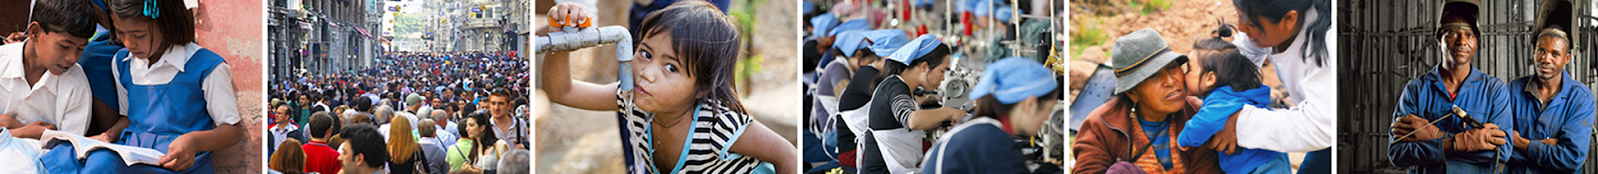
\includegraphics{ipums_banner.png}\\
\strut \\
\strut \\
\textbf{Developed by:}\\
\hspace*{0.333em}\hspace*{0.333em}\hspace*{0.333em}Daniel E. Ehrlich, \href{https://international.ipums.org/international/}{IPUMS, University of Minnesota}\\
\hspace*{0.333em}\hspace*{0.333em}\hspace*{0.333em}Anna Tremblay, \href{https://www.clemson.edu/cbshs/departments/sacj/degrees/anthropology.html}{Dept of Soc, Anth, \& CJ, Clemson University}\\
\hspace*{0.333em}\hspace*{0.333em}\hspace*{0.333em}Current Version compiled: 2024-02-26\\

\includegraphics[width=0.4\textwidth,height=\textheight]{ipums_i_logo.jpg} 
\includegraphics[width=0.4\textwidth,height=\textheight]{clemson_logo.png}\\
}
\date{}

\begin{document}
\maketitle

{
\setcounter{tocdepth}{1}
\tableofcontents
}
\hypertarget{preface}{%
\chapter*{Preface}\label{preface}}
\addcontentsline{toc}{chapter}{Preface}

An applied methods class for social scientists that uses real-world IPUMS data. This course is:

Open-source and customizable -\\
\hspace*{0.333em}\hspace*{0.333em}\hspace*{0.333em}All materials available on \href{https://github.com/ehrlichd/ipumsEDbook}{Github}\\
\strut \\
Made with open-source tools -\\
\hspace*{0.333em}\hspace*{0.333em}\href{https://cran.r-project.org/}{R}, \href{https://www.rstudio.com/products/rstudio/}{RStudio}, \href{https://bookdown.org/}{bookdown}\\
\strut \\
Driven by \textsuperscript{(nearly)} open-source data -\\
\hspace*{0.333em}\hspace*{0.333em}Harmonized across time and space: \href{https://ipums.org}{IPUMS}\\

\hypertarget{why-make-this-course}{%
\subsection*{Why make this course}\label{why-make-this-course}}
\addcontentsline{toc}{subsection}{Why make this course}

In a world where information and data are increasingly accessible, it is of utmost importance for individuals to understand data science and the interpretation of data. We believe that education should be easily accessible and teaching resources should be freely available to aid in this endeavor. While we (DEE) may be slightly biased, we think IPUMS is a fantastic resource for both \textbf{Education} and \textbf{Research}. Real-world example datasets provide the bulk of the content for this course, providing an applied context we hope students (and instructors) will find engaging. We also know many instructors may be teaching across multiple disciplines, in large departments, or be the only ``data person'' at their institution. We think IPUMS data is useful to virtually any social science field. We provide some example lessons, and encourage instructors to develop their own, using our \texttt{lesson\_template.Rmd} to tailor this course to their subject or interest.

\hypertarget{what-is-ipums}{%
\subsection*{What is IPUMS}\label{what-is-ipums}}
\addcontentsline{toc}{subsection}{What is IPUMS}

IPUMS started as a project to digitize the historical records of the US census.
It has expanded to include \href{https://www.ipums.org/}{9 data collections},
which are united in their methods and principles of making social science
research easier. IPUMS data consists of individual-level census and survey data
from more than 100 countries around the world. Notably:

\begin{itemize}
\tightlist
\item
  IPUMS \textbf{harmonizes} these data - ensuring consistently coded values across time and space.
\item
  IPUMS provides harmonized \textbf{GIS Shapefiles} for most census and survey data.
\item
  IPUMS provides extensive \textbf{metadata}, including:

  \begin{itemize}
  \tightlist
  \item
    Original questionnaire text.
  \item
    Universe definition and comparability statements.
  \item
    Alerts about notable changes in variable definition,
    universe, or coding schema
  \end{itemize}
\end{itemize}

IPUMS data is free to use for education and research purposes. Researchers need
only to register with an email address and brief project description. Nothing
too formal - we're just trying to understand what kinds of questions
researchers are interested in. For educators, we have additional resources
to facilitate set up of classroom accounts - making it easy to get your
students registered and share IPUMS data with them.

\hypertarget{what-is-r}{%
\subsection*{What is R}\label{what-is-r}}
\addcontentsline{toc}{subsection}{What is R}

R is a programming language. Learning to use R is learning how to code, which teaches logic, and programmatic thinking.
Since R is a \emph{statistical} programming language, it has many built-in features to facilitate a range of mathematical calculations.
Since R is open-source, it is customizable and expandable! Base R refers to the core set of functions needed to run R. It's the bare-minimum to use R, available from CRAN. Base R can be expanded by downloading add-on R packages, either from CRAN, from a github.page, or by making your own!

While you \emph{can} interact with R by itself, pretty much everyone agrees the experience can be better. We reccomend using Rstudio, which provides a GUI and many additional handy features that make coding in R fun!

In addition to a GUI, Rstudio is an Integrated Development Environment (IDE), which allowes a user to both write and run code, but also develop R packages ( or textbooks).

\textbf{NOTE:}
* Rstudio as an organization is now known/rebranding as posit
* Rstudio as a program is now known/will be produced as quarto
* This is because the quarto IDE supports python, javascript, etc in addition to R

This book, and all analyses, are done using R.
\textbf{ADD IN CONTENT FROM CURRENT 1.2 - WHAT IS R}

\hypertarget{getting-started}{%
\subsection*{Getting Started}\label{getting-started}}
\addcontentsline{toc}{subsection}{Getting Started}

In order to use this textbook, you will need to:

\begin{itemize}
\tightlist
\item
  download and install \href{https://posit.co/download/rstudio-desktop/}{RStudio}

  \begin{itemize}
  \tightlist
  \item
    This link also contains instructions and links to download \href{https://cran.rstudio.com/}{R from CRAN}
  \item
    Be sure you download the appropriate file for your Mac or PC
  \end{itemize}
\item
  Register for an with \href{https://ipums.org}{IPUMS} account. We provide \textbf{limited example data}, but in order take full advantage of these exercises:

  \begin{itemize}
  \tightlist
  \item
    \href{https://international.ipums.org/international-action/menu}{IPUMS registration for individuals}
  \item
    \href{https://international.ipums.org/international/classroom_accounts.shtml}{IPUMS registration for instructors}
  \end{itemize}
\end{itemize}

\hypertarget{course-description}{%
\section*{Course Description}\label{course-description}}
\addcontentsline{toc}{section}{Course Description}

This course is broken down into 3, 5-week units. Unit 1 focuses on familiarizing yourself with R and the IPUMS dataset. In Unit 2, each week will showcase a method/analysis using preselected variables. In class, students will walk through a given problem set and produce a lab report by the end of class. In Unit 3, students will work towards answering a research question that they pose, creating a research paper with literature review, data analysis, conclusion, and data outputs.

\hypertarget{course-aims}{%
\subsection*{Course Aims}\label{course-aims}}
\addcontentsline{toc}{subsection}{Course Aims}

Provide students with relevant, hands on, methodological training in data literacy and visualization.

\hypertarget{learning-outcomes}{%
\subsection*{Learning Outcomes}\label{learning-outcomes}}
\addcontentsline{toc}{subsection}{Learning Outcomes}

After this course, students will be able to:

\begin{itemize}
\tightlist
\item
  Understand the depth of the IPUMS database and the variables it has to\\
  offer
\item
  Compose R code to analyze the IPUMS data
\item
  Produce visually pleasing data outputs in R
\item
  Synthesize the information in a written report
\item
  Present the analysis in a poster format for other students
\end{itemize}

\hypertarget{guiding-principles}{%
\subsection*{Guiding Principles}\label{guiding-principles}}
\addcontentsline{toc}{subsection}{Guiding Principles}

\begin{itemize}
\tightlist
\item
  Phenomenon-based learning

  \begin{itemize}
  \tightlist
  \item
    try to start the class with a \textbf{question} or \textbf{problem}
  \item
    \emph{why} does the data look the way it does
  \item
    structure class so students work towards solving the problem
  \end{itemize}
\item
  Relevant examples

  \begin{itemize}
  \tightlist
  \item
    Drawn from multiple disciplines (eg, economics, demography)
  \item
    Can be added as modular examples/exercises
  \end{itemize}
\end{itemize}

\hypertarget{syllabus---general}{%
\section*{Syllabus - General}\label{syllabus---general}}
\addcontentsline{toc}{section}{Syllabus - General}

This syllabus is initially envisioned as 3 5-week sections. However, compilation and content are intended to be modular with templates for instructors to include their own specialties.

The basic structure of this course is:

\textbf{Unit 1 (Weeks 1-5):} Understanding and Testing Data

\begin{itemize}
\tightlist
\item
  Students use simple datasets bundled with the course or provided by the instructor.
\item
  Simplified data to illustrate trends.

  \begin{itemize}
  \tightlist
  \item
    EG: plotting continuous variable (AGE); Table of categorical variable (SEX); Crosstabs
  \end{itemize}
\end{itemize}

\textbf{Unit 2 (Weeks 6-10):} Finding Data and Asking Questions

\begin{itemize}
\tightlist
\item
  Students begin to analyze real world, IPUMS, datasets, provided by course/instructor.
\item
  Students begin to model real world phenomena

  \begin{itemize}
  \tightlist
  \item
    EG: SEX \textasciitilde{} EDUATTAIN ; SEX \textasciitilde{} EDATTAIN + EMPSTAT
  \end{itemize}
\item
  Students learn to perform exploratory analysis, hypothesis testing, and statistical inference.
\item
  Students learn to navigate IPUMS website,and find relevant data to thier research interest.
\end{itemize}

\textbf{Unit 3 (Weeks 11-15):} Discussing Data and Student Research

\begin{itemize}
\tightlist
\item
  Students develop a research question to be answered with IPUMS data.

  \begin{itemize}
  \tightlist
  \item
    Students are encouraged to fit it to their interests/major/discipline.
  \end{itemize}
\item
  Course time should be devoted to individual/small-group research.
\item
  Instructor/class present on recent research.

  \begin{itemize}
  \tightlist
  \item
    Instructor models constructive / scholarly criticism.
  \item
    Encourage students to critique published work - responsibly.
  \end{itemize}
\end{itemize}

\hypertarget{syllabus---detailed}{%
\section*{Syllabus - Detailed}\label{syllabus---detailed}}
\addcontentsline{toc}{section}{Syllabus - Detailed}

\hypertarget{unit-1-understanding-and-testing-data}{%
\subsection*{Unit 1 Understanding and Testing Data}\label{unit-1-understanding-and-testing-data}}
\addcontentsline{toc}{subsection}{Unit 1 Understanding and Testing Data}

Students become gain familiarity and comfortability navigating RStudio, coding in R and performing simple data manipulation and visualization exercises. Datasets in this section consist of real-world (or synthetic) data, but the focus is on understanding data types (EG: using Age as a continuous variable; sex, education, employment as categorical; etc). Instructors should acknowledge these as \textbf{educational} datasets and make explicit trends found within these data are devoid of context, and must be taken with a (rather large) grain of salt, if at all.

By the end of Unit 1, students will be able to:

\begin{itemize}
\tightlist
\item
  Download R and RStudio
\item
  Read data into R and
\item
  Write (save) data out of R
\item
  Summarize data visually

  \begin{itemize}
  \tightlist
  \item
    Using \texttt{base\ R}
  \item
    Using \texttt{ggplot} (tidyverse)
  \end{itemize}
\item
  Summarize data in tables

  \begin{itemize}
  \tightlist
  \item
    Using base R
  \item
    Using \texttt{gttable} / \texttt{tidyverse}
  \end{itemize}
\item
  Formally state and test assumptions of data

  \begin{itemize}
  \tightlist
  \item
    \emph{EG:} t-test, anova, correlations, regression
  \end{itemize}
\end{itemize}

By the end of Unit 1, students will understand

\begin{itemize}
\tightlist
\item
  Main types of data

  \begin{itemize}
  \tightlist
  \item
    \emph{EG:} logical, numeric, character, etc
  \item
    R specic vs general terms
  \end{itemize}
\item
  How to create and describe various data distributions

  \begin{itemize}
  \tightlist
  \item
    \emph{EG:} normal, poisson, normal-skewed, etc
  \end{itemize}
\item
  Know which types statistical tests are appropriate for a given set of data.
\end{itemize}

\hypertarget{week-1-intro-to-r-data-types-data-structures}{%
\subsubsection*{Week 1: Intro to R, data types, data structures}\label{week-1-intro-to-r-data-types-data-structures}}
\addcontentsline{toc}{subsubsection}{Week 1: Intro to R, data types, data structures}

\hypertarget{week-2-plotting-data-distributions}{%
\subsubsection*{Week 2: Plotting Data, Distributions}\label{week-2-plotting-data-distributions}}
\addcontentsline{toc}{subsubsection}{Week 2: Plotting Data, Distributions}

\hypertarget{week-3-statisitcal-testing-of-simple-data-sets}{%
\subsubsection*{Week 3: Statisitcal testing of simple data sets}\label{week-3-statisitcal-testing-of-simple-data-sets}}
\addcontentsline{toc}{subsubsection}{Week 3: Statisitcal testing of simple data sets}

\hypertarget{week-4-correlation-and-relationships-of-simple-data-sets}{%
\subsubsection*{Week 4: Correlation and Relationships of simple data sets}\label{week-4-correlation-and-relationships-of-simple-data-sets}}
\addcontentsline{toc}{subsubsection}{Week 4: Correlation and Relationships of simple data sets}

\hypertarget{week-5-tbd}{%
\subsubsection*{Week 5: (TBD)}\label{week-5-tbd}}
\addcontentsline{toc}{subsubsection}{Week 5: (TBD)}

\hypertarget{unit-2-finding-data-and-asking-questions-using-ipums-data}{%
\subsection*{Unit 2 Finding Data and Asking Questions (Using IPUMS Data)}\label{unit-2-finding-data-and-asking-questions-using-ipums-data}}
\addcontentsline{toc}{subsection}{Unit 2 Finding Data and Asking Questions (Using IPUMS Data)}

Here we demonstrate two \textbf{different} approaches to conducting research. Students become familiar writing up short lab reports detailing their findings. For Section regarding exploratory analysis, we/instructor provides students with simple datasets from IPUMS (or other real-world data). Students will learn exploratory data analysis techniques and how to create lab reports to summarize key findings.

For unit dealing with hypothesis testing, students will learn to develop their own simple research questions or social-science hypotheses. They will seek out data to answer these questions, learning to navigate \href{https://ipums.org}{ipums.org}, and create \textbf{data extracts}, as well as hypothesis-testing statistical methods. Again, lab reports to summarize findings.

\hypertarget{week-6-intro-to-ipums}{%
\subsubsection{Week 6: Intro to IPUMS}\label{week-6-intro-to-ipums}}

\hypertarget{week-7-exploratory-analysis}{%
\subsubsection*{Week 7: Exploratory analysis}\label{week-7-exploratory-analysis}}
\addcontentsline{toc}{subsubsection}{Week 7: Exploratory analysis}

If you've just collected a survey, or other raw data, you may not know what you're looking for. This is perfectly ok but goes against \emph{the scientific method} most people learned in grade school.

This unit begins by presenting data/distributions and asking students to begin interpreting the data . visual exploration is encouraged and basic of data manipulation are taught
* \emph{EG:} how to subset data, how to reshape data, how to re-code data, how to convert from one \texttt{data\ type} to another.

Example lab exercise:

Students given a data set (xls, csv, etc)
* load data, perform manipulations, basic summaries
+ cross tabs
+ group means by a covariate
* inspect data visually
+ \emph{DESCRIBE} the distribution - is it normal? significant?
* \emph{FIND} aquestion in the spread of the data
+ how can you test this (maybe small group work)
* write up/ present results
+ think on confounding factors / biases

\hypertarget{week-8-hypothesis-testing}{%
\subsubsection*{Week 8: Hypothesis Testing}\label{week-8-hypothesis-testing}}
\addcontentsline{toc}{subsubsection}{Week 8: Hypothesis Testing}

If, on the other hand you have an a pre-existing idea you want to test. We can follow the traditional \emph{scientific method}. With a question in mind, the first question is: where to look. What better place than \href{https://ipums.org}{IPUMS}!

Begin introducing navigation of web resources - mainly IPUMS international

Students should become comfortable working through lab exercises:
* Define a question (or be presented with one)
* Download variables from IPUMS (course downloads possible)
* Perform a basic analysis (discussed in Unit 1)
* Generate a \textbf{visual argument} for your analysis
+ Include explanation/interpretation/reflection on the question at hand, and the data used
+ Any obvious biases
+ Any obvious confounding factors

\hypertarget{week-9-statistical-inference}{%
\subsubsection*{Week 9: Statistical Inference}\label{week-9-statistical-inference}}
\addcontentsline{toc}{subsubsection}{Week 9: Statistical Inference}

\hypertarget{week-10-tbd}{%
\subsubsection*{Week 10: (TBD)}\label{week-10-tbd}}
\addcontentsline{toc}{subsubsection}{Week 10: (TBD)}

\hypertarget{unit-3-discussing-data-and-student-research}{%
\subsection*{Unit 3 Discussing Data and Student Research}\label{unit-3-discussing-data-and-student-research}}
\addcontentsline{toc}{subsection}{Unit 3 Discussing Data and Student Research}

Students will select their own research question that can be answered with the IPUMS data set and will spend five weeks conducting a research project complete with data analysis, visualization, and interpretation.

In this section we encourage the instructor to provide ample time for independent student/small-group research. Some class time should be devoted to modeling healthy discussion and critique of methods. Students should learn to discuss not just \emph{how} to answer a research question but \emph{why} they are asking/answering it. What impact does the question/answers have. Is the question releveant/meaningful, and importantly, Is this research question perpetuating racist ideas.

We provide some examples here but encourage instructors (or students) to bring in recent journal/popular articles that do (or do not) apply data science methods well.

\hypertarget{week-11-students-develop-research-question}{%
\subsubsection*{Week 11: Students develop research Question}\label{week-11-students-develop-research-question}}
\addcontentsline{toc}{subsubsection}{Week 11: Students develop research Question}

\hypertarget{week-12-students-find-relevant-variables-from-ipums}{%
\subsubsection*{Week 12: Students find relevant variables from IPUMS}\label{week-12-students-find-relevant-variables-from-ipums}}
\addcontentsline{toc}{subsubsection}{Week 12: Students find relevant variables from IPUMS}

\hypertarget{week-13-students-test-and-evaluate-results}{%
\subsubsection*{Week 13: Students test and evaluate results}\label{week-13-students-test-and-evaluate-results}}
\addcontentsline{toc}{subsubsection}{Week 13: Students test and evaluate results}

\hypertarget{week-14-students-prepare-presentations-of-results}{%
\subsubsection*{Week 14: Students prepare presentations of results}\label{week-14-students-prepare-presentations-of-results}}
\addcontentsline{toc}{subsubsection}{Week 14: Students prepare presentations of results}

\hypertarget{week-15-students-present-work-slides-poster-podium-etc}{%
\subsubsection*{Week 15: Students present work (slides, poster, podium, etc)}\label{week-15-students-present-work-slides-poster-podium-etc}}
\addcontentsline{toc}{subsubsection}{Week 15: Students present work (slides, poster, podium, etc)}

\hypertarget{dev-notes}{%
\chapter*{DEV NOTES}\label{dev-notes}}

\hypertarget{to-do}{%
\subsection*{TO DO}\label{to-do}}
\addcontentsline{toc}{subsection}{TO DO}

\begin{itemize}
\item
  \textbf{UPDATE TODO LIST}
\item
  Make chapter 1 chapter 2
\item
  Anna Adds chapter con data science intro exclusive of R/IPUMS
\item
  discuss style

  \begin{itemize}
  \tightlist
  \item
    key terms section for each chapter?
  \item
    key terms in \textbf{bold}
  \item
    italics for \emph{emphasis}
  \item
    are we pro-hyphens, or are they pedantic?
  \end{itemize}
\end{itemize}

\hypertarget{misc-ideas}{%
\subsection*{MISC IDEAS}\label{misc-ideas}}
\addcontentsline{toc}{subsection}{MISC IDEAS}

\begin{itemize}
\tightlist
\item
  Application forward
\item
  Present research/ analysis/results FIRST, then explain the mathematical principals behind it
\item
  daily/weekly ``i'm stuck on\ldots{}''

  \begin{itemize}
  \tightlist
  \item
    Students send in questions (night before class) and instructor spends 10-15 mins talking through (or collaboratively working through with class) solutions
  \item
    Alternatively, once a month maybe a longer class covering ``common problems asked this month''
    daily/weekly ``recent research''
  \end{itemize}
\item
  pick out a recent article with good visualization (or bad) and spend 5-10 mins discussing what makes it good (or bad)

  \begin{itemize}
  \tightlist
  \item
    Encourage students to find articles for extra credit
  \end{itemize}
\end{itemize}

\hypertarget{documentation}{%
\subsection*{Documentation}\label{documentation}}
\addcontentsline{toc}{subsection}{Documentation}

This function grabs any packages in your project and adds them to a local list that can be referenced using \texttt{R-pacakgename}
* \textbf{NOTE} in practice, that needs to be wrapped in markdown syntax, eg:
\texttt{{[}@R-bookdown{]}}
* See help files for more info - might be able to create/add a \texttt{citation} file

Testing title fix

\hypertarget{unit-1-the-basics}{%
\chapter*{Unit 1: The Basics}\label{unit-1-the-basics}}
\addcontentsline{toc}{chapter}{Unit 1: The Basics}

\hypertarget{summary}{%
\section*{Summary}\label{summary}}

\hypertarget{lesson-0}{%
\subsection{Lesson 0:}\label{lesson-0}}

Lesson 0 files should contain a brief summary of the topics within each unit

Lesson 0 can also be used for a brainstorming space to sketch out ideas before creating \texttt{Unit\#\_Lesson\#} files.

\hypertarget{lesson-1-what-is-data-collecting-data-refunit1_ch1}{%
\subsection*{Lesson 1: What IS Data / Collecting Data @ref(unit1\_ch1)}\label{lesson-1-what-is-data-collecting-data-refunit1_ch1}}

\hypertarget{lesson-2-visualizingdescribing-data}{%
\subsection*{Lesson 2: Visualizing/Describing Data}\label{lesson-2-visualizingdescribing-data}}

\hypertarget{lesson-3-hypothesis-testing-comparisons-and-correlations}{%
\subsection*{Lesson 3: Hypothesis Testing: Comparisons and Correlations}\label{lesson-3-hypothesis-testing-comparisons-and-correlations}}

\hypertarget{lesson-4-hypothesis-testing-anova-and-lm}{%
\subsection*{Lesson 4: Hypothesis Testing: ANOVA and LM}\label{lesson-4-hypothesis-testing-anova-and-lm}}

\hypertarget{lesson-5-drawing-conclusions}{%
\subsection*{Lesson 5: Drawing Conclusions}\label{lesson-5-drawing-conclusions}}

\hypertarget{unit-wide-glossary}{%
\subsection*{Unit-wide Glossary}\label{unit-wide-glossary}}
\addcontentsline{toc}{subsection}{Unit-wide Glossary}

\hypertarget{unit1_ch1}{%
\chapter{WHAT IS DATA}\label{unit1_ch1}}

\hypertarget{engage}{%
\section{Engage}\label{engage}}

Brainstorm/word cloud on ``what is data''

\hypertarget{explore}{%
\section{Explore}\label{explore}}

Brainstorm ``what do we DO with data''
Brainstorm/word cloud ``where do we get data''
We can collect it!
* quick poll: how many people have \emph{\textbf{(participated in a survey? analyzed data?)}
* XX\% of this class has done }\_\_\_

Pose questions to explore

\hypertarget{explain}{%
\section{Explain}\label{explain}}

\hypertarget{what-are-data}{%
\subsection{WHAT ARE DATA}\label{what-are-data}}

Data are defined as ``facts and statistics collected together for reference or analysis.''1 As seen in Figure 1.1, there are two types of data: quantitative and qualitative. Quantitative data are able to be expressed in numerical format and are countable. These data are either discrete or continuous where discrete data uses numeric bins. For example, we use our age as discrete quantitative data, we round our age to the previous year (eg., 20, 21, 22). Continuous data does not use bins, but rather includes all of the fractions between two whole numbers. An example could be most physical measures like height, weight, the speed at which an individual runs.

Qualitative data describe characteristics or categories and can be broken down into two categories, nominal or ordinal. Nominal data have no inherent ordering but it can be categorized. Examples include country or origin, gender, hair color, race, etc. Ordinal data can both be categorized and ordered (e.g., first, second, and third place is a race).

Going back to our hypothesis of male height on campus, heights are continuous, qualitative data.
It is difficult for people to report their specific height and you assume that most individuals will report it rounded to the closest inch.
This makes the data you will actually use, discrete quantitative data.

\begin{quote}
\emph{Fun fact: A single data point is called a datum which is Latin for ``something given''. The word data can be either singular or plural depending on how you use it. It can be used as a mass noun the same way we discuss sand on a beach or hair on our head. However, in science we are usually referring to multiple datums within a data set making it a plural noun. Therefore, data is cool and data are cool!}

--- Sources
\end{quote}

\hypertarget{collecting-data}{%
\subsection{COLLECTING DATA}\label{collecting-data}}

The first step to answering a research question is to collect your data. Broadly, data comes in two forms, primary and secondary. (Fig 1.2) Primary data are data that is collected directly by the researcher. Surveys, observations, experimentation, questionnaires, and interviews are all examples of primary data. Secondary data are collected from published or unpublished literature. It is collected by different researchers and compiled for use by a second scientist. These types of data include data found in published articles, books, journals, biographies, and government records like the US Census.

Once compiled, you now have a data set which is composed of observations and variables. An observation is all of the measures taken for one person or item. A variable is what is being measured.

The US CDC data is secondary, but you are collecting height data yourself in class as a comparison. The survey or questionnaire you use on your classmates is primary data. Each individual is an observation and the variable of interest is height.

\hypertarget{how-do-we-get-data}{%
\subsubsection{``HOW do we get data??''}\label{how-do-we-get-data}}

The first step to answering a research question is to collect your data. Broadly, data comes in two forms, primary and secondary. (Fig 1.2) Primary data are data that is collected directly by the researcher. Surveys, observations, experimentation, questionnaires, and interviews are all examples of primary data. Secondary data are collected from published or unpublished literature. It is collected by different researchers and compiled for use by a second scientist. These type of data include data found in published articles, books, journals, biographies, and government records like the US Census.
Once compiled, you now have a data set which is comprised of observations and variables. An observation is all of the measures taken for one person or item. A variable is what is being measured.
The US CDC data is secondary, but you are collecting height data yourself in class as a comparison. The survey or questionnaire you use on your classmates is primary data. Each individual is an observation and the variable of interest is height.

\hypertarget{types-of-data}{%
\subsubsection{TYPES OF DATA}\label{types-of-data}}

There are a lot of different ways to record observations. Its important to choose an appropriate format to record your data. Some pretty broad categories are:

\begin{itemize}
\tightlist
\item
  Yes/No
\item
  Tallies
\item
  Categorization
\item
  Measurments
\item
  Open-ended text
\end{itemize}

If you were to ask your friend: ``What is your favorite food?'' You would not expect
them to give an answer of ``yes'' or ``no''. Asking an open-ended question often/always prompts an open-ended response. This can be informative and inclusive, allowing respondents to answer with exactly the answer they feel best answers the question. However, it can make analyzing and drawing interpretations from the data dificult to impossible!

If instead, we ask ``Is your favorite food pizza?'' We expect a yes/no answer. Asking this question of 100 people, we can easily answer the question ``What percentage of people's favorite food is pizza?''

\hypertarget{continuous-vs-categorical}{%
\paragraph{Continuous vs categorical}\label{continuous-vs-categorical}}

One of the biggest differences in classifying data is based on the uniuque values we expect from the data. Continuous variables are\ldots{}

Categorical variables can be ordered (EG Factors, ordinations) or they can be undoredered (EG, categories)

\hypertarget{populations-and-sampling}{%
\subsection{POPULATIONS AND SAMPLING}\label{populations-and-sampling}}

\textbf{Random Sampling:} It is a sampling method in which all the items have an equal chance of being selected and the individuals who are selected are just like the ones who are not selected

\textbf{Stratified Random Sampling:} It is a process to gather data by separating the actual population into the distinct subset or strata, and then choosing simple random samples from each stratum Your research question is about the height of all males at your college but recording height data for each individual would be very difficult and time consuming. You instead decide to use a sample of males in your data science class. This is a random sample as each male individual has an equally likely chance of being samples (that is, unless a prerequisite exists).

Sampling strategy can lead to bias. \textbf{Statistical bias} is a systematic tendency which causes differences between results and facts. If instead of your classmates, you had chosen a different sample, like the men's basketball team, your results would have been biased as basketball players are taller on average.

\hypertarget{sample-vs-population}{%
\subsubsection{Sample vs Population}\label{sample-vs-population}}

Is the study sample a representative sample of the population?

\hypertarget{how-to-draw-samples}{%
\subsubsection{How to draw samples}\label{how-to-draw-samples}}

Random Sampling: It is a sampling method in which all the items have an equal chance of being selected and the individuals who are selected are just like the ones who are not selected
Stratified Random Sampling: It is a process to gather data by separating the actual population into the distinct subset or strata, and then choosing simple random samples from each stratum Your research question is about the height of all males at your college but recording height data for each individual would be very difficult and time consuming. You instead decide to use a sample of males in your data science class. This is a random sample as each male individual has an equally likely chance of being samples (that is, unless a prerequisite exists).
Sampling strategy can lead to bias. Statistical bias is a systematic tendency which causes differences between results and facts. If instead of your classmates, you had chosen a different sample, like the men's basketball team, your results would have been biased as basketball players are taller on average.

\hypertarget{study-design-considerantions---bias}{%
\subsection{Study Design Considerantions - Bias}\label{study-design-considerantions---bias}}

is there bias in the sampling?
is there bias in the data types collected?

If so, Be explicit
Our classroom represents a subset of individuals in this country:
college aged
attending college
specific geography
specific time period

we group categories a,b,c to make new groups for analysis.

In doing so, we limit our interpreations to \_\_\_\_\_

\hypertarget{exploratory-data-analysis}{%
\subsection{EXPLORATORY DATA ANALYSIS}\label{exploratory-data-analysis}}

The first step in understanding and interpreting our data is called an exploratory data analysis. We will use a few measurements to quickly look at the data and then we can use some simple graphing techniques to turn our data into visualizations. The first three M's, you are likely familiar with and are often referred to as measures of central tendency: Mean, Median, and Mode.
These go along with range, outliers and sample size.

\begin{itemize}
\tightlist
\item
  Mean
\item
  Median
\item
  Mode
\item
  Outlier
\item
  Range
\end{itemize}

\begin{quote}
What is a statistic?
\end{quote}

\hypertarget{exploring-height}{%
\subsection{Exploring height}\label{exploring-height}}

If you do not have class data on height, we will be using the following simple dataset of 5 individuals:

\begin{itemize}
\tightlist
\item
  Can you describe what is happening in the following \texttt{codechunk}??
\item
  What do \texttt{person,\ height} represent in relationship to \texttt{ex\_height}??
\end{itemize}

\emph{Click to show answer}

\begin{quote}
We \textbf{create} the \textbf{R object} \texttt{ex\_height} using the \textbf{assignment operator} \texttt{\textless{}-}
\texttt{ex\_height} is a \textbf{data.frame}, a table, with two columns: \texttt{person} and \texttt{height}
\texttt{person,\ height} are the two columns, or variables, of \texttt{ex\_height}
\end{quote}

\begin{Shaded}
\begin{Highlighting}[]
\NormalTok{ex\_height }\OtherTok{\textless{}{-}} \FunctionTok{data.frame}\NormalTok{(}
  \StringTok{"person"} \OtherTok{=} \FunctionTok{paste}\NormalTok{(}\StringTok{"Ind"}\NormalTok{, }
                   \FunctionTok{c}\NormalTok{(}\StringTok{"a"}\NormalTok{, }\StringTok{"b"}\NormalTok{,}\StringTok{"c"}\NormalTok{,}\StringTok{"d"}\NormalTok{,}\StringTok{"e"}\NormalTok{), }
                   \AttributeTok{sep =} \StringTok{"\_"}\NormalTok{),}
  \StringTok{"height"} \OtherTok{=} \FunctionTok{c}\NormalTok{(}\FloatTok{5.5}\NormalTok{, }\DecValTok{5}\NormalTok{, }\DecValTok{6}\NormalTok{, }\FloatTok{5.25}\NormalTok{, }\DecValTok{5}\NormalTok{)}
\NormalTok{)}
\end{Highlighting}
\end{Shaded}

\begin{Shaded}
\begin{Highlighting}[]
\NormalTok{knitr}\SpecialCharTok{::}\FunctionTok{kable}\NormalTok{(ex\_height)}
\end{Highlighting}
\end{Shaded}

\begin{tabular}{l|r}
\hline
person & height\\
\hline
Ind\_a & 5.50\\
\hline
Ind\_b & 5.00\\
\hline
Ind\_c & 6.00\\
\hline
Ind\_d & 5.25\\
\hline
Ind\_e & 5.00\\
\hline
\end{tabular}

\hypertarget{mean-height}{%
\subsection{Mean height}\label{mean-height}}

You probably already know this one. The (arithmatic) mean is calculated by adding all \textbf{values} together, and dividing by the \textbf{number of observations}. For our dataset, we add all 5 heights together and divide by the number of individuals (5):

\(\frac{(5.5 + 5 + 6 + 5.25 + 5)}{5}\)\\
\(\frac{26.75}{5}\)\\
\(5.35\)

In \texttt{R}, we can write this out ``by hand.'' Since \texttt{R} is a \textbf{statistical programming language}, r recognizes basic mathematical expressions. We can \texttt{code} the following to calcualte the mean:

\begin{Shaded}
\begin{Highlighting}[]
\NormalTok{(}\FloatTok{5.5} \SpecialCharTok{+} \DecValTok{5} \SpecialCharTok{+} \DecValTok{6} \SpecialCharTok{+} \FloatTok{5.25} \SpecialCharTok{+} \DecValTok{5}\NormalTok{)}\SpecialCharTok{/}\DecValTok{5}
\end{Highlighting}
\end{Shaded}

\begin{verbatim}
## [1] 5.35
\end{verbatim}

Since \texttt{R} is an \textbf{object-oriented programming language}, we don't need to write out individual numbers for each calculation. Instead, we can refer to the \texttt{ex\_height} \textbf{object}. Since \texttt{ex\_height} is a \textbf{data.frame}, we can refer to it variables by name with the \texttt{\$} operator. We also take advantage of some of the built-in mathematical functions of \texttt{R}: \texttt{sum(),\ length()}

\begin{Shaded}
\begin{Highlighting}[]
\FunctionTok{sum}\NormalTok{(ex\_height}\SpecialCharTok{$}\NormalTok{height)}\SpecialCharTok{/}\FunctionTok{length}\NormalTok{(ex\_height}\SpecialCharTok{$}\NormalTok{person)}
\end{Highlighting}
\end{Shaded}

\begin{verbatim}
## [1] 5.35
\end{verbatim}

\hypertarget{median-height}{%
\subsection{Median height}\label{median-height}}

The \textbf{median} is calculated by ordering all values from small to large. If there are an \textbf{odd} numberof values, there will be a single value at the middle.

Our original data:

5.5, 5, 6, 5.25, 5

Our data re-ordered from small to large, then we simply cross off values from either end to find the middle value:

5, 5, 5.25, 5.5, 6

\st{5}, 5, 5.25, 5.5, \st{6}

\st{5}, \st{5}, 5.25, \st{5.5}, \st{6}

If we had an even number of values, we would wind up with two ``middle values'', in which case we take the mean of these two.

If we had one more value, let's say \texttt{5.75}, we wind up with both \texttt{5.25} and \texttt{5.5} as middle values.

5, 5, 5.25, 5.5, 5.75, 6

\st{5}, 5, 5.25, 5.5, 5.75, \st{6}

\st{5}, \st{5}, 5.25, 5.5, \st{5.75}, \st{6}

The median is the \textbf{mean} of these two values:

\(\frac{5.25+5.5}{2}\)

\(5.375\)

In a small dataset, it's easy to pick out the middle value. Fortunately, there's an \texttt{R} function for this as well:

\begin{Shaded}
\begin{Highlighting}[]
\DocumentationTok{\#\# With 5 Individuals }
\FunctionTok{median}\NormalTok{(ex\_height}\SpecialCharTok{$}\NormalTok{height)}
\end{Highlighting}
\end{Shaded}

\begin{verbatim}
## [1] 5.25
\end{verbatim}

\begin{Shaded}
\begin{Highlighting}[]
\DocumentationTok{\#\# With 6 individuals}
\FunctionTok{median}\NormalTok{(}\FunctionTok{c}\NormalTok{(ex\_height}\SpecialCharTok{$}\NormalTok{height, }\FloatTok{5.75}\NormalTok{))}
\end{Highlighting}
\end{Shaded}

\begin{verbatim}
## [1] 5.375
\end{verbatim}

\begin{quote}
Did you notice the \texttt{c()} function above? What does it do?
\end{quote}

\hypertarget{modal-height}{%
\subsection{Modal height}\label{modal-height}}

The \textbf{mode} is the most common value in the dataset. Here again, it's easy to pick out there are 2 people with a \texttt{height} of \texttt{5}, and all other values are represented by just one person. There's actually no build-in \texttt{R} function to calculate the \textbf{mode}\ldots{}

But don't worry, there are functions that let you decide the \textbf{mode} and more!! A very useful function is \texttt{table()}, used to make \textbf{counts} of values. In a small dataset, we see that two individuals have a height of 5. Our \textbf{mode} is 5!

\begin{Shaded}
\begin{Highlighting}[]
\FunctionTok{table}\NormalTok{(ex\_height}\SpecialCharTok{$}\NormalTok{height)}
\end{Highlighting}
\end{Shaded}

\begin{verbatim}
## 
##    5 5.25  5.5    6 
##    2    1    1    1
\end{verbatim}

\hypertarget{range}{%
\subsection{Range}\label{range}}

The \textbf{range} of the data is two numbers, the lowest, and highest values within the data:

\begin{Shaded}
\begin{Highlighting}[]
\FunctionTok{range}\NormalTok{(ex\_height}\SpecialCharTok{$}\NormalTok{height)}
\end{Highlighting}
\end{Shaded}

\begin{verbatim}
## [1] 5 6
\end{verbatim}

Though, if you want just the \textbf{minimum} or \textbf{maximum} value, you can use \texttt{min()} or \texttt{max()}:

\begin{Shaded}
\begin{Highlighting}[]
\FunctionTok{min}\NormalTok{(ex\_height}\SpecialCharTok{$}\NormalTok{height)}
\end{Highlighting}
\end{Shaded}

\begin{verbatim}
## [1] 5
\end{verbatim}

\begin{Shaded}
\begin{Highlighting}[]
\FunctionTok{max}\NormalTok{(ex\_height}\SpecialCharTok{$}\NormalTok{height)}
\end{Highlighting}
\end{Shaded}

\begin{verbatim}
## [1] 6
\end{verbatim}

\hypertarget{outliers}{%
\subsection{Outliers}\label{outliers}}

So far, some of these examples may have so obvious you may be thinking: \emph{what's the point??}

For a slightly more practical demonstration, try out the above functions on your \texttt{class\_data}. You can also access our sample dataset, curtousey of, \href{nhis.ipums.org}{IPUMS-Health Surveys}. The heights and weights dataset is included in the accompanying \texttt{ipumsED} R package.

There are a few ways to actually get your data into \texttt{R}, depending on the file type your data is saved as. If it is a \texttt{.csv}, you can use the base-R function \texttt{read.csv()}. If you have data in an Excel file (.xls, .xlsx) you will need install the \texttt{readxl} R package in order to use the add-on function of \texttt{read.xlsx()}.

\begin{quote}
Notice the simliarity between \texttt{read.csv()} and \texttt{read.xlsx()??}
While packages are created by the R community, they often try to maintain syntanx/coding conventions from base R.
\end{quote}

In order to keep things organized, we will first create an object called \texttt{my\_data\_path} that contains the \textbf{file path} to the data I want to read. You can type this out as a single character string, or use the \texttt{file.path()} function, which adds in \texttt{/}s for you. Next we \textbf{pass} our new object, \texttt{my\_data\_path}, as the \textbf{argument} to either \texttt{read.csv()} or \texttt{read.xlsx}

\begin{Shaded}
\begin{Highlighting}[]
\DocumentationTok{\#\# for now working copy for dan}
\NormalTok{my\_data\_path }\OtherTok{\textless{}{-}} \FunctionTok{file.path}\NormalTok{(}\StringTok{".."}\NormalTok{, }\StringTok{"ipumsED"}\NormalTok{, }\StringTok{"data"}\NormalTok{, }\StringTok{"nhis\_sample.csv"}\NormalTok{)}



\NormalTok{my\_data }\OtherTok{\textless{}{-}} \FunctionTok{read.csv}\NormalTok{(my\_data\_path)}
\end{Highlighting}
\end{Shaded}

If you have the \texttt{ipumsED} package installed, you can load the dataset into your local environment simply by using the \texttt{data()} function.

\begin{Shaded}
\begin{Highlighting}[]
\FunctionTok{data}\NormalTok{(nhis\_data)}
\end{Highlighting}
\end{Shaded}

We can inspect our data object with some basic functions. Notice how the output differs when the function is called on a \texttt{data.frame} versus when it is called on a \texttt{vector}.

\begin{Shaded}
\begin{Highlighting}[]
\FunctionTok{class}\NormalTok{(my\_data)}
\end{Highlighting}
\end{Shaded}

\begin{verbatim}
## [1] "data.frame"
\end{verbatim}

\begin{Shaded}
\begin{Highlighting}[]
\FunctionTok{summary}\NormalTok{(my\_data)}
\end{Highlighting}
\end{Shaded}

\begin{verbatim}
##      SERIAL            AGE              SEX            HEIGHT     
##  Min.   :   1.0   Min.   :  0.00   Min.   :1.000   Min.   : 0.00  
##  1st Qu.: 247.0   1st Qu.: 29.00   1st Qu.:1.000   1st Qu.:63.00  
##  Median : 495.0   Median : 49.00   Median :2.000   Median :66.00  
##  Mean   : 498.3   Mean   : 47.56   Mean   :1.517   Mean   :62.84  
##  3rd Qu.: 748.0   3rd Qu.: 66.00   3rd Qu.:2.000   3rd Qu.:70.00  
##  Max.   :1000.0   Max.   :997.00   Max.   :2.000   Max.   :99.00  
##      WEIGHT     
##  Min.   :  0.0  
##  1st Qu.:136.0  
##  Median :170.0  
##  Mean   :216.4  
##  3rd Qu.:205.0  
##  Max.   :999.0
\end{verbatim}

\begin{Shaded}
\begin{Highlighting}[]
\FunctionTok{class}\NormalTok{(my\_data}\SpecialCharTok{$}\NormalTok{HEIGHT)}
\end{Highlighting}
\end{Shaded}

\begin{verbatim}
## [1] "integer"
\end{verbatim}

\begin{Shaded}
\begin{Highlighting}[]
\FunctionTok{summary}\NormalTok{(my\_data}\SpecialCharTok{$}\NormalTok{HEIGHT)}
\end{Highlighting}
\end{Shaded}

\begin{verbatim}
##    Min. 1st Qu.  Median    Mean 3rd Qu.    Max. 
##    0.00   63.00   66.00   62.84   70.00   99.00
\end{verbatim}

Calling the R object itself usually prints the contents. For something this big, that's probably inadvisable, so we print just the first 10 records using the \texttt{head()} function.

\begin{quote}
There's also a \texttt{tail()} function for printing the last 10 recods
\end{quote}

\begin{Shaded}
\begin{Highlighting}[]
\NormalTok{my\_data}
\end{Highlighting}
\end{Shaded}

\begin{Shaded}
\begin{Highlighting}[]
\FunctionTok{head}\NormalTok{(my\_data)}
\end{Highlighting}
\end{Shaded}

\begin{verbatim}
##   SERIAL AGE SEX HEIGHT WEIGHT
## 1    698  18   1     68    130
## 2    651  28   1     72    275
## 3    651   3   2      0      0
## 4    542  32   2     68    174
## 5    870  44   1     71    180
## 6    870   5   2      0      0
\end{verbatim}

\hypertarget{find-outliers}{%
\subsection{Find Outliers}\label{find-outliers}}

1000 records is probably too much to review manually (and who would want to!?). Instead, we can \textbf{visualize} our data as one method to detect outliers. a \textbf{box-and-whisker plot} or \textbf{boxplot} is a common graph to plot continuous data like height.

Box-and-whisker plots, by default, show you which values are outliers! The box represents the middle 75\% of the dataset. The whiskers account for another 11\% on either end of the box. The \textbf{median} is represented by a thick black line. Any observations outside the whiskers are considered outliers

\begin{Shaded}
\begin{Highlighting}[]
\FunctionTok{boxplot}\NormalTok{(my\_data}\SpecialCharTok{$}\NormalTok{HEIGHT, }\AttributeTok{main =} \StringTok{"Height in Inches"}\NormalTok{)}
\end{Highlighting}
\end{Shaded}

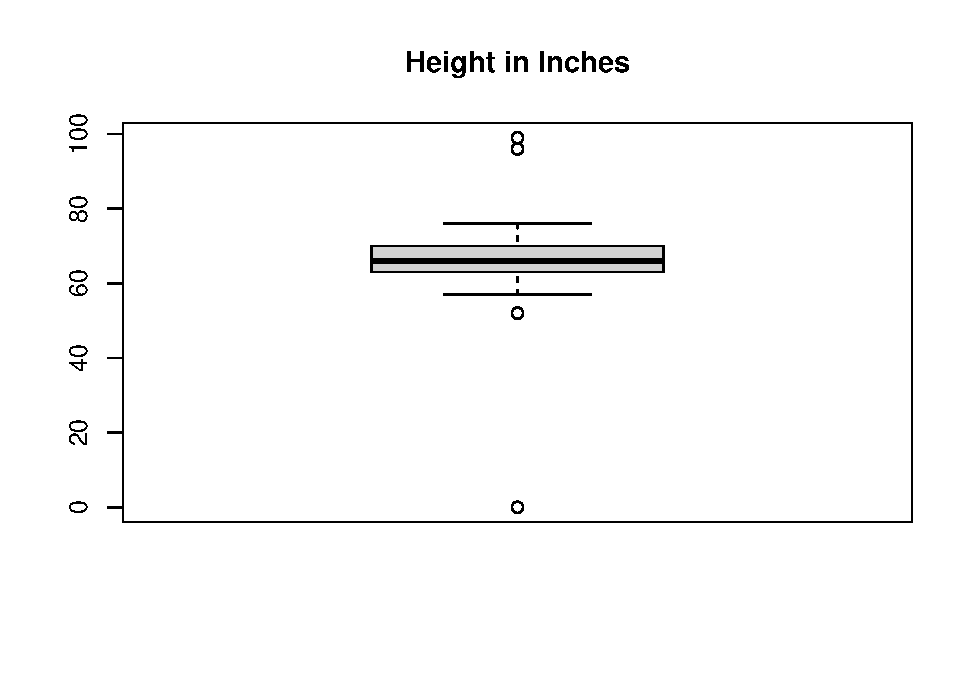
\includegraphics{_main_files/figure-latex/unnamed-chunk-14-1.pdf}

In this case, the values of 0, 95,96,97,98,99 all represent special coded values. \texttt{0} Indicates someone Not In Universe - someone for whom this question wasn't asked. This may be an infant too young to meaningfully be measured. In this case higher values represent a value of \texttt{unknown} for various reasons. Both of these values represent missing data, but they mean different things.

\begin{quote}
Why do you think we have more than one value to represent missing data? How does a value of 0 compare to a value of 99??
\end{quote}

We may want to exclude these special cases from our analysis. We can easily perform a data modification by filtering out values that equal any of our special cases. You can see the \textbf{range} of the graph is smaller, though visually, the box and whiskers are larger. Do we still see outliers in height?

\begin{Shaded}
\begin{Highlighting}[]
\FunctionTok{library}\NormalTok{(dplyr)}
\end{Highlighting}
\end{Shaded}

\begin{verbatim}
## 
## Attaching package: 'dplyr'
\end{verbatim}

\begin{verbatim}
## The following objects are masked from 'package:stats':
## 
##     filter, lag
\end{verbatim}

\begin{verbatim}
## The following objects are masked from 'package:base':
## 
##     intersect, setdiff, setequal, union
\end{verbatim}

\begin{Shaded}
\begin{Highlighting}[]
\NormalTok{new\_data }\OtherTok{\textless{}{-}}\NormalTok{ my\_data }\SpecialCharTok{\%\textgreater{}\%} \FunctionTok{filter}\NormalTok{(HEIGHT }\SpecialCharTok{\textgreater{}} \DecValTok{0} \SpecialCharTok{\&}\NormalTok{ HEIGHT }\SpecialCharTok{\textless{}} \DecValTok{95}\NormalTok{)}
\FunctionTok{boxplot}\NormalTok{(new\_data}\SpecialCharTok{$}\NormalTok{HEIGHT)}
\end{Highlighting}
\end{Shaded}

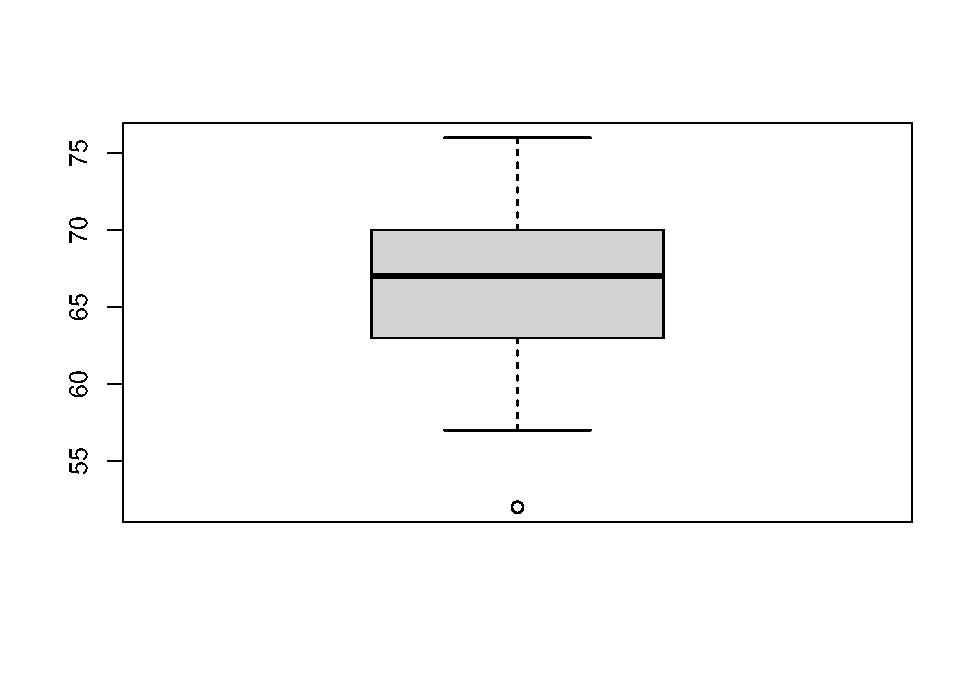
\includegraphics{_main_files/figure-latex/height_boxplot-1.pdf}

\hypertarget{elaborate}{%
\section{Elaborate}\label{elaborate}}

\hypertarget{your-turn}{%
\subsection{Your Turn!}\label{your-turn}}

For this example, you can use data collected in class, or the example dataset available in \texttt{ipumsED} R package: \texttt{class\_ipums\_data}

For in-class \emph{survey} data, you are looking at the age of each individual in class.
For the IPUMS data, you are looking at age as recorded in the American Community Survey
(\href{https://www.census.gov/programs-surveys/acs}{ACS}). This survey is fielded
annually. It contains more detailed questions that supplement the decennial census. \textbf{Raw data} are available directly from the \href{https://www.census.gov/programs-surveys/acs/data.html}{US Census Bureau}. However, we will be working with \href{https://ipums.org}{IPUMS data}, \textbf{harmonzied.}. This process standardizes variable coding schema across all samples within the IPUMS dataset. IPUMS makes it easy for researchers to conduct analysis across time and space.

\begin{quote}
IPUMS began as a PhD project digitizing historic US census data and reconciling
it with the coding schema of the current US Census (1990s). IPUMS-International grew out
of this by employing our harmonization practices on Census samples from other countries.
IPUMS has partnerships with over 100 countries and is working on building partnerships with the
remainng \textbf{82} countries!

Partnerships with IPUMS may look slightly different for each country, but they always
involve IPUMS commitment to being responsible stewards of the partner-country's data.
Our goal is to make data as open as possible, while maintaining responsible disclosure risk controls.
\end{quote}

Example data used throughout this book come from IPUMS-International so that values may be contextualized for a readers interested in one of the 103 countries that have data sharing agreements with IPUMS.

Write and \texttt{Rscript} that reads in your chosen dataset, and calculates the
following statistics:

\begin{itemize}
\tightlist
\item
  \texttt{mean()}
\item
  \texttt{meadian()}
\item
  \texttt{mode}
\item
  \texttt{range()}
\end{itemize}

In addition, include at least one plot or table and use it to discuss if your dataset contains any outliers. What criteria are you using to define an outlier?

\begin{quote}
Where's the \texttt{mode()}?? As a statistical programing language, R was developed with
built-in functions for \texttt{mean()}, \texttt{median()}, and \texttt{range()}. But \texttt{mode} wasn't important
enough to warrant its own function. In part, because it's so easy to code, even you
can do it!

Yep, we're serious!
\end{quote}

\hypertarget{evaluateexercises}{%
\section{Evaluate/Exercises}\label{evaluateexercises}}

\hypertarget{context}{%
\subsection{Context:}\label{context}}

Using the data set from Section 1.4 and the R statistics you produced,
answer the following questions about our data set.

\hypertarget{questions}{%
\subsection{Questions:}\label{questions}}

\textbf{Are the data quantitative or nominal?}

\emph{Click to show answer}

\begin{quote}
Age data is quantitative.
\end{quote}

\textbf{Are the data discrete or continuous?}

\emph{Click to show answer}

\begin{quote}
Age data is could be continuous depending on how you measure and record it,
but the way we generally talk about `Years of Age' is actually discrete.
\end{quote}

\textbf{Is the dataset primary or secondary data?}

\emph{Click to show answer}

\begin{quote}
That depends on which data you are using. If it was collected in your class, it is primary data. If you are using the IPUMS data, it is secondary data as the information was collected by IPUMS from the US Census.
\end{quote}

\textbf{What sampling method was used?}

\emph{Click to show answer}

\begin{quote}
Age data is quantitative.
\end{quote}

\textbf{Does any statistical bias exist?}

\emph{Click to show answer}

\begin{quote}
Age data is quantitative.
\end{quote}

\textbf{Which measure of central tendency is best to describe this data? Mean, Median or Mode.}

\emph{Click to show answer}

\begin{quote}
Age data is quantitative.
\end{quote}

\hypertarget{glossary}{%
\section{GLOSSARY}\label{glossary}}

Quantitative Data
Discrete Data
Continuous data:
Nominal Data:
Ordinal Data:
Primary Data:
Secondary Data:
Data Set:
Observation:
Variable:
Random Sampling:
Stratified Random Sampling:
Statistical Bias:
Mean:
Median:
Mode:
Range:
Outlier:
Statistic:
Sample Size:

\hypertarget{additional-content}{%
\section{Additional Content}\label{additional-content}}

\hypertarget{examples-from-recent-academic-articles}{%
\subsubsection{examples from recent academic articles}\label{examples-from-recent-academic-articles}}

article graphs, citations, instructors research, etc

\hypertarget{examples-from-non-academic}{%
\subsubsection{examples from non-academic}\label{examples-from-non-academic}}

customer satisfaction; workplace/department culture; r\&D;

\hypertarget{visualizing-data}{%
\chapter{Visualizing Data}\label{visualizing-data}}

\textbf{CURRENTLY JUST A COPY OF THE OLD 1.2, what is R; needs to be updated }

\hypertarget{engage-1}{%
\section{Engage}\label{engage-1}}

\textbf{Which visualization best represents the data?}

\textbf{Are there any problems with the visualizations?}

\hypertarget{vis-1}{%
\subsection{Vis 1}\label{vis-1}}

\emph{Click to show answer}

\begin{quote}
Barplots tend to be good choices to represent categorical data. They categories can be visualized side-by-side or stacked.
\end{quote}

.pull-left{[}

\begin{Shaded}
\begin{Highlighting}[]
\FunctionTok{barplot}\NormalTok{(}\FunctionTok{table}\NormalTok{(ff\_sex))}
\end{Highlighting}
\end{Shaded}

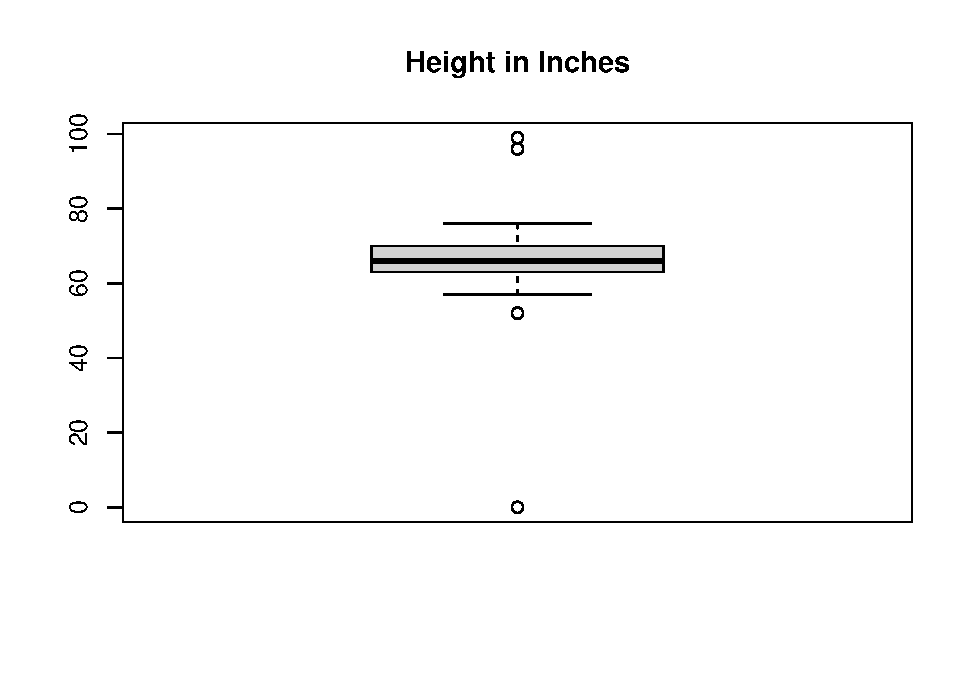
\includegraphics{_main_files/figure-latex/unnamed-chunk-16-1.pdf}
{]}

.pull-right{[}

\begin{Shaded}
\begin{Highlighting}[]
\FunctionTok{barplot}\NormalTok{(}\FunctionTok{table}\NormalTok{(ipums\_data}\SpecialCharTok{$}\NormalTok{AGE))}
\end{Highlighting}
\end{Shaded}

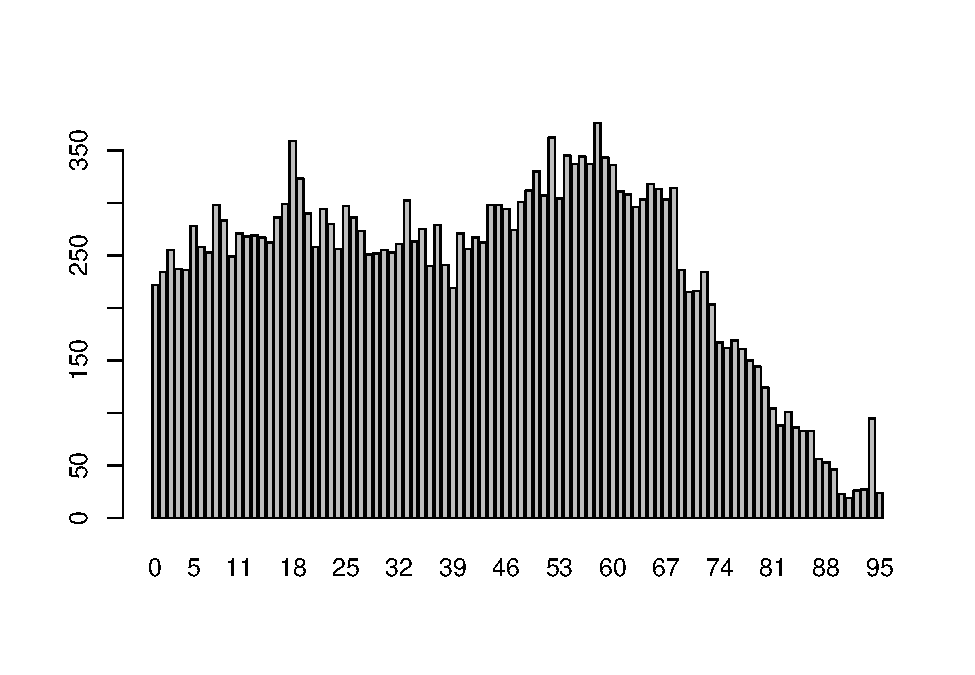
\includegraphics{_main_files/figure-latex/unnamed-chunk-17-1.pdf}

{]}

\hypertarget{vis-2}{%
\subsection{Vis 2}\label{vis-2}}

\begin{Shaded}
\begin{Highlighting}[]
\FunctionTok{plot}\NormalTok{(ff\_sex, }\AttributeTok{beside =} \ConstantTok{FALSE}\NormalTok{)}
\end{Highlighting}
\end{Shaded}

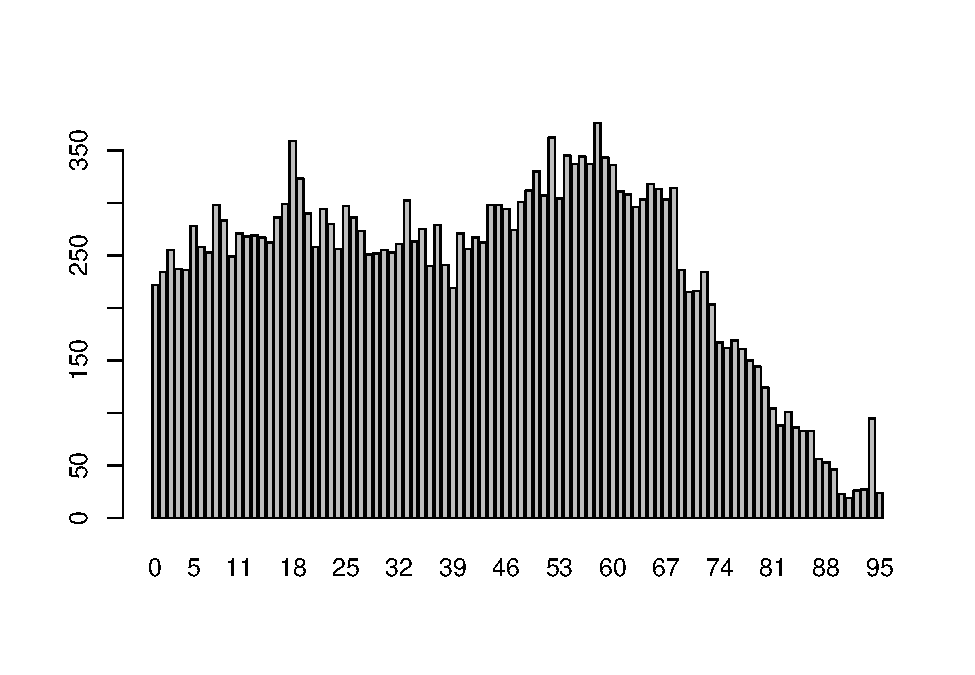
\includegraphics{_main_files/figure-latex/unnamed-chunk-18-1.pdf}

\hypertarget{vis-3}{%
\subsection{Vis 3}\label{vis-3}}

\begin{Shaded}
\begin{Highlighting}[]
\FunctionTok{table}\NormalTok{(ff\_marst)}
\end{Highlighting}
\end{Shaded}

\begin{verbatim}
## ff_marst
##    Single   Married Separated   Widowed 
##      9452      9688      2394      1313
\end{verbatim}

\begin{Shaded}
\begin{Highlighting}[]
\FunctionTok{round}\NormalTok{(}\FunctionTok{prop.table}\NormalTok{(}\FunctionTok{table}\NormalTok{(ff\_marst)),}\DecValTok{2}\NormalTok{)}
\end{Highlighting}
\end{Shaded}

\begin{verbatim}
## ff_marst
##    Single   Married Separated   Widowed 
##      0.41      0.42      0.10      0.06
\end{verbatim}

\hypertarget{explore-1}{%
\section{Explore}\label{explore-1}}

What do you want it to show vs what it shows. Maybe find a real data image from news that is clearly not good visualization

\hypertarget{explain-1}{%
\section{Explain}\label{explain-1}}

\emph{this section should mostly describe, examples will come in elaborate}

Visualizing data is the process of crafting a visual argument. All data visualizations require some level of subjective decsion making. Therefore any graph or table has some level of inherent bias. Effective data visualization involves crafting a visual argument, often one that conveys a direct story to the viewer.

As responsible researchers, educators, and data analysts we have a responsiblility to carefully consider our visual arguments.

An effective \textbf{and responsible} data visualization will lay out all relevant information (within reason), providing all the information for the reader to understand and build the visual argument for themselves.

\hypertarget{single-variable---continuous}{%
\subsection{Single Variable - Continuous}\label{single-variable---continuous}}

In general, your choice of visualization will depend on the \textbf{data type} that you are interested in. Continuous variables often get visually summarized using histograms, or box and whisker plots. These plots all serve to visually summarize the distrubtion and skew of a continuous variable.

\begin{itemize}
\tightlist
\item
  Continuous

  \begin{itemize}
  \tightlist
  \item
    Histogram
  \item
    Box Plot
  \item
    Summary Tables
  \item
    plot by index - \emph{example of not so helpful}
  \end{itemize}
\end{itemize}

\hypertarget{single-variable---categorical}{%
\subsection{Single Variable - Categorical}\label{single-variable---categorical}}

Categorical variables, are often better visualized using bar graphs, pie charts, or other \textbf{quantity/count plots}.

\begin{itemize}
\tightlist
\item
  Categorical

  \begin{itemize}
  \tightlist
  \item
    bar graphs
  \item
    pie charts
  \item
    freq/prop tables
  \end{itemize}
\end{itemize}

\hypertarget{multi-variable---continuous}{%
\subsection{Multi variable - continuous}\label{multi-variable---continuous}}

\begin{itemize}
\tightlist
\item
  scatter plots
\item
  line graphs
\item
  Cross Tabs
\end{itemize}

\hypertarget{mutli-variable---mixed}{%
\subsection{Mutli variable - mixed}\label{mutli-variable---mixed}}

\begin{itemize}
\tightlist
\item
  continuous \textasciitilde{} categorical

  \begin{itemize}
  \tightlist
  \item
    series of boxplots
  \end{itemize}
\item
  categorical \textasciitilde{} categorical

  \begin{itemize}
  \tightlist
  \item
    \emph{does this exist??}
  \end{itemize}
\item
  categorical \textasciitilde{} continuous

  \begin{itemize}
  \tightlist
  \item
    logistic regression - kind of
  \end{itemize}
\end{itemize}

\hypertarget{data-tables}{%
\subsection{Data Tables}\label{data-tables}}

\textbf{This could go into the R section}

\hypertarget{elaborate-1}{%
\section{Elaborate}\label{elaborate-1}}

In the next sections we will demonstrate some common visualzation using R. We will highlight common misteps and tips and tricks along the way. For each function we encourage you to try to come up with the syntax on your own, but you can click the \texttt{code} button to see how to generate the plots.

\hypertarget{making-visualizations-in-r}{%
\subsection{Making visualizations in R}\label{making-visualizations-in-r}}

\hypertarget{boxplot}{%
\subsubsection{Boxplot}\label{boxplot}}

Boxplots provide a great way to understand the distribution of the data at a glance. Three-quarters of the data are represented within the box portion of the plot. The full range of the data represented by the fences at the end of the vertical lines.

If there is an extreme range in the data, individual values will be plotted for the most extreme (3\% of)

\hypertarget{visualizations}{%
\paragraph{Visualizations}\label{visualizations}}

\begin{Shaded}
\begin{Highlighting}[]
\FunctionTok{boxplot}\NormalTok{(ipums\_data}\SpecialCharTok{$}\NormalTok{AGE)}
\end{Highlighting}
\end{Shaded}

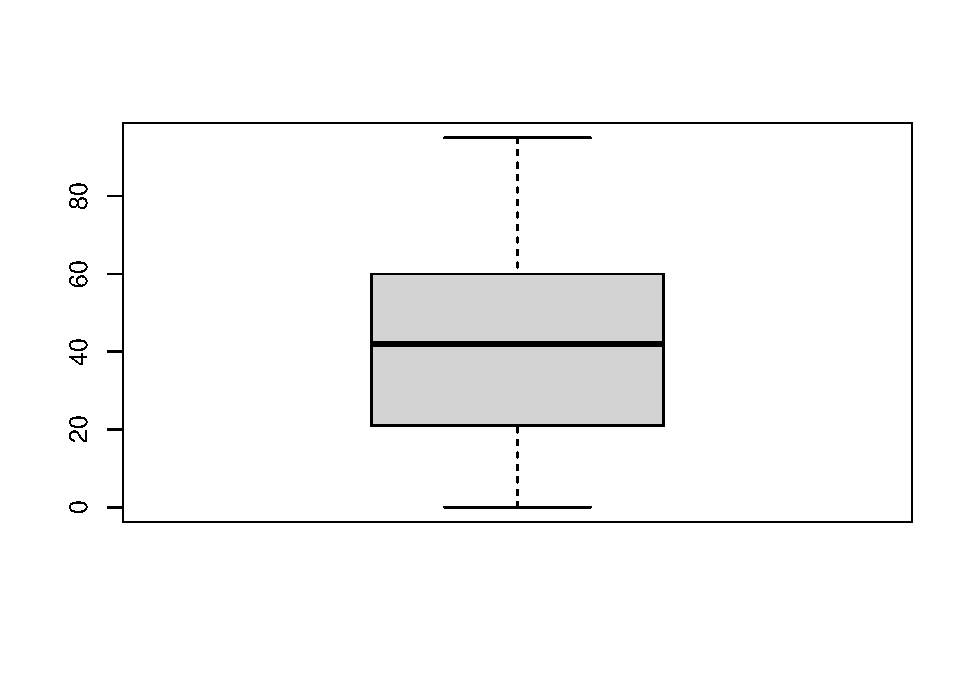
\includegraphics{_main_files/figure-latex/unnamed-chunk-20-1.pdf}

\hypertarget{summary-tables}{%
\paragraph{Summary Tables}\label{summary-tables}}

The \texttt{summary()} function can be applied to many data types. When applying to a continuous variable, it will returns a \textbf{5-number summary} along with the \textbf{mean}.

\textbf{Which numbers are included in the 5-number summary? How do these values relate to the box plot?}

\emph{Click to show answer}

\begin{quote}
The 5-number summary describes a dataset by providing the minimum, maximum, and median values. In a addition, the lower and upper quartiles are returned.

These 5 numbers represent key points on the boxplot. The extent of whiskers (minimum and maximum), the extent of the box (lower quartile and upper quartile), and the median.
\end{quote}

\begin{Shaded}
\begin{Highlighting}[]
\FunctionTok{summary}\NormalTok{(ipums\_data}\SpecialCharTok{$}\NormalTok{AGE)}
\end{Highlighting}
\end{Shaded}

\begin{verbatim}
##    Min. 1st Qu.  Median    Mean 3rd Qu.    Max. 
##    0.00   21.00   42.00   41.17   60.00   95.00
\end{verbatim}

\hypertarget{histograms}{%
\subsubsection{Histograms}\label{histograms}}

Histograms divide a continuous variable into several \texttt{bins}.

Try out the \texttt{hist()} function on a continuous varible like \texttt{AGE}.

\hypertarget{visualizations-1}{%
\paragraph{Visualizations}\label{visualizations-1}}

\begin{Shaded}
\begin{Highlighting}[]
\FunctionTok{hist}\NormalTok{(ipums\_data}\SpecialCharTok{$}\NormalTok{AGE)}
\end{Highlighting}
\end{Shaded}

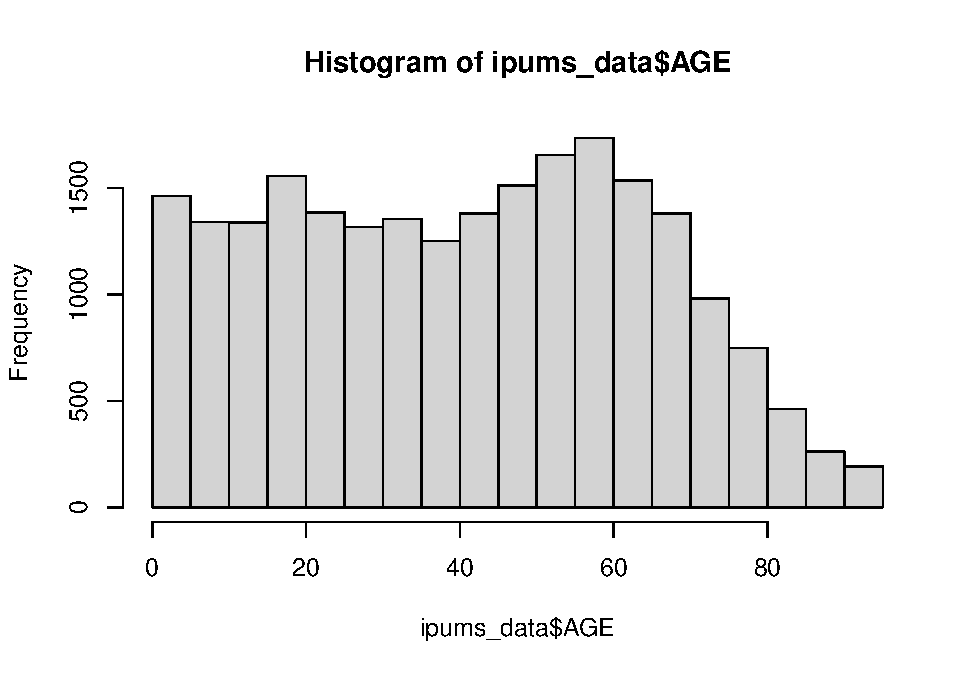
\includegraphics{_main_files/figure-latex/unnamed-chunk-22-1.pdf}

\hypertarget{summary-tables-1}{%
\paragraph{Summary Tables}\label{summary-tables-1}}

The same summary information applies to histograms.

\hypertarget{bar-chart}{%
\subsubsection{Bar Chart}\label{bar-chart}}

\hypertarget{visualizations-2}{%
\paragraph{Visualizations}\label{visualizations-2}}

\begin{Shaded}
\begin{Highlighting}[]
\FunctionTok{class}\NormalTok{(ipums\_data}\SpecialCharTok{$}\NormalTok{SEX)}
\end{Highlighting}
\end{Shaded}

\begin{verbatim}
## [1] "integer"
\end{verbatim}

\begin{Shaded}
\begin{Highlighting}[]
\FunctionTok{barplot}\NormalTok{(}\FunctionTok{table}\NormalTok{(ipums\_data}\SpecialCharTok{$}\NormalTok{SEX))}
\end{Highlighting}
\end{Shaded}

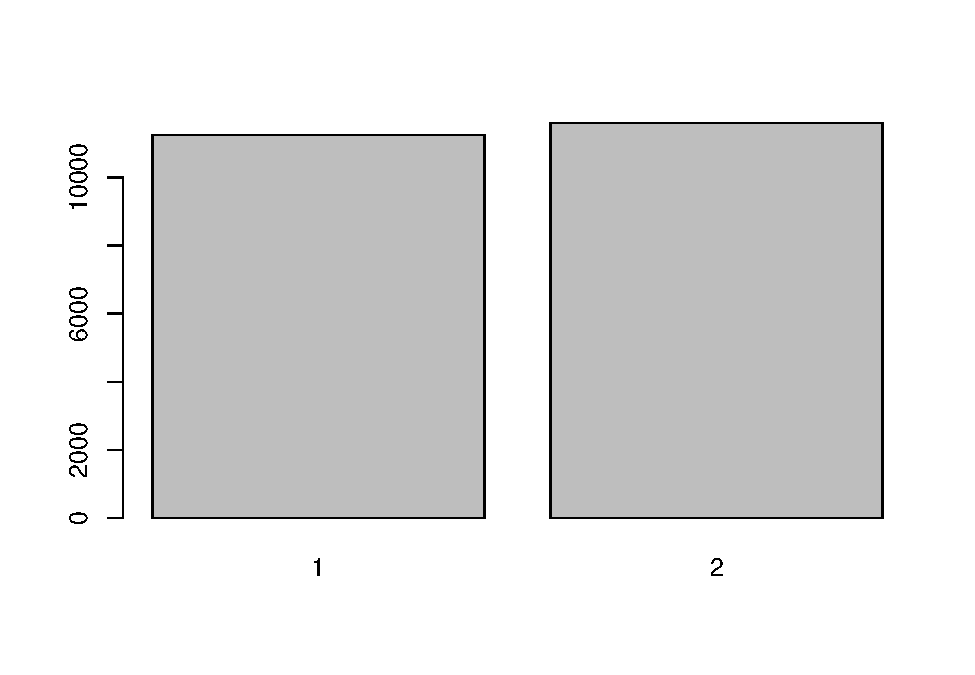
\includegraphics{_main_files/figure-latex/unnamed-chunk-23-1.pdf}

\hypertarget{summary-tables-2}{%
\paragraph{Summary Tables}\label{summary-tables-2}}

\hypertarget{pie-charts}{%
\subsubsection{Pie Charts}\label{pie-charts}}

\hypertarget{visualizations-3}{%
\paragraph{Visualizations}\label{visualizations-3}}

\hypertarget{summary-tables-3}{%
\paragraph{Summary Tables}\label{summary-tables-3}}

\hypertarget{scatter-plots}{%
\subsubsection{Scatter Plots}\label{scatter-plots}}

\hypertarget{visualizations-4}{%
\paragraph{Visualizations}\label{visualizations-4}}

\hypertarget{summary-tables-4}{%
\paragraph{Summary Tables}\label{summary-tables-4}}

\hypertarget{line-graphs}{%
\subsubsection{Line Graphs}\label{line-graphs}}

\hypertarget{visualizations-5}{%
\paragraph{Visualizations}\label{visualizations-5}}

\hypertarget{summary-tables-5}{%
\paragraph{Summary Tables}\label{summary-tables-5}}

\hypertarget{cross-tabs}{%
\subsubsection{Cross Tabs}\label{cross-tabs}}

\emph{can these be worked into the above sections?}

\textbf{Others\ldots{}}

\hypertarget{which-visualization-is-best-for-my-data-things-to-consider}{%
\subsection{Which visualization is best for my data? Things to consider}\label{which-visualization-is-best-for-my-data-things-to-consider}}

List things to consider for a visualization

\hypertarget{evaluateexercises-1}{%
\section{Evaluate/Exercises}\label{evaluateexercises-1}}

Give them a data set and have them think through why they choose a specific visualization. Have the create and answer questions about it.
We will go through the list of possible visualizations for the same data and explain which work, which dont, and why

\hypertarget{describing-data}{%
\chapter{Describing Data}\label{describing-data}}

\textbf{see old\_ for some examples, not very exstenive}

\hypertarget{engage-2}{%
\section{Engage}\label{engage-2}}

post-it note histogram of height:
* one with MANY bins
* one with FEW bins
* \emph{do these graphs tell the same story??}

\hypertarget{explore-2}{%
\section{Explore}\label{explore-2}}

How do we describe this meaningfully??
can we determine the ``average''

have class guess at average (likely the heighest point of histo)
* Interrogating a commonly held assumption
+ the average height of humans is 5'5''

Pose questions to explore

what does ``average'' mean??

\hypertarget{explain---lectureread}{%
\section{Explain - lecture/read}\label{explain---lectureread}}

\hypertarget{how-do-we-describe-data---summary-statistics}{%
\subsection{How do we describe data - summary statistics}\label{how-do-we-describe-data---summary-statistics}}

\hypertarget{how-do-we-describe-the-distribution-of-data}{%
\subsection{How do we describe the distribution of data}\label{how-do-we-describe-the-distribution-of-data}}

\hypertarget{how-do-we-manipulate-data}{%
\subsection{How do we manipulate data}\label{how-do-we-manipulate-data}}

\hypertarget{codingcategorizing-free-response-binning-a-continuous-variable}{%
\subsubsection{coding/categorizing free response/ ``binning'' a continuous variable}\label{codingcategorizing-free-response-binning-a-continuous-variable}}

Height, while we treat as continuous, is actually ``binned'' into \textasciitilde60 unique values.

\hypertarget{normality}{%
\section{Normality}\label{normality}}

What does it mean to be normally distributed. (how measures of central tendency compare)
discuss skew / kurtosis
specialized vocabulary to describe data
Why people care about normality (what tests can/t you use and why)

\hypertarget{elaborate-2}{%
\section{Elaborate}\label{elaborate-2}}

Read/write data
Visualize data - describe the distribution; compare to board results
Tabulate Data - describe with summary statistics
Test of normality: one-way t-test ; QQ plot ; shapiro-wilks (note high rate of rejection)
Demo binnig of ages

\hypertarget{evaluateexercises-2}{%
\section{Evaluate/Exercises}\label{evaluateexercises-2}}

Write an R script that:
1. reads in data
1. tests normality across variables
1. print results as table
1. prints results as graph.

Reflect: Are any variables non-normal? Do you have any interpretations as to why?
Do you have any questions to test

\hypertarget{hypothesis-testing---comparison-and-correlations}{%
\chapter{Hypothesis Testing - Comparison and Correlations}\label{hypothesis-testing---comparison-and-correlations}}

\hypertarget{engage-3}{%
\section{Engage}\label{engage-3}}

Post-it histogram - height separated by birth month (may require a lot of board space)

Are the distributions similar? different? \textbf{too many small samples to tell}?

\hypertarget{explore-3}{%
\section{Explore}\label{explore-3}}

How do we \textbf{group} data in order to compare it.

The most simple question in statisitics is:
Is x bigger than y

How can we do that for our groups here?

Summer/Winter?

conduct demo/small-scale experiment/analysis
Ask leading questions, form hypotheses;
* can the example be grouped / broken into subgroups
+ does the same pattern/phenomenon apply?
* Is there a corollary / inverse phenomenon?

Pose questions to explore

Discuss/interrogate the pattern of the data
* does the shape imply anything
* try to have it student led / guided
* with time, students guess at what the data shows/doesn't show without labels

\hypertarget{explain---lectureread-1}{%
\section{Explain - lecture/read}\label{explain---lectureread-1}}

demo recode: birth month -\textgreater{} Summer/Winter (daylight-savings or not);
recode favorite food to sweet/savory

\hypertarget{why-2-groups}{%
\subsection{Why 2 groups?}\label{why-2-groups}}

Historical problem of statistics. We've developed very good methods for very un-reasonable
situations. In order to make these tests work, we often have to \textbf{manipulate}
our data in order to meet the \textbf{assumptions} of the specific test or analysis
that we'd like to perform.

\hypertarget{common-tests-to-compare-2-groups}{%
\subsection{Common tests to compare 2 groups}\label{common-tests-to-compare-2-groups}}

t-test and chisq \textbar{} box-whisker, histogram, density distribution

\hypertarget{correlations}{%
\subsection{Correlation(s)}\label{correlations}}

correlation (pearson, spearman) \textbar{} scatter plot
height \textasciitilde{} hrs\_slept ; height \textasciitilde{} fav\_food\_category

\hypertarget{elaborate-3}{%
\section{Elaborate}\label{elaborate-3}}

demo recode: birth month -\textgreater{} Summer/Winter (daylight-savings or not); recode favorite food to sweet/savory
t-test and chisq \textbar{} box-whisker, histogram, density distribution
height \textasciitilde{} birth\_SW
correlation (pearson, spearman) \textbar{} scatter plot
height \textasciitilde{} hrs\_slept ; height \textasciitilde{} fav\_food\_category
What is an hypothesis??

\hypertarget{evaluateexercises-3}{%
\section{Evaluate/Exercises}\label{evaluateexercises-3}}

Formulate a hypothesis and test it using class survey data.
Recode birth month to birth\_quarter; recode favorite food to 3 or more categories

\hypertarget{hypothesis-testing---anova-and-lm}{%
\chapter{Hypothesis Testing - ANOVA and LM}\label{hypothesis-testing---anova-and-lm}}

\hypertarget{engage-4}{%
\section{Engage}\label{engage-4}}

Compare MORE than 2 groups

Post-it histogram - height separated by Birth Mo (reclassified to birth quarter)

\hypertarget{explore-4}{%
\section{Explore}\label{explore-4}}

Pose questions to explore

Are the four distributions similar? different?

\hypertarget{explain---lectureread-2}{%
\section{Explain - lecture/read}\label{explain---lectureread-2}}

What is ANOVA, how to interpret tabularly, graphically (box-whisker, histo, density); non-parametric alternative (KS)
What is a linear model? LM vs Correlation vs ANOVA
What does a linear relationship imply?
LM = continuous \textasciitilde{} continuous
ANOVA = continuous \textasciitilde{} categorical

\hypertarget{elaborate-4}{%
\section{Elaborate}\label{elaborate-4}}

Conduct recoding for birth quarter
conduct ANOVA
Conduct Linear Model

Work through the same process/analysis on new data. Either a different
variable(s) in the same sample, or applying/demonstrating the phenomenon
using real-world data/examples.

\begin{itemize}
\tightlist
\item
  Reiterate/reinforc the process/task of the lesson
\item
  Does this fit in to other steps/analysis
\item
  does this fit in to other thematic topics?
\end{itemize}

(Possibly) Build on the first one to show variation.
* Other ways to represent the phenomenon/data
+ tabular
+ visually

\hypertarget{evaluateexercises-4}{%
\section{Evaluate/Exercises}\label{evaluateexercises-4}}

Formulate a hypothesis and test it using class survey data.

\hypertarget{unit-2-ipums}{%
\chapter*{Unit 2: IPUMS}\label{unit-2-ipums}}
\addcontentsline{toc}{chapter}{Unit 2: IPUMS}

\hypertarget{lesson-6-introduction-to-ipums}{%
\section*{Lesson 6 Introduction to IPUMS}\label{lesson-6-introduction-to-ipums}}

Some text to break up the sub-section headers

\hypertarget{intro-to-ipums-website}{%
\subsection*{Intro to IPUMS website}\label{intro-to-ipums-website}}
\addcontentsline{toc}{subsection}{Intro to IPUMS website}

\hypertarget{background-on-ipums}{%
\subsection*{background on ipums}\label{background-on-ipums}}
\addcontentsline{toc}{subsection}{background on ipums}

\hypertarget{navigating-website}{%
\subsection*{navigating website}\label{navigating-website}}
\addcontentsline{toc}{subsection}{navigating website}

Find certain (very common) variables to answer (common) social science questions.

\hypertarget{lesson-7-exploratory-analysis}{%
\section*{Lesson 7 Exploratory analysis}\label{lesson-7-exploratory-analysis}}

If you've just collected a survey, or other raw data, you may not know what you're looking for. This is perfectly ok but goes against \emph{the scientific method} most people learned in grade school (More on that to follow(\textbf{\emph{include\_link}})).

This unit begins by presenting data/distributions and asking students to begin interpreting the data . visual exploration is encouraged and basic of data manipulation are taught
* \emph{EG:} how to subset data, how to reshape data, how to recode data, how to convert from one \texttt{data\ type} to another.

Example lab exercise:

Students given a data set (xls, csv, etc)
* load data, perform manipulations, basic summaries
+ cross tabs
+ group means by a covariate
* inspect data visually
+ \emph{DESCRIBE} the distribution - is it normal? significant?
* \emph{FIND} aquestion in the spread of the data
+ how can you test this (maybe small group work)
* write up/ present results
+ think on confounding factors / biases

\hypertarget{advanced-exploration---change-over-time}{%
\subsection*{Advanced Exploration - Change Over Time}\label{advanced-exploration---change-over-time}}
\addcontentsline{toc}{subsection}{Advanced Exploration - Change Over Time}

Here we demonstrate an approach to looking at how Family Structure (inferred from household relationships) has changed over time.

\hypertarget{setup-load-data}{%
\subsubsection*{Setup / Load Data}\label{setup-load-data}}
\addcontentsline{toc}{subsubsection}{Setup / Load Data}

Install/update R packages

\begin{Shaded}
\begin{Highlighting}[]
\FunctionTok{install.packages}\NormalTok{(}\StringTok{"ipumsr"}\NormalTok{)}
\FunctionTok{install.packages}\NormalTok{(}\StringTok{"tidyverse"}\NormalTok{)}
\end{Highlighting}
\end{Shaded}

Data extract created online using the datacart system.

\begin{Shaded}
\begin{Highlighting}[]
\FunctionTok{library}\NormalTok{(ipumsr)}
\FunctionTok{library}\NormalTok{(dplyr)}


\NormalTok{ddi }\OtherTok{\textless{}{-}} \FunctionTok{read\_ipums\_ddi}\NormalTok{(}\StringTok{"Data/ipumsi\_00005.xml"}\NormalTok{)}
\NormalTok{data }\OtherTok{\textless{}{-}} \FunctionTok{read\_ipums\_micro}\NormalTok{(ddi)}
\end{Highlighting}
\end{Shaded}

\hypertarget{inspect-the-data}{%
\paragraph*{Inspect the Data}\label{inspect-the-data}}
\addcontentsline{toc}{paragraph}{Inspect the Data}

Using \texttt{haven} labeled values.

\begin{Shaded}
\begin{Highlighting}[]
\NormalTok{data}\SpecialCharTok{$}\NormalTok{RELATE[}\DecValTok{1}\SpecialCharTok{:}\DecValTok{100}\NormalTok{]}
\FunctionTok{class}\NormalTok{(data}\SpecialCharTok{$}\NormalTok{RELATE)}

\NormalTok{data }\SpecialCharTok{\%\textgreater{}\%} \FunctionTok{count}\NormalTok{(RELATE)}
\NormalTok{data }\SpecialCharTok{\%\textgreater{}\%} \FunctionTok{count}\NormalTok{(SEX)}
\end{Highlighting}
\end{Shaded}

What were those codes ??

\begin{Shaded}
\begin{Highlighting}[]
\DocumentationTok{\#\# need to convert this to an image or something similar; kable table?}
\FunctionTok{ipums\_view}\NormalTok{(ddi)}
\end{Highlighting}
\end{Shaded}

\hypertarget{visualize}{%
\paragraph*{Visualize}\label{visualize}}
\addcontentsline{toc}{paragraph}{Visualize}

A simple plot

\begin{Shaded}
\begin{Highlighting}[]
\FunctionTok{plot}\NormalTok{(AGE }\SpecialCharTok{\textasciitilde{}}\NormalTok{ YEAR, }\AttributeTok{data =}\NormalTok{ data)}
\end{Highlighting}
\end{Shaded}

A fancier plot

\begin{Shaded}
\begin{Highlighting}[]
\FunctionTok{plot}\NormalTok{(AGE}\SpecialCharTok{\textasciitilde{}}\NormalTok{YEAR, }\AttributeTok{data =}\NormalTok{ data, }\AttributeTok{type =} \StringTok{"n"}\NormalTok{, }\AttributeTok{main =} \StringTok{"Age by Sex, over Time, CO"}\NormalTok{)}
\FunctionTok{points}\NormalTok{(data}\SpecialCharTok{$}\NormalTok{YEAR[data}\SpecialCharTok{$}\NormalTok{SEX}\SpecialCharTok{==}\DecValTok{1}\NormalTok{]}\SpecialCharTok{{-}}\DecValTok{1}\NormalTok{, data}\SpecialCharTok{$}\NormalTok{AGE[data}\SpecialCharTok{$}\NormalTok{SEX}\SpecialCharTok{==}\DecValTok{1}\NormalTok{], }\AttributeTok{pch =} \DecValTok{16}\NormalTok{, }\AttributeTok{col =} \FunctionTok{hsv}\NormalTok{(.}\DecValTok{6}\NormalTok{,.}\DecValTok{6}\NormalTok{,.}\DecValTok{8}\NormalTok{,.}\DecValTok{2}\NormalTok{))}

\FunctionTok{points}\NormalTok{(data}\SpecialCharTok{$}\NormalTok{YEAR[data}\SpecialCharTok{$}\NormalTok{SEX}\SpecialCharTok{==}\DecValTok{2}\NormalTok{]}\SpecialCharTok{+}\DecValTok{1}\NormalTok{, data}\SpecialCharTok{$}\NormalTok{AGE[data}\SpecialCharTok{$}\NormalTok{SEX}\SpecialCharTok{==}\DecValTok{2}\NormalTok{], }\AttributeTok{pch =} \DecValTok{16}\NormalTok{, }\AttributeTok{col =} \FunctionTok{hsv}\NormalTok{(}\DecValTok{1}\NormalTok{,.}\DecValTok{6}\NormalTok{,.}\DecValTok{8}\NormalTok{,.}\DecValTok{2}\NormalTok{))}

\FunctionTok{abline}\NormalTok{(}\FunctionTok{lm}\NormalTok{(AGE}\SpecialCharTok{\textasciitilde{}}\NormalTok{YEAR, }\AttributeTok{data =}\NormalTok{ data), }\AttributeTok{col =} \StringTok{"green"}\NormalTok{)}
\end{Highlighting}
\end{Shaded}

\hypertarget{asking-logical-questions}{%
\paragraph*{Asking (logical) questions}\label{asking-logical-questions}}
\addcontentsline{toc}{paragraph}{Asking (logical) questions}

Here we demonstrate how setting up logical questions can be used to easily filter/subset data.

\begin{Shaded}
\begin{Highlighting}[]
\NormalTok{age\_test }\OtherTok{\textless{}{-}}\NormalTok{ data}\SpecialCharTok{$}\NormalTok{AGE }\SpecialCharTok{\textgreater{}} \DecValTok{18}

\FunctionTok{class}\NormalTok{(age\_test)}

\NormalTok{age\_test}
\end{Highlighting}
\end{Shaded}

Logical vectors are stored as \texttt{TRUE} or \texttt{FALSE}, but can also be evaluated numerically as \texttt{1} or \texttt{0} respectively. We can therefore \texttt{sum()} the number of \texttt{TRUE} values and divide by total rows for a proportion.

\begin{Shaded}
\begin{Highlighting}[]
\FunctionTok{sum}\NormalTok{(age\_test)}\SpecialCharTok{/}\FunctionTok{nrow}\NormalTok{(data)}
\end{Highlighting}
\end{Shaded}

\hypertarget{hh-vs-persons}{%
\paragraph*{HH vs persons}\label{hh-vs-persons}}
\addcontentsline{toc}{paragraph}{HH vs persons}

A unique characteristic of census and some survey data is the nested-structure with individuals being grouped into households. Often times it is necessary to choose to work at the hh or person level, and data must be appropriately manipulated to fit that case.

\begin{Shaded}
\begin{Highlighting}[]
\NormalTok{hh\_total }\OtherTok{\textless{}{-}} \FunctionTok{length}\NormalTok{(}\FunctionTok{unique}\NormalTok{(data}\SpecialCharTok{$}\NormalTok{SERIAL))}
\NormalTok{hh\_total}
\FunctionTok{ipums\_view}\NormalTok{(ddi)}
\end{Highlighting}
\end{Shaded}

\hypertarget{nuclear-family}{%
\subsubsection*{Nuclear Family}\label{nuclear-family}}
\addcontentsline{toc}{subsubsection}{Nuclear Family}

First we look at a nuclear family, comprising only parents and their immediate children.

\begin{Shaded}
\begin{Highlighting}[]
\FunctionTok{library}\NormalTok{(ipumsr)}
\FunctionTok{library}\NormalTok{(dplyr)}

\NormalTok{ddi }\OtherTok{\textless{}{-}} \FunctionTok{read\_ipums\_ddi}\NormalTok{(}\StringTok{"/pkg/ipums/personal/ehrli097/AABA\_2022/Data/ipumsi\_00005.xml"}\NormalTok{)}
\NormalTok{all\_data }\OtherTok{\textless{}{-}} \FunctionTok{read\_ipums\_micro}\NormalTok{(ddi)}

\NormalTok{census\_years }\OtherTok{\textless{}{-}} \FunctionTok{c}\NormalTok{(}\DecValTok{1860}\NormalTok{, }\DecValTok{1870}\NormalTok{, }\DecValTok{1880}\NormalTok{, }\DecValTok{1900}\NormalTok{, }\DecValTok{1910}\NormalTok{, }\DecValTok{1960}\NormalTok{, }\DecValTok{1970}\NormalTok{, }\DecValTok{1980}\NormalTok{, }\DecValTok{1990}\NormalTok{, }\DecValTok{2000}\NormalTok{, }\DecValTok{2010}\NormalTok{)}

\DocumentationTok{\#\# subset census only}
\NormalTok{d2 }\OtherTok{\textless{}{-}}\NormalTok{ all\_data }\SpecialCharTok{\%\textgreater{}\%} \FunctionTok{filter}\NormalTok{(YEAR }\SpecialCharTok{\%in\%}\NormalTok{ census\_years)}

\DocumentationTok{\#\# make a household dataframe}
\NormalTok{hhs }\OtherTok{\textless{}{-}}\NormalTok{ d2 }\SpecialCharTok{\%\textgreater{}\%} \FunctionTok{distinct}\NormalTok{(YEAR, SERIAL, }\AttributeTok{.keep\_all =} \ConstantTok{TRUE}\NormalTok{) }\SpecialCharTok{\%\textgreater{}\%} \FunctionTok{select}\NormalTok{(YEAR,SERIAL,GEO1\_US)}

\NormalTok{hhs }\SpecialCharTok{\%\textgreater{}\%} \FunctionTok{View}\NormalTok{()}
\end{Highlighting}
\end{Shaded}

\begin{Shaded}
\begin{Highlighting}[]
\NormalTok{hhs }\OtherTok{\textless{}{-}}\NormalTok{ d2 }\SpecialCharTok{\%\textgreater{}\%} \FunctionTok{filter}\NormalTok{(RELATE }\SpecialCharTok{==}\DecValTok{4}\NormalTok{) }\SpecialCharTok{\%\textgreater{}\%} 
  
  
  \FunctionTok{distinct}\NormalTok{(YEAR, SERIAL) }\SpecialCharTok{\%\textgreater{}\%} \FunctionTok{mutate}\NormalTok{(}\AttributeTok{extended\_test=}\ConstantTok{TRUE}\NormalTok{) }\SpecialCharTok{\%\textgreater{}\%} \FunctionTok{right\_join}\NormalTok{(hhs, }\AttributeTok{by =} \FunctionTok{c}\NormalTok{(}\StringTok{"YEAR"}\NormalTok{, }\StringTok{"SERIAL"}\NormalTok{)) }\SpecialCharTok{\%\textgreater{}\%} \FunctionTok{mutate}\NormalTok{(}\AttributeTok{extended\_test=}\FunctionTok{if\_else}\NormalTok{(}\FunctionTok{is.na}\NormalTok{(extended\_test),}\ConstantTok{FALSE}\NormalTok{,}\ConstantTok{TRUE}\NormalTok{))}
  








\NormalTok{hhs }\OtherTok{\textless{}{-}}\NormalTok{ d2 }\SpecialCharTok{\%\textgreater{}\%} \FunctionTok{filter}\NormalTok{(}\SpecialCharTok{!}\NormalTok{RELATE }\SpecialCharTok{\%in\%} \FunctionTok{c}\NormalTok{(}\DecValTok{1}\NormalTok{, }\DecValTok{2}\NormalTok{, }\DecValTok{3}\NormalTok{) }\SpecialCharTok{|}
\NormalTok{                  (RELATE }\SpecialCharTok{==} \DecValTok{3} \SpecialCharTok{\&}
\NormalTok{                     MARST }\SpecialCharTok{\%in\%} \FunctionTok{c}\NormalTok{(}\DecValTok{2}\NormalTok{, }\DecValTok{3}\NormalTok{, }\DecValTok{4}\NormalTok{))}
\NormalTok{                ) }\SpecialCharTok{\%\textgreater{}\%} 

  
  
  \FunctionTok{distinct}\NormalTok{(YEAR, SERIAL) }\SpecialCharTok{\%\textgreater{}\%} \FunctionTok{mutate}\NormalTok{(}\AttributeTok{nuclear\_test =} \ConstantTok{FALSE}\NormalTok{) }\SpecialCharTok{\%\textgreater{}\%} \FunctionTok{right\_join}\NormalTok{(hhs, }\AttributeTok{by =} \FunctionTok{c}\NormalTok{(}\StringTok{"YEAR"}\NormalTok{, }\StringTok{"SERIAL"}\NormalTok{)) }\SpecialCharTok{\%\textgreater{}\%} \FunctionTok{mutate}\NormalTok{(}\AttributeTok{nuclear\_test =} \FunctionTok{if\_else}\NormalTok{(}\FunctionTok{is.na}\NormalTok{(nuclear\_test), }\ConstantTok{TRUE}\NormalTok{, }\ConstantTok{FALSE}\NormalTok{))}



\FunctionTok{table}\NormalTok{(hhs}\SpecialCharTok{$}\NormalTok{extended\_test,hhs}\SpecialCharTok{$}\NormalTok{nuclear\_test)}
\end{Highlighting}
\end{Shaded}

\hypertarget{tabulate-results}{%
\paragraph*{Tabulate results}\label{tabulate-results}}
\addcontentsline{toc}{paragraph}{Tabulate results}

\begin{Shaded}
\begin{Highlighting}[]
\NormalTok{  hhs }\OtherTok{\textless{}{-}}\NormalTok{ d2 }\SpecialCharTok{\%\textgreater{}\%} \FunctionTok{filter}\NormalTok{(RELATED }\SpecialCharTok{\%in\%} \FunctionTok{c}\NormalTok{(}\DecValTok{4200}\NormalTok{, }\DecValTok{4210}\NormalTok{, }\DecValTok{4211}\NormalTok{, }\DecValTok{4220}\NormalTok{, }\DecValTok{4500}\NormalTok{, }\DecValTok{4510}\NormalTok{, }\DecValTok{4600}\NormalTok{)) }\SpecialCharTok{\%\textgreater{}\%} \FunctionTok{distinct}\NormalTok{(YEAR, SERIAL) }\SpecialCharTok{\%\textgreater{}\%} \FunctionTok{mutate}\NormalTok{(}\AttributeTok{parent\_test=}\ConstantTok{TRUE}\NormalTok{) }\SpecialCharTok{\%\textgreater{}\%} \FunctionTok{right\_join}\NormalTok{(hhs, }\AttributeTok{by =} \FunctionTok{c}\NormalTok{(}\StringTok{"YEAR"}\NormalTok{, }\StringTok{"SERIAL"}\NormalTok{)) }\SpecialCharTok{\%\textgreater{}\%} \FunctionTok{mutate}\NormalTok{(}\AttributeTok{parent\_test=}\FunctionTok{if\_else}\NormalTok{(}\FunctionTok{is.na}\NormalTok{(parent\_test),}\ConstantTok{FALSE}\NormalTok{,}\ConstantTok{TRUE}\NormalTok{))}


\NormalTok{  hhs }\OtherTok{\textless{}{-}}\NormalTok{ d2 }\SpecialCharTok{\%\textgreater{}\%} \FunctionTok{filter}\NormalTok{(RELATED }\SpecialCharTok{\%in\%} \FunctionTok{c}\NormalTok{(}\DecValTok{4100}\NormalTok{, }\DecValTok{4110}\NormalTok{, }\DecValTok{4120}\NormalTok{, }\DecValTok{4130}\NormalTok{, }\DecValTok{4300}\NormalTok{, }\DecValTok{4301}\NormalTok{, }\DecValTok{4302}\NormalTok{)) }\SpecialCharTok{\%\textgreater{}\%} \FunctionTok{distinct}\NormalTok{(YEAR, SERIAL) }\SpecialCharTok{\%\textgreater{}\%} \FunctionTok{mutate}\NormalTok{(}\AttributeTok{children\_test=}\ConstantTok{TRUE}\NormalTok{) }\SpecialCharTok{\%\textgreater{}\%} \FunctionTok{right\_join}\NormalTok{(hhs, }\AttributeTok{by =} \FunctionTok{c}\NormalTok{(}\StringTok{"YEAR"}\NormalTok{, }\StringTok{"SERIAL"}\NormalTok{)) }\SpecialCharTok{\%\textgreater{}\%} \FunctionTok{mutate}\NormalTok{(}\AttributeTok{children\_test=}\FunctionTok{if\_else}\NormalTok{(}\FunctionTok{is.na}\NormalTok{(children\_test),}\ConstantTok{FALSE}\NormalTok{,}\ConstantTok{TRUE}\NormalTok{))}
  
  
\NormalTok{  res\_tabs }\OtherTok{\textless{}{-}} \FunctionTok{list}\NormalTok{(}
    \StringTok{"nuclear\_test"} \OtherTok{=}\NormalTok{ hhs }\SpecialCharTok{\%\textgreater{}\%} \FunctionTok{group\_by}\NormalTok{(YEAR, nuclear\_test,GEO1\_US) }\SpecialCharTok{\%\textgreater{}\%} \FunctionTok{summarize}\NormalTok{(}\AttributeTok{.groups=}\StringTok{"drop"}\NormalTok{,}\AttributeTok{n =} \FunctionTok{n}\NormalTok{()) }\SpecialCharTok{\%\textgreater{}\%} \FunctionTok{as.data.frame}\NormalTok{(),}
  \StringTok{"extended\_test"} \OtherTok{=}\NormalTok{ hhs }\SpecialCharTok{\%\textgreater{}\%} \FunctionTok{group\_by}\NormalTok{(YEAR, extended\_test, GEO1\_US) }\SpecialCharTok{\%\textgreater{}\%} \FunctionTok{summarize}\NormalTok{(}\AttributeTok{.groups=}\StringTok{"drop"}\NormalTok{,}\AttributeTok{n =} \FunctionTok{n}\NormalTok{()) }\SpecialCharTok{\%\textgreater{}\%} \FunctionTok{as.data.frame}\NormalTok{(),}
  \StringTok{"parent\_test"} \OtherTok{=}\NormalTok{ hhs }\SpecialCharTok{\%\textgreater{}\%} \FunctionTok{group\_by}\NormalTok{(YEAR, parent\_test, GEO1\_US) }\SpecialCharTok{\%\textgreater{}\%} \FunctionTok{summarize}\NormalTok{(}\AttributeTok{.groups=}\StringTok{"drop"}\NormalTok{,}\AttributeTok{n =} \FunctionTok{n}\NormalTok{()) }\SpecialCharTok{\%\textgreater{}\%} \FunctionTok{as.data.frame}\NormalTok{(),}
  \StringTok{"children\_test"} \OtherTok{=}\NormalTok{ hhs }\SpecialCharTok{\%\textgreater{}\%} \FunctionTok{group\_by}\NormalTok{(YEAR, children\_test, GEO1\_US) }\SpecialCharTok{\%\textgreater{}\%} \FunctionTok{summarize}\NormalTok{(}\AttributeTok{.groups=}\StringTok{"drop"}\NormalTok{,}\AttributeTok{n =} \FunctionTok{n}\NormalTok{()) }\SpecialCharTok{\%\textgreater{}\%} \FunctionTok{as.data.frame}\NormalTok{()}
\NormalTok{  )}
  
  
  
  

\NormalTok{collapsed\_results }\OtherTok{\textless{}{-}}\NormalTok{ res\_tabs }\SpecialCharTok{\%\textgreater{}\%}\NormalTok{ purrr}\SpecialCharTok{::}\FunctionTok{map}\NormalTok{(}\ControlFlowTok{function}\NormalTok{(x)\{}
\NormalTok{  x }\OtherTok{\textless{}{-}}\NormalTok{ x }\SpecialCharTok{\%\textgreater{}\%} \FunctionTok{group\_by}\NormalTok{(}\FunctionTok{across}\NormalTok{(}\FunctionTok{names}\NormalTok{(x)[}\DecValTok{1}\SpecialCharTok{:}\DecValTok{3}\NormalTok{])) }\SpecialCharTok{\%\textgreater{}\%} \FunctionTok{summarize}\NormalTok{(}\AttributeTok{.groups=}\StringTok{"drop"}\NormalTok{,}\AttributeTok{n =} \FunctionTok{sum}\NormalTok{(n))}

\NormalTok{\})}


\NormalTok{collapsed\_results }\OtherTok{\textless{}{-}} \FunctionTok{lapply}\NormalTok{(collapsed\_results, }\ControlFlowTok{function}\NormalTok{(x)\{}
  \FunctionTok{colnames}\NormalTok{(x)[}\DecValTok{2}\NormalTok{] }\OtherTok{\textless{}{-}} \StringTok{"test"}
  \FunctionTok{colnames}\NormalTok{(x)[}\DecValTok{3}\NormalTok{] }\OtherTok{\textless{}{-}} \StringTok{"state"}
  \FunctionTok{return}\NormalTok{(x)}
\NormalTok{\})}

\NormalTok{combined }\OtherTok{\textless{}{-}}\NormalTok{ collapsed\_results }\SpecialCharTok{\%\textgreater{}\%}\NormalTok{ purrr}\SpecialCharTok{::}\FunctionTok{reduce}\NormalTok{(full\_join, }\AttributeTok{by =} \FunctionTok{c}\NormalTok{(}\StringTok{"YEAR"}\NormalTok{, }\StringTok{"test"}\NormalTok{, }\StringTok{"state"}\NormalTok{))}



\FunctionTok{colnames}\NormalTok{(combined) }\OtherTok{\textless{}{-}} \FunctionTok{c}\NormalTok{(}\StringTok{"YEAR"}\NormalTok{,}\StringTok{"test"}\NormalTok{, }\StringTok{"state"}\NormalTok{, }\StringTok{"n\_nuclear"}\NormalTok{, }\StringTok{"n\_extended"}\NormalTok{, }\StringTok{"n\_parent"}\NormalTok{, }\StringTok{"n\_children"}\NormalTok{)}

\NormalTok{combined[}\FunctionTok{is.na}\NormalTok{(combined)] }\OtherTok{\textless{}{-}} \DecValTok{0}


\NormalTok{to\_plot }\OtherTok{\textless{}{-}}\NormalTok{ combined }\SpecialCharTok{\%\textgreater{}\%} \FunctionTok{group\_by}\NormalTok{(YEAR, state) }\SpecialCharTok{\%\textgreater{}\%} \FunctionTok{mutate}\NormalTok{(}\AttributeTok{n\_tot =} \FunctionTok{sum}\NormalTok{(n\_nuclear)) }\SpecialCharTok{\%\textgreater{}\%} \FunctionTok{ungroup}\NormalTok{() }\SpecialCharTok{\%\textgreater{}\%} \FunctionTok{mutate}\NormalTok{(}\AttributeTok{pct =}  \FunctionTok{across}\NormalTok{(}\FunctionTok{starts\_with}\NormalTok{(}\StringTok{"n\_"}\NormalTok{))}\SpecialCharTok{/}\NormalTok{n\_tot) }\SpecialCharTok{\%\textgreater{}\%} \FunctionTok{select}\NormalTok{(YEAR,test,state,pct)}
\end{Highlighting}
\end{Shaded}

\hypertarget{visualize-nuclear-families}{%
\paragraph*{Visualize Nuclear Families}\label{visualize-nuclear-families}}
\addcontentsline{toc}{paragraph}{Visualize Nuclear Families}

\begin{Shaded}
\begin{Highlighting}[]
\NormalTok{to\_plot }\OtherTok{\textless{}{-}}\NormalTok{ to\_plot }\SpecialCharTok{\%\textgreater{}\%} \FunctionTok{filter}\NormalTok{(test}\SpecialCharTok{==}\ConstantTok{TRUE}\NormalTok{)}



\FunctionTok{plot}\NormalTok{(to\_plot}\SpecialCharTok{$}\NormalTok{YEAR, to\_plot}\SpecialCharTok{$}\NormalTok{pct}\SpecialCharTok{$}\NormalTok{n\_nuclear, }\AttributeTok{col =} \FunctionTok{hsv}\NormalTok{(.}\DecValTok{4}\NormalTok{, .}\DecValTok{6}\NormalTok{,.}\DecValTok{8}\NormalTok{), }\AttributeTok{pch =} \DecValTok{16}\NormalTok{, }\AttributeTok{ylim =}\FunctionTok{c}\NormalTok{(}\DecValTok{0}\NormalTok{,}\DecValTok{1}\NormalTok{), }\AttributeTok{xlab =} \StringTok{""}\NormalTok{, }\AttributeTok{ylab =} \StringTok{"prop of hhs"}\NormalTok{, }\AttributeTok{main =} \StringTok{"Nuclear HHs over time in CO"}\NormalTok{)}
\end{Highlighting}
\end{Shaded}

\hypertarget{extended-family}{%
\subsubsection*{Extended Family}\label{extended-family}}
\addcontentsline{toc}{subsubsection}{Extended Family}

Next we look at hhs with extended families present. IE, any that contain more relationships than just Parent/Child/Sibling (between children only)

\hypertarget{gernerate-models}{%
\paragraph*{Gernerate models}\label{gernerate-models}}
\addcontentsline{toc}{paragraph}{Gernerate models}

\begin{Shaded}
\begin{Highlighting}[]
\NormalTok{to\_plot }\OtherTok{\textless{}{-}}\NormalTok{ to\_plot }\SpecialCharTok{\%\textgreater{}\%} \FunctionTok{filter}\NormalTok{(test}\SpecialCharTok{==}\ConstantTok{TRUE}\NormalTok{)}


\NormalTok{glm\_hist }\OtherTok{\textless{}{-}} \FunctionTok{glm}\NormalTok{(pct}\SpecialCharTok{$}\NormalTok{n\_extended }\SpecialCharTok{\textasciitilde{}}\NormalTok{ YEAR, }\AttributeTok{data =}\NormalTok{ to\_plot[to\_plot}\SpecialCharTok{$}\NormalTok{YEAR }\SpecialCharTok{\textless{}} \DecValTok{1950}\NormalTok{,], }\AttributeTok{family =} \FunctionTok{quasibinomial}\NormalTok{(}\AttributeTok{link=}\NormalTok{logit))}



\NormalTok{glm\_hist\_x }\OtherTok{\textless{}{-}} \FunctionTok{seq}\NormalTok{(}\AttributeTok{from=}\DecValTok{1860}\NormalTok{, }\AttributeTok{to =} \DecValTok{1910}\NormalTok{, }\AttributeTok{length.out =} \DecValTok{100}\NormalTok{)}
\NormalTok{glm\_hist\_y }\OtherTok{\textless{}{-}} \FunctionTok{predict}\NormalTok{(glm\_hist, }\FunctionTok{list}\NormalTok{(}\AttributeTok{YEAR =}\NormalTok{ glm\_hist\_x), }\AttributeTok{type =} \StringTok{"response"}\NormalTok{)}

\NormalTok{glm\_mod }\OtherTok{\textless{}{-}} \FunctionTok{glm}\NormalTok{(pct}\SpecialCharTok{$}\NormalTok{n\_extended }\SpecialCharTok{\textasciitilde{}}\NormalTok{ YEAR, }\AttributeTok{data =}\NormalTok{ to\_plot[to\_plot}\SpecialCharTok{$}\NormalTok{YEAR}\SpecialCharTok{\textgreater{}} \DecValTok{1950}\NormalTok{,], }\AttributeTok{family =} \FunctionTok{quasibinomial}\NormalTok{(}\AttributeTok{link=}\NormalTok{logit))}

\NormalTok{glm\_mod\_x }\OtherTok{\textless{}{-}} \FunctionTok{seq}\NormalTok{(}\AttributeTok{from =} \DecValTok{1960}\NormalTok{, }\AttributeTok{to =} \DecValTok{2010}\NormalTok{, }\AttributeTok{length.out =} \DecValTok{100}\NormalTok{)}
\NormalTok{glm\_mod\_y }\OtherTok{\textless{}{-}} \FunctionTok{predict}\NormalTok{(glm\_mod, }\FunctionTok{list}\NormalTok{(}\AttributeTok{YEAR =}\NormalTok{ glm\_mod\_x), }\AttributeTok{type =} \StringTok{"response"}\NormalTok{)}

\NormalTok{mods }\OtherTok{\textless{}{-}} \FunctionTok{list}\NormalTok{(}\StringTok{"hist"}\OtherTok{=}\FunctionTok{list}\NormalTok{(),}
             \StringTok{"mod"} \OtherTok{=} \FunctionTok{list}\NormalTok{()}
\NormalTok{             )}
\NormalTok{mods\_plots }\OtherTok{\textless{}{-}} \FunctionTok{list}\NormalTok{(}\StringTok{"hist"}\OtherTok{=}\FunctionTok{list}\NormalTok{(),}
                   \StringTok{"mod"} \OtherTok{=}\FunctionTok{list}\NormalTok{()}
\NormalTok{                   )}

\ControlFlowTok{for}\NormalTok{(i }\ControlFlowTok{in} \FunctionTok{names}\NormalTok{(to\_plot}\SpecialCharTok{$}\NormalTok{pct))\{}
  
\NormalTok{  hist\_x }\OtherTok{\textless{}{-}}\NormalTok{ to\_plot}\SpecialCharTok{$}\NormalTok{YEAR[to\_plot}\SpecialCharTok{$}\NormalTok{YEAR }\SpecialCharTok{\textless{}} \DecValTok{1950}\NormalTok{]}
\NormalTok{mod\_x }\OtherTok{\textless{}{-}}\NormalTok{ to\_plot}\SpecialCharTok{$}\NormalTok{YEAR[to\_plot}\SpecialCharTok{$}\NormalTok{YEAR }\SpecialCharTok{\textgreater{}} \DecValTok{1950}\NormalTok{]}

\NormalTok{  mods}\SpecialCharTok{$}\NormalTok{hist[[i]] }\OtherTok{\textless{}{-}} \FunctionTok{lm}\NormalTok{(pct[[i]] }\SpecialCharTok{\textasciitilde{}}\NormalTok{ YEAR, }\AttributeTok{data =}\NormalTok{ to\_plot[to\_plot}\SpecialCharTok{$}\NormalTok{YEAR }\SpecialCharTok{\textless{}} \DecValTok{1950}\NormalTok{,])}
  
\NormalTok{  mods\_plots}\SpecialCharTok{$}\NormalTok{hist[[i]] }\OtherTok{\textless{}{-}} 
    \FunctionTok{data.frame}\NormalTok{(}\StringTok{"x"} \OtherTok{=}\NormalTok{ hist\_x,}
               \StringTok{"y"} \OtherTok{=} \FunctionTok{predict}\NormalTok{(mods}\SpecialCharTok{$}\NormalTok{hist[[i]], }
                             \FunctionTok{list}\NormalTok{(}\AttributeTok{YEAR =}\NormalTok{hist\_x), }
                             \AttributeTok{type =} \StringTok{"response"}\NormalTok{)}
\NormalTok{               )}
  
  
  
\NormalTok{  mods}\SpecialCharTok{$}\NormalTok{mod[[i]] }\OtherTok{\textless{}{-}} \FunctionTok{lm}\NormalTok{(pct[[i]] }\SpecialCharTok{\textasciitilde{}}\NormalTok{ YEAR, }\AttributeTok{data =}\NormalTok{ to\_plot[to\_plot}\SpecialCharTok{$}\NormalTok{YEAR }\SpecialCharTok{\textgreater{}} \DecValTok{1950}\NormalTok{,])}
  
  
\NormalTok{  mods\_plots}\SpecialCharTok{$}\NormalTok{mod[[i]] }\OtherTok{\textless{}{-}} 
    \FunctionTok{data.frame}\NormalTok{(}\StringTok{"x"} \OtherTok{=}\NormalTok{ mod\_x,}
               \StringTok{"y"} \OtherTok{=} \FunctionTok{predict}\NormalTok{(mods}\SpecialCharTok{$}\NormalTok{mod[[i]], }
                             \FunctionTok{list}\NormalTok{(}\AttributeTok{YEAR =}\NormalTok{mod\_x), }
                             \AttributeTok{type =} \StringTok{"response"}\NormalTok{)}
\NormalTok{               )}
\NormalTok{\}}
\end{Highlighting}
\end{Shaded}

\hypertarget{visualize-1}{%
\paragraph*{Visualize}\label{visualize-1}}
\addcontentsline{toc}{paragraph}{Visualize}

\begin{Shaded}
\begin{Highlighting}[]
\FunctionTok{plot}\NormalTok{(to\_plot}\SpecialCharTok{$}\NormalTok{YEAR, to\_plot}\SpecialCharTok{$}\NormalTok{pct}\SpecialCharTok{$}\NormalTok{n\_extended, }\AttributeTok{col =} \FunctionTok{hsv}\NormalTok{(.}\DecValTok{95}\NormalTok{, .}\DecValTok{6}\NormalTok{,.}\DecValTok{8}\NormalTok{), }\AttributeTok{pch =} \DecValTok{16}\NormalTok{, }\AttributeTok{ylim =}\FunctionTok{c}\NormalTok{(}\DecValTok{0}\NormalTok{,.}\DecValTok{25}\NormalTok{), }\AttributeTok{bg =} \StringTok{"grey"}\NormalTok{, }\AttributeTok{xlab =} \StringTok{""}\NormalTok{, }\AttributeTok{ylab =} \StringTok{"pct of hhs with extended family"}\NormalTok{)}


\FunctionTok{lines}\NormalTok{(glm\_hist\_x,glm\_hist\_y, }\AttributeTok{col =} \FunctionTok{hsv}\NormalTok{(.}\DecValTok{95}\NormalTok{, .}\DecValTok{3}\NormalTok{, }\DecValTok{1}\NormalTok{), }\AttributeTok{lwd =} \DecValTok{2}\NormalTok{)}
\FunctionTok{lines}\NormalTok{(glm\_mod\_x, glm\_mod\_y, }\AttributeTok{col =} \FunctionTok{hsv}\NormalTok{(.}\DecValTok{95}\NormalTok{, .}\DecValTok{3}\NormalTok{, }\DecValTok{1}\NormalTok{), }\AttributeTok{lwd =} \DecValTok{2}\NormalTok{, }\AttributeTok{lty =} \DecValTok{2}\NormalTok{)}




\FunctionTok{points}\NormalTok{(to\_plot}\SpecialCharTok{$}\NormalTok{YEAR,}
\NormalTok{       to\_plot}\SpecialCharTok{$}\NormalTok{pct}\SpecialCharTok{$}\NormalTok{n\_extended,}
       \AttributeTok{pch =} \DecValTok{23}\NormalTok{,}
       \AttributeTok{bg =} \FunctionTok{hsv}\NormalTok{(.}\DecValTok{95}\NormalTok{,.}\DecValTok{6}\NormalTok{,.}\DecValTok{8}\NormalTok{))}
\end{Highlighting}
\end{Shaded}

\hypertarget{even-more-detail---maybe-remove}{%
\subsubsection*{Even more DETAIL - maybe remove}\label{even-more-detail---maybe-remove}}
\addcontentsline{toc}{subsubsection}{Even more DETAIL - maybe remove}

\begin{Shaded}
\begin{Highlighting}[]
\FunctionTok{ipums\_view}\NormalTok{(ddi)}
\end{Highlighting}
\end{Shaded}

\begin{Shaded}
\begin{Highlighting}[]
\NormalTok{  hhs }\OtherTok{\textless{}{-}}\NormalTok{ d2 }\SpecialCharTok{\%\textgreater{}\%} \FunctionTok{filter}\NormalTok{(RELATED }\SpecialCharTok{\%in\%} \FunctionTok{c}\NormalTok{(}\DecValTok{4200}\NormalTok{, }\DecValTok{4210}\NormalTok{, }\DecValTok{4211}\NormalTok{, }\DecValTok{4220}\NormalTok{, }\DecValTok{4500}\NormalTok{, }\DecValTok{4510}\NormalTok{, }\DecValTok{4600}\NormalTok{)) }\SpecialCharTok{\%\textgreater{}\%} 
  
  \FunctionTok{distinct}\NormalTok{(YEAR, SERIAL) }\SpecialCharTok{\%\textgreater{}\%} \FunctionTok{mutate}\NormalTok{(}\AttributeTok{parent\_test=}\ConstantTok{TRUE}\NormalTok{) }\SpecialCharTok{\%\textgreater{}\%} \FunctionTok{right\_join}\NormalTok{(hhs, }\AttributeTok{by =} \FunctionTok{c}\NormalTok{(}\StringTok{"YEAR"}\NormalTok{, }\StringTok{"SERIAL"}\NormalTok{)) }\SpecialCharTok{\%\textgreater{}\%} \FunctionTok{mutate}\NormalTok{(}\AttributeTok{parent\_test=}\FunctionTok{if\_else}\NormalTok{(}\FunctionTok{is.na}\NormalTok{(parent\_test),}\ConstantTok{FALSE}\NormalTok{,}\ConstantTok{TRUE}\NormalTok{))}

\NormalTok{  hhs }\OtherTok{\textless{}{-}}\NormalTok{ d2 }\SpecialCharTok{\%\textgreater{}\%} \FunctionTok{filter}\NormalTok{(RELATED }\SpecialCharTok{\%in\%} \FunctionTok{c}\NormalTok{(}\DecValTok{4100}\NormalTok{, }\DecValTok{4110}\NormalTok{, }\DecValTok{4120}\NormalTok{, }\DecValTok{4130}\NormalTok{, }\DecValTok{4300}\NormalTok{, }\DecValTok{4301}\NormalTok{, }\DecValTok{4302}\NormalTok{)) }\SpecialCharTok{\%\textgreater{}\%} \FunctionTok{distinct}\NormalTok{(YEAR, SERIAL) }\SpecialCharTok{\%\textgreater{}\%} \FunctionTok{mutate}\NormalTok{(}\AttributeTok{children\_test=}\ConstantTok{TRUE}\NormalTok{) }\SpecialCharTok{\%\textgreater{}\%} \FunctionTok{right\_join}\NormalTok{(hhs, }\AttributeTok{by =} \FunctionTok{c}\NormalTok{(}\StringTok{"YEAR"}\NormalTok{, }\StringTok{"SERIAL"}\NormalTok{)) }\SpecialCharTok{\%\textgreater{}\%} \FunctionTok{mutate}\NormalTok{(}\AttributeTok{children\_test=}\FunctionTok{if\_else}\NormalTok{(}\FunctionTok{is.na}\NormalTok{(children\_test),}\ConstantTok{FALSE}\NormalTok{,}\ConstantTok{TRUE}\NormalTok{))}
\end{Highlighting}
\end{Shaded}

\hypertarget{parents-supporting-parents}{%
\paragraph*{Parents Supporting Parents}\label{parents-supporting-parents}}
\addcontentsline{toc}{paragraph}{Parents Supporting Parents}

\begin{Shaded}
\begin{Highlighting}[]
\FunctionTok{plot}\NormalTok{(to\_plot}\SpecialCharTok{$}\NormalTok{YEAR, to\_plot}\SpecialCharTok{$}\NormalTok{pct}\SpecialCharTok{$}\NormalTok{n\_extended, }\AttributeTok{col =} \FunctionTok{hsv}\NormalTok{(.}\DecValTok{95}\NormalTok{, .}\DecValTok{6}\NormalTok{,.}\DecValTok{8}\NormalTok{), }\AttributeTok{pch =} \DecValTok{16}\NormalTok{, }\AttributeTok{ylim =}\FunctionTok{c}\NormalTok{(}\DecValTok{0}\NormalTok{,.}\DecValTok{25}\NormalTok{), }\AttributeTok{bg =} \StringTok{"grey"}\NormalTok{, }\AttributeTok{xlab =} \StringTok{""}\NormalTok{, }\AttributeTok{ylab =} \StringTok{"pct of hhs with extended family"}\NormalTok{)}


\FunctionTok{lines}\NormalTok{(glm\_hist\_x,glm\_hist\_y, }\AttributeTok{col =} \FunctionTok{hsv}\NormalTok{(.}\DecValTok{95}\NormalTok{, .}\DecValTok{3}\NormalTok{, }\DecValTok{1}\NormalTok{), }\AttributeTok{lwd =} \DecValTok{2}\NormalTok{)}
\FunctionTok{lines}\NormalTok{(glm\_mod\_x, glm\_mod\_y, }\AttributeTok{col =} \FunctionTok{hsv}\NormalTok{(.}\DecValTok{95}\NormalTok{, .}\DecValTok{3}\NormalTok{, }\DecValTok{1}\NormalTok{), }\AttributeTok{lwd =} \DecValTok{2}\NormalTok{, }\AttributeTok{lty =} \DecValTok{2}\NormalTok{)}


\FunctionTok{lines}\NormalTok{(mods\_plots}\SpecialCharTok{$}\NormalTok{hist}\SpecialCharTok{$}\NormalTok{n\_parent,}\AttributeTok{col =} \FunctionTok{hsv}\NormalTok{(.}\DecValTok{8}\NormalTok{, .}\DecValTok{3}\NormalTok{,}\DecValTok{1}\NormalTok{), }\AttributeTok{lwd =} \DecValTok{2}\NormalTok{)}

\FunctionTok{lines}\NormalTok{(mods\_plots}\SpecialCharTok{$}\NormalTok{mod}\SpecialCharTok{$}\NormalTok{n\_parent, }\AttributeTok{col =} \FunctionTok{hsv}\NormalTok{(.}\DecValTok{8}\NormalTok{, .}\DecValTok{3}\NormalTok{,}\DecValTok{1}\NormalTok{), }\AttributeTok{lwd =} \DecValTok{2}\NormalTok{, }\AttributeTok{lty =} \DecValTok{2}\NormalTok{)}

\FunctionTok{points}\NormalTok{(to\_plot}\SpecialCharTok{$}\NormalTok{YEAR,}
\NormalTok{       to\_plot}\SpecialCharTok{$}\NormalTok{pct}\SpecialCharTok{$}\NormalTok{n\_parent,}
       \AttributeTok{pch =} \DecValTok{23}\NormalTok{,}
       \AttributeTok{bg =} \FunctionTok{hsv}\NormalTok{(.}\DecValTok{8}\NormalTok{, .}\DecValTok{6}\NormalTok{,.}\DecValTok{8}\NormalTok{))}


\FunctionTok{points}\NormalTok{(to\_plot}\SpecialCharTok{$}\NormalTok{YEAR,}
\NormalTok{       to\_plot}\SpecialCharTok{$}\NormalTok{pct}\SpecialCharTok{$}\NormalTok{n\_extended,}
       \AttributeTok{pch =} \DecValTok{23}\NormalTok{,}
       \AttributeTok{bg =} \FunctionTok{hsv}\NormalTok{(.}\DecValTok{95}\NormalTok{,.}\DecValTok{6}\NormalTok{,.}\DecValTok{8}\NormalTok{))}
\end{Highlighting}
\end{Shaded}

\hypertarget{parents-supporting-extended-children}{%
\paragraph*{Parents Supporting (extended) children}\label{parents-supporting-extended-children}}
\addcontentsline{toc}{paragraph}{Parents Supporting (extended) children}

\begin{Shaded}
\begin{Highlighting}[]
\FunctionTok{plot}\NormalTok{(to\_plot}\SpecialCharTok{$}\NormalTok{YEAR, to\_plot}\SpecialCharTok{$}\NormalTok{pct}\SpecialCharTok{$}\NormalTok{n\_extended, }\AttributeTok{col =} \FunctionTok{hsv}\NormalTok{(.}\DecValTok{95}\NormalTok{, .}\DecValTok{6}\NormalTok{,.}\DecValTok{8}\NormalTok{), }\AttributeTok{pch =} \DecValTok{16}\NormalTok{, }\AttributeTok{ylim =}\FunctionTok{c}\NormalTok{(}\DecValTok{0}\NormalTok{,.}\DecValTok{25}\NormalTok{), }\AttributeTok{bg =} \StringTok{"grey"}\NormalTok{, }\AttributeTok{xlab =} \StringTok{""}\NormalTok{, }\AttributeTok{ylab =} \StringTok{"pct of hhs with extended family"}\NormalTok{)}


\FunctionTok{lines}\NormalTok{(glm\_hist\_x,glm\_hist\_y, }\AttributeTok{col =} \FunctionTok{hsv}\NormalTok{(.}\DecValTok{95}\NormalTok{, .}\DecValTok{3}\NormalTok{, }\DecValTok{1}\NormalTok{), }\AttributeTok{lwd =} \DecValTok{2}\NormalTok{)}
\FunctionTok{lines}\NormalTok{(glm\_mod\_x, glm\_mod\_y, }\AttributeTok{col =} \FunctionTok{hsv}\NormalTok{(.}\DecValTok{95}\NormalTok{, .}\DecValTok{3}\NormalTok{, }\DecValTok{1}\NormalTok{), }\AttributeTok{lwd =} \DecValTok{2}\NormalTok{, }\AttributeTok{lty =} \DecValTok{2}\NormalTok{)}



\FunctionTok{lines}\NormalTok{(mods\_plots}\SpecialCharTok{$}\NormalTok{hist}\SpecialCharTok{$}\NormalTok{n\_children, }\AttributeTok{col =} \FunctionTok{hsv}\NormalTok{(.}\DecValTok{55}\NormalTok{,.}\DecValTok{3}\NormalTok{,}\DecValTok{1}\NormalTok{), }\AttributeTok{lwd =} \DecValTok{2}\NormalTok{)}


\FunctionTok{lines}\NormalTok{(mods\_plots}\SpecialCharTok{$}\NormalTok{mod}\SpecialCharTok{$}\NormalTok{n\_children, }\AttributeTok{col =} \FunctionTok{hsv}\NormalTok{(.}\DecValTok{55}\NormalTok{,.}\DecValTok{3}\NormalTok{,}\DecValTok{1}\NormalTok{), }\AttributeTok{lwd =} \DecValTok{2}\NormalTok{, }\AttributeTok{lty =} \DecValTok{2}\NormalTok{)}


\FunctionTok{points}\NormalTok{(to\_plot}\SpecialCharTok{$}\NormalTok{YEAR,}
\NormalTok{       to\_plot}\SpecialCharTok{$}\NormalTok{pct}\SpecialCharTok{$}\NormalTok{n\_children,}
       \AttributeTok{pch =} \DecValTok{23}\NormalTok{,}
       \AttributeTok{bg =} \FunctionTok{hsv}\NormalTok{(.}\DecValTok{55}\NormalTok{,.}\DecValTok{6}\NormalTok{,.}\DecValTok{8}\NormalTok{))}

\FunctionTok{points}\NormalTok{(to\_plot}\SpecialCharTok{$}\NormalTok{YEAR,}
\NormalTok{       to\_plot}\SpecialCharTok{$}\NormalTok{pct}\SpecialCharTok{$}\NormalTok{n\_extended,}
       \AttributeTok{pch =} \DecValTok{23}\NormalTok{,}
       \AttributeTok{bg =} \FunctionTok{hsv}\NormalTok{(.}\DecValTok{95}\NormalTok{,.}\DecValTok{6}\NormalTok{,.}\DecValTok{8}\NormalTok{))}
\end{Highlighting}
\end{Shaded}

\hypertarget{lesosn-8-hypothesis-testing}{%
\section*{Lesosn 8: Hypothesis Testing}\label{lesosn-8-hypothesis-testing}}

If, on the other hand you have an a pre-existing idea you want to test. We can follow the traditional \emph{scientific method}. With a question in mind, the first question is: where to look. What better place than \href{https://ipums.org}{IPUMS}!

Begin introducing navigation of web resources - mainly IPUMS international

Students should become comfortable working through lab exercises:
* Define a question (or be presented with one)
* Download variables from IPUMS (course downloads possible)
* Perform a basic analysis (discussed in Unit 1)
* Generate a \textbf{visual argument} for your analysis
+ Include explanation/interpretation/reflection on the question at hand, and the data used
+ Any obvious biases
+ Any obvious confounding factors

\hypertarget{lesson-9-statistical-inference}{%
\section*{Lesson 9: Statistical Inference}\label{lesson-9-statistical-inference}}

\hypertarget{lesson-10-tbd}{%
\section*{Lesson 10: (TBD)}\label{lesson-10-tbd}}

We describe our methods in this chapter.

Math can be added in body using usual syntax as follows. This may be useful, particularly for explaining the math side of things.

\hypertarget{unit-3-independent-research}{%
\chapter*{Unit 3: Independent Research}\label{unit-3-independent-research}}
\addcontentsline{toc}{chapter}{Unit 3: Independent Research}

Students will select their own research question that can be answered with the IPUMS data set and will spend five weeks conducting a research project complete with data analysis, visualization, and interpretation.

In this section we encourage the instructor to provide ample time for independent student/small-group research. Some class time should be devoted to modeling healthy discussion and critique of methods. Students should learn to discuss not just \emph{how} to answer a research question but \emph{why} they are asking/answering it. What impact does the question/answers have. Is the question releveant/meaningful, and importantly, Is this research question perpetuating racist ideas.

We provide some examples here but encourage instructors (or students) to bring in recent journal/popular articles that do (or do not) apply data science methods well.

\hypertarget{lesson-11-students-develop-research-question}{%
\section*{Lesson 11: Students develop research Question}\label{lesson-11-students-develop-research-question}}

\hypertarget{lesson-12-students-find-relevant-variables-from-ipums}{%
\section*{Lesson 12: Students find relevant variables from IPUMS}\label{lesson-12-students-find-relevant-variables-from-ipums}}

\hypertarget{lesson-13-students-test-and-evaluate-results}{%
\section*{Lesson 13: Students test and evaluate results}\label{lesson-13-students-test-and-evaluate-results}}

\hypertarget{lesson-14-students-prepare-presentations-of-results}{%
\section*{Lesson 14: Students prepare presentations of results}\label{lesson-14-students-prepare-presentations-of-results}}

\hypertarget{lesson-15-students-present-work-slides-poster-podium-etc}{%
\section*{Lesson 15: Students present work (slides, poster, podium, etc)}\label{lesson-15-students-present-work-slides-poster-podium-etc}}

By this point, students should be familiar with basic concepts from Chapter Unit 1. These include:

\begin{itemize}
\tightlist
\item
  Basic Coding

  \begin{itemize}
  \tightlist
  \item
    read/write data in/out of R
  \item
    basic manipulations
  \end{itemize}
\item
  Theoretical Basis

  \begin{itemize}
  \tightlist
  \item
    looking at data distributions
  \item
    formal assessment of distributions
  \end{itemize}
\end{itemize}

Students will also be familiar with how these concepts are applied from Chapter Unit 2. Hopefully students will be able to:

\begin{itemize}
\tightlist
\item
  Come up with a social science question they are interested in

  \begin{itemize}
  \tightlist
  \item
    Critically think about target variable(s) of interest. Any \emph{a priori} covariates? confounders?
  \item
    Acquire relevant data from IPUMS
  \item
    Analyze, Summarize, Visualize Data

    \begin{itemize}
    \tightlist
    \item
      scope and complexity at student/teach discretion
    \end{itemize}
  \item
    Present research to class

    \begin{itemize}
    \tightlist
    \item
      \textbf{potentially} critically discuss/evaluate each others work.
    \item
      \textbf{science is collaborative} everyone should be out to do their best work and represent the data as best we can. We all have conscious and unconscious biases, and the best way to confront them is share and receive (respectful) feedback.
    \end{itemize}
  \end{itemize}
\end{itemize}

During this Unit, we suggest giving ample class time for independent student research, peer-to-peer collaboration, and basic R/stats troubleshooting. This would also be a great time to model how to give respectful criticism by discussing recent research papers.
* We could maybe come up with 1-2 seed examples, with a few talking points

\hypertarget{example-one}{%
\subsection{Example one}\label{example-one}}

\hypertarget{example-two}{%
\subsection{Example two}\label{example-two}}

\hypertarget{appendix-1-intro-to-rrstudio}{%
\chapter*{Appendix 1: Intro to R/Rstudio}\label{appendix-1-intro-to-rrstudio}}
\addcontentsline{toc}{chapter}{Appendix 1: Intro to R/Rstudio}

A crash course to teach you everything you need to know\ldots{}

To teach yourself more with the rest of this book!

\hypertarget{basics}{%
\section*{Basics}\label{basics}}
\addcontentsline{toc}{section}{Basics}

\hypertarget{r-vs-rstudio}{%
\subsection*{R vs RStudio}\label{r-vs-rstudio}}
\addcontentsline{toc}{subsection}{R vs RStudio}

Let's start with some analogies:

\begin{itemize}
\item
  If \texttt{R} is the engine, then \texttt{RStudio} is the car.
\item
  If \texttt{R} is the text, \texttt{RStudio} is the text-editor.
\end{itemize}

\textbf{What do you think some differences are between R and RStudio?}

\emph{Click to show answer}

\begin{quote}
\texttt{R} is the \textbf{programming language},
\texttt{RStudio} is the \textbf{Integrated Development Environment (IDE)}
\end{quote}

\texttt{RStudio} is a program/app just like Google Chrome or Microsoft Word. Each
of these programs provide a \textbf{Graphical User Interface (GUI)}, a pretty way for
a user to use a mouse and keyboard to do \emph{something.}

An \textbf{IDE} is a special kind of program/app that provides MANY tools for writing and running code.

Throughout this text, we will use \textbf{RStudio}, to write (aka, \textbf{code}) \textbf{R-scripts} that will transform, analyze, and/or visualize data.

\textbf{R} is a language that can DO a lot.
\textbf{RStudio} is a program that lets \textbf{YOU} do a lot \textbf{USING} the \textbf{R language} (and other languages).

\hypertarget{rstudio-vs-posit}{%
\subsection*{RStudio vs POSIT}\label{rstudio-vs-posit}}
\addcontentsline{toc}{subsection}{RStudio vs POSIT}

One last bit of definitions: \textbf{POSIT} is a new name/re brand of the company that produces and maintains the RStudio software. In the past, the RStudio (company) produced the RStudio (software).

Now, POSIT (company) produces RStudio (software), along with Quarto (software), and other resource for data scientists.

\hypertarget{how-to-install}{%
\section*{How to install}\label{how-to-install}}
\addcontentsline{toc}{section}{How to install}

\hypertarget{r-rstudio}{%
\subsection{R, RStudio}\label{r-rstudio}}

R is available directly from the Comprehensive R Archive Network, CRAN, located at \url{https://cran.r-project.org/}. You can find the latest official and development versions of \textbf{base-R} and all contributed packages hosted by CRAN.

You can also go straight to the POSIT website, \url{https://posit.co/download/rstudio-desktop/}, where you can find download links for both R and Rstudio.

\hypertarget{beyond-base-r}{%
\subsection*{Beyond Base R}\label{beyond-base-r}}
\addcontentsline{toc}{subsection}{Beyond Base R}

\textbf{Base R} Generally refers to the core set of \textbf{R packages} that come bundled together when you download R from CRAN or POSIT. \textbf{Packages} are collections of R code that can expand the functionality that is not included with the base R packages. For example, this book was made using the \texttt{bookdown} Rpackage which itself extends the \texttt{Rmarkdown} package. Together, these packages make it easy to produce high quality textbook style materials using only R!.

This section will focus on using base R commands to orient users, however this book does draw on several additional packages, namely the IPUMS packages:

\begin{itemize}
\tightlist
\item
  ipumsr
\item
  ipumsED
\item
  ipumsEDbook (that's the text you're reading!)
\end{itemize}

R packages need to be \textbf{installed} one time which downloads a copy to your local R package library. This is most often done using the \texttt{install.packages()} command, which whill download R packages straight from CRAN.

For example, you could run the following to download the packages mentioned above. Note how the \texttt{c()} function is needed in order to provide a list of R packages the user wishes to download.

\begin{Shaded}
\begin{Highlighting}[]
\DocumentationTok{\#\# One package}
\FunctionTok{install.packages}\NormalTok{(}\StringTok{"ipumsr"}\NormalTok{)}


\DocumentationTok{\#\# Several packages}

\FunctionTok{install.packages}\NormalTok{(}\FunctionTok{c}\NormalTok{(}\StringTok{"ipumsr"}\NormalTok{, }\StringTok{"ipumsED"}\NormalTok{, }\StringTok{"ipumsEDbook"}\NormalTok{))}
\end{Highlighting}
\end{Shaded}

Then, any time you want to use functionality from that package, you can use the \texttt{library()} function at the start of your \textbf{R session}. In general, your \textbf{R session} lasts for the entire time you are actively working. You can \textbf{restart} your session in order to clear your workspace, memory, etc. Or, if your computer goes to sleep, your session will also (most likely) automatically restart.

Note that \texttt{library()} does not expect a characer string (in quotes \texttt{""}), and that it only takes a single package name.

\begin{Shaded}
\begin{Highlighting}[]
\FunctionTok{library}\NormalTok{(ipumsr)}
\FunctionTok{library}\NormalTok{(ipumsED)}
\end{Highlighting}
\end{Shaded}

\hypertarget{ipumsedbook}{%
\subsection{ipumsEDbook}\label{ipumsedbook}}

If you want to edit the book text directly, you'll need a few additional tools.

First, you'll need the R \texttt{devtools} package. This can be downloaded with \texttt{install.packages(devtools)}. You will also need \texttt{Rtools}, which is not an R package and must be downloaded manually from CRAN.

OS-specfic versions can be found here:
\href{https://cran.r-project.org/bin/windows/Rtools/}{Windows}
\href{https://cran.r-project.org/bin/macosx/tools/}{Mac}
\href{https://cran.r-project.org/bin/linux/}{Linux}

In addition to devtools and Rtools, you will need \textbf{GIT}. GIT is a version-control system that is commonly used to track and maintain software. GIT provides MANY tools that most researchers won't really need to interact with. The main reason we use GIT is to host a \textbf{repository} on a website, like \textbf{github.com}.

By hosting our project on a remote site like github, we ensure that a version is always available. Other researchers can create a copy of their own, and download whatever the latest version.

\hypertarget{setting-up-git}{%
\subsubsection{Setting up GIT}\label{setting-up-git}}

Download instructions for GIT can be found \href{https://git-scm.com/downloads}{here}.

\hypertarget{setting-up-github}{%
\subsubsection{Setting up GITHUB}\label{setting-up-github}}

\hypertarget{downloading-from-github}{%
\subsubsection{Downloading from GITHUB}\label{downloading-from-github}}

Note also that while downloading \texttt{ipumsEDbook} provides all the source code for this document, it is unlikely that you would ever need to load the package with \texttt{library()}. Instead, you can use the following notation to call a specific function without loading the entire package. In this case, we call a function which will regenerate the html version of this document.

\begin{Shaded}
\begin{Highlighting}[]
\DocumentationTok{\#\# need to add a function to make it easy to recompile}
\NormalTok{ipumsEDbook}\SpecialCharTok{::}\FunctionTok{regenerate\_book}\NormalTok{()}
\end{Highlighting}
\end{Shaded}

\hypertarget{navigating-rstudio}{%
\section*{Navigating RStudio}\label{navigating-rstudio}}
\addcontentsline{toc}{section}{Navigating RStudio}

\textbf{Lots of Panes, not a pain!}

\begin{quote}
You get used to it, promise.
\end{quote}

\hypertarget{console}{%
\subsection{Console}\label{console}}

The console is where you interact with \texttt{R} directly.

The console is technically where you input the code to be run in R.

\hypertarget{simple-code}{%
\subsubsection{Simple Code}\label{simple-code}}

At its simplest, R is a calculator. You can enter basic math equations into the console like. R will read the input, interpret it, and print some kine of output.

The exact output you receive depends on the input!

\begin{Shaded}
\begin{Highlighting}[]
\DecValTok{2}\SpecialCharTok{+}\DecValTok{2}
\end{Highlighting}
\end{Shaded}

\begin{verbatim}
## [1] 4
\end{verbatim}

As a statistical programming language, R is capable of basic arithmetic and following order of operations.

\begin{Shaded}
\begin{Highlighting}[]
\NormalTok{(}\DecValTok{2}\SpecialCharTok{+}\DecValTok{2}\NormalTok{)}\SpecialCharTok{\^{}}\DecValTok{2}\SpecialCharTok{/}\DecValTok{2}
\end{Highlighting}
\end{Shaded}

\begin{verbatim}
## [1] 8
\end{verbatim}

\hypertarget{r-objects}{%
\subsubsection{R Objects}\label{r-objects}}

R is also an object oriented programming language. This means you can create R-objects. These objects can store complicated input or output. R objects can really be anything, and R objects can be used to create new types, or \textbf{classes} of other R objects.

Let's start simple. Try to describe, in plain language, what's going on in the code below. In other words, how do you as a human, interpret the code.

What do you think will happen when we \textbf{run the code}

\begin{Shaded}
\begin{Highlighting}[]
\NormalTok{my\_answer }\OtherTok{\textless{}{-}} \DecValTok{1}\SpecialCharTok{+}\DecValTok{2}\SpecialCharTok{+}\DecValTok{3}\SpecialCharTok{+}\DecValTok{4}\SpecialCharTok{+}\DecValTok{5}\SpecialCharTok{+}\DecValTok{6}\SpecialCharTok{+}\DecValTok{7}\SpecialCharTok{+}\DecValTok{8}\SpecialCharTok{+}\DecValTok{9}
\end{Highlighting}
\end{Shaded}

\emph{Click to show answer}

\begin{quote}
In the code chunk above, we create a new R object called my\_answer. This
object is the result or sum of the numbers 1 through 9.
\end{quote}

So what \emph{is} \texttt{my\_answer}???

In the above code chunk, we add up the numbers 1 through 9 and save the result to a new R object, which we call \texttt{my\_answer}. R will print results by default, as we saw in the first math expressions. But in the above codechunk, we ``catch'' the result, so to speak, in out R object. We can access the result by calling the R object by name.

\begin{Shaded}
\begin{Highlighting}[]
\NormalTok{my\_answer}
\end{Highlighting}
\end{Shaded}

\begin{verbatim}
## [1] 45
\end{verbatim}

\hypertarget{r-functions}{%
\subsubsection*{R functions}\label{r-functions}}
\addcontentsline{toc}{subsubsection}{R functions}

In addition to objects, a second important concept to programming in R is \textbf{functions}. Functions are actually just a special \textbf{class} of R object. What makes functions special is that they \textbf{do} something. In general functions take one or more \textbf{arguments} as \textbf{input}, they do some kind of action like calculations, visualizations, or data transformations, and the produce some kind of \textbf{output}

R functions are easily recognizable because they end in parentheses \texttt{()}. Arguments to the function go within the parentheses.

Instead of typing the \texttt{+} sign multiple times, as we did above, we could use the \texttt{sum()} function. In the code on the right, we pass the numbers 1 though 9 as arguments to the \texttt{sum()} function. The arguments go within the \texttt{()} separated by commas.

.pull-left{[}

\begin{Shaded}
\begin{Highlighting}[]
\DecValTok{1}\SpecialCharTok{+}\DecValTok{2}\SpecialCharTok{+}\DecValTok{3}\SpecialCharTok{+}\DecValTok{4}\SpecialCharTok{+}\DecValTok{5}\SpecialCharTok{+}\DecValTok{6}\SpecialCharTok{+}\DecValTok{7}\SpecialCharTok{+}\DecValTok{8}\SpecialCharTok{+}\DecValTok{9}
\end{Highlighting}
\end{Shaded}

\begin{verbatim}
## [1] 45
\end{verbatim}

{]}

.pull-right{[}

\begin{Shaded}
\begin{Highlighting}[]
\FunctionTok{sum}\NormalTok{(}\DecValTok{1}\NormalTok{,}\DecValTok{2}\NormalTok{,}\DecValTok{3}\NormalTok{,}\DecValTok{4}\NormalTok{,}\DecValTok{5}\NormalTok{,}\DecValTok{6}\NormalTok{,}\DecValTok{7}\NormalTok{,}\DecValTok{8}\NormalTok{,}\DecValTok{9}\NormalTok{)}
\end{Highlighting}
\end{Shaded}

\begin{verbatim}
## [1] 45
\end{verbatim}

{]}

When we create objects in R, we use \texttt{\textless{}-}, which is known as the \textbf{assignment operator}. The assignment operator is a special function. instead of using \texttt{()}, Everything to the right of the assignment operator is taken as the input. Whatever is to the left of the assignment operator is also input! This becomes the name of the R object.

The output of the assignment operator is the R object itself.

\begin{Shaded}
\begin{Highlighting}[]
\NormalTok{my\_sum }\OtherTok{\textless{}{-}} \FunctionTok{sum}\NormalTok{(}\DecValTok{1}\NormalTok{,}\DecValTok{2}\NormalTok{,}\DecValTok{3}\NormalTok{,}\DecValTok{4}\NormalTok{,}\DecValTok{5}\NormalTok{,}\DecValTok{6}\NormalTok{,}\DecValTok{7}\NormalTok{,}\DecValTok{8}\NormalTok{,}\DecValTok{9}\NormalTok{)}

\NormalTok{my\_sum}
\end{Highlighting}
\end{Shaded}

\begin{verbatim}
## [1] 45
\end{verbatim}

\begin{quote}
Notice how we create the object, \texttt{my\_sum} and then call the object, by name,
on the next line, in order to print the results.
\end{quote}

\textbf{Be careful!} The assignment operator \textbf{does} have some limitations on what it can/can't take as input. Try to run the following code in your own R session:

\begin{Shaded}
\begin{Highlighting}[]
\NormalTok{my\_sum }\OtherTok{\textless{}{-}} \DecValTok{1}\NormalTok{,}\DecValTok{2}\NormalTok{,}\DecValTok{3}\NormalTok{,}\DecValTok{4}\NormalTok{,}\DecValTok{5}
\end{Highlighting}
\end{Shaded}

\emph{If you can't run the code, click to show result}

\begin{quote}
\begin{verbatim}
Error: unexpected ',' in "my_sum <- 1,"
\end{verbatim}
\end{quote}

So what went wrong??

Technically, the assignment operator is expecting just one thing to the right of it. In the working code \texttt{my\_sum\ \textless{}-\ sum(1,2,3,4,5,6,7,8,9)} , R interprets, or evaluates, the \texttt{sum()} function, calculating a result that is a single value, 45, which we give the name \texttt{my\_sum}.

If you want to store a list of values, you need to \textbf{concatenate} them first. This is probably a common concept to anyone with some kind of programing experience before. To concatenate something is simply to put it together. In \texttt{R}, you will get \textbf{very} used to using the concatenate function - in fact, it's so common the creators of R wisely gave it a very simple, easy to remember name: \texttt{c()}.

Using \texttt{c()} is easy. It takes any number of inputs, and joins them together into a single \textbf{vector}. A \textbf{vector} is an R object that lists several values. Notice the difference?

.pull-left{[}

\begin{Shaded}
\begin{Highlighting}[]
\NormalTok{my\_value }\OtherTok{\textless{}{-}} \FunctionTok{sum}\NormalTok{(}\DecValTok{1}\NormalTok{,}\DecValTok{2}\NormalTok{,}\DecValTok{3}\NormalTok{,}\DecValTok{4}\NormalTok{,}\DecValTok{5}\NormalTok{,}\DecValTok{6}\NormalTok{,}\DecValTok{7}\NormalTok{,}\DecValTok{8}\NormalTok{,}\DecValTok{9}\NormalTok{)}

\NormalTok{my\_value}
\end{Highlighting}
\end{Shaded}

\begin{verbatim}
## [1] 45
\end{verbatim}

{]}

.pull-right{[}

\begin{Shaded}
\begin{Highlighting}[]
\NormalTok{my\_vector }\OtherTok{\textless{}{-}} \FunctionTok{c}\NormalTok{(}\DecValTok{1}\NormalTok{,}\DecValTok{2}\NormalTok{,}\DecValTok{3}\NormalTok{,}\DecValTok{4}\NormalTok{,}\DecValTok{5}\NormalTok{,}\DecValTok{6}\NormalTok{,}\DecValTok{7}\NormalTok{,}\DecValTok{8}\NormalTok{,}\DecValTok{9}\NormalTok{)}

\NormalTok{my\_vector}
\end{Highlighting}
\end{Shaded}

\begin{verbatim}
## [1] 1 2 3 4 5 6 7 8 9
\end{verbatim}

{]}

\hypertarget{calling-functions-on-objects}{%
\subsubsection{Calling functions on objects}\label{calling-functions-on-objects}}

We can use some basic R functions to interact with our R objects. The first function tells us the \texttt{class} of our R object. While \texttt{length()} tells us how long the object is. Notice how \texttt{my\_value} and \texttt{my\_vector} have the same class, but different lengths.

.pull-left{[}

\begin{Shaded}
\begin{Highlighting}[]
\NormalTok{my\_value }\OtherTok{\textless{}{-}} \FunctionTok{sum}\NormalTok{(}\DecValTok{1}\NormalTok{,}\DecValTok{2}\NormalTok{,}\DecValTok{3}\NormalTok{,}\DecValTok{4}\NormalTok{,}\DecValTok{5}\NormalTok{,}\DecValTok{6}\NormalTok{,}\DecValTok{7}\NormalTok{,}\DecValTok{8}\NormalTok{,}\DecValTok{9}\NormalTok{)}

\FunctionTok{class}\NormalTok{(my\_value)}
\end{Highlighting}
\end{Shaded}

\begin{verbatim}
## [1] "numeric"
\end{verbatim}

\begin{Shaded}
\begin{Highlighting}[]
\FunctionTok{length}\NormalTok{(my\_value)}
\end{Highlighting}
\end{Shaded}

\begin{verbatim}
## [1] 1
\end{verbatim}

{]}

.pull-right{[}

\begin{Shaded}
\begin{Highlighting}[]
\NormalTok{my\_vector }\OtherTok{\textless{}{-}} \FunctionTok{c}\NormalTok{(}\DecValTok{1}\NormalTok{,}\DecValTok{2}\NormalTok{,}\DecValTok{3}\NormalTok{,}\DecValTok{4}\NormalTok{,}\DecValTok{5}\NormalTok{,}\DecValTok{6}\NormalTok{,}\DecValTok{7}\NormalTok{,}\DecValTok{8}\NormalTok{,}\DecValTok{9}\NormalTok{)}

\FunctionTok{class}\NormalTok{(my\_vector)}
\end{Highlighting}
\end{Shaded}

\begin{verbatim}
## [1] "numeric"
\end{verbatim}

\begin{Shaded}
\begin{Highlighting}[]
\FunctionTok{length}\NormalTok{(my\_vector)}
\end{Highlighting}
\end{Shaded}

\begin{verbatim}
## [1] 9
\end{verbatim}

{]}

There is technically no end to the number of R object classes that can exist in R. That's because classes can be built upon and modified to suit specialized purporses. Creating your own object classes is an advanced topic, for now, you will be interacting with pretty basic classes of objects.

Below are several different vectors that represent some of the most basic object classes. Notice how these classes align closely with data classes.

\begin{Shaded}
\begin{Highlighting}[]
\NormalTok{my\_logical }\OtherTok{\textless{}{-}} \FunctionTok{c}\NormalTok{(}\ConstantTok{TRUE}\NormalTok{, }\ConstantTok{TRUE}\NormalTok{, }\ConstantTok{FALSE}\NormalTok{, }\ConstantTok{TRUE}\NormalTok{, }\ConstantTok{FALSE}\NormalTok{,}\ConstantTok{TRUE}\NormalTok{,}\ConstantTok{FALSE}\NormalTok{,}\ConstantTok{FALSE}\NormalTok{, }\ConstantTok{TRUE}\NormalTok{)}

\NormalTok{my\_numeric }\OtherTok{\textless{}{-}} \FunctionTok{c}\NormalTok{(}\DecValTok{1}\NormalTok{,}\DecValTok{2}\NormalTok{,}\DecValTok{3}\NormalTok{,}\DecValTok{4}\NormalTok{,}\DecValTok{5}\NormalTok{,}\DecValTok{6}\NormalTok{,}\DecValTok{7}\NormalTok{,}\DecValTok{8}\NormalTok{,}\DecValTok{9}\NormalTok{)}

\NormalTok{my\_character }\OtherTok{\textless{}{-}} \FunctionTok{c}\NormalTok{(}\StringTok{"a"}\NormalTok{, }\StringTok{"b"}\NormalTok{, }\StringTok{"c"}\NormalTok{, }\StringTok{"d"}\NormalTok{, }\StringTok{"e"}\NormalTok{, }\StringTok{"f"}\NormalTok{, }\StringTok{"g"}\NormalTok{,}\StringTok{"h"}\NormalTok{, }\StringTok{"i"}\NormalTok{)}
\end{Highlighting}
\end{Shaded}

A vector stores one or more values of the same type of data.

If we want to combine multiple vectors together, we can do that with the \texttt{data.frame()} function. This function takes multiple vectors as inputs and combines them together into a single object, as long as they're the same length!

.pull-left{[}

\textbf{Why does this data.frame fail??}

\begin{Shaded}
\begin{Highlighting}[]
\NormalTok{my\_df }\OtherTok{\textless{}{-}} \FunctionTok{data.frame}\NormalTok{(}
  \StringTok{"logical"} \OtherTok{=}\NormalTok{ my\_logical,}
  \StringTok{"numeric"} \OtherTok{=}\NormalTok{ my\_numeric,}
  \StringTok{"character"} \OtherTok{=}\NormalTok{ my\_character,}
  \StringTok{"numbers"} \OtherTok{=} \FunctionTok{c}\NormalTok{(}\DecValTok{2}\NormalTok{,}\DecValTok{4}\NormalTok{,}\DecValTok{6}\NormalTok{)}
\NormalTok{)}
\end{Highlighting}
\end{Shaded}

{]}

.pull-right{[}

\begin{Shaded}
\begin{Highlighting}[]
\NormalTok{my\_df }\OtherTok{\textless{}{-}} \FunctionTok{data.frame}\NormalTok{(}
  \StringTok{"logical"} \OtherTok{=}\NormalTok{ my\_logical,}
  \StringTok{"numeric"} \OtherTok{=}\NormalTok{ my\_numeric,}
  \StringTok{"character"} \OtherTok{=}\NormalTok{ my\_character}
\NormalTok{)}
\end{Highlighting}
\end{Shaded}

{]}

Notice the arguments we pass to \texttt{data.frame()}. Do you see how each piece fits together?

Can describe how each argument goes from input to output?

\emph{Click to show answer}

\begin{quote}
In this example, we pass \texttt{data.frame()} three arguments, each separated by a comma \texttt{,}.
In each argument, we specify an R object to the right of an equal sign \texttt{=} and
a character string within quotes \texttt{""} to the left of the equal sign.

The characters to the left of the equal sign become the \textbf{names} of each column. The R objects, specified verbatim, become the contents of each column.
\end{quote}

\begin{Shaded}
\begin{Highlighting}[]
\NormalTok{knitr}\SpecialCharTok{::}\FunctionTok{kable}\NormalTok{(my\_df)}
\end{Highlighting}
\end{Shaded}

\begin{tabular}{l|r|l}
\hline
logical & numeric & character\\
\hline
TRUE & 1 & a\\
\hline
TRUE & 2 & b\\
\hline
FALSE & 3 & c\\
\hline
TRUE & 4 & d\\
\hline
FALSE & 5 & e\\
\hline
TRUE & 6 & f\\
\hline
FALSE & 7 & g\\
\hline
FALSE & 8 & h\\
\hline
TRUE & 9 & i\\
\hline
\end{tabular}

You're bound to create \textbf{MANY} R objects throughout your work, and that can be a lot to keep track of. Fortunately, you don't need to track this all yourself - that's what the environment tab is for!

\hypertarget{environments-the-2nd-pane}{%
\subsection{Environments (The 2nd Pane)}\label{environments-the-2nd-pane}}

Finally, we come to the second tab of Rstudio. In addition to Environment, you may see tabs for \texttt{History,\ Connections}. You may also see tabs for \texttt{Build} or \texttt{Git} depending on if you have these tools installed.

While you \emph{may} interact with these other tabs depending on your project needs, you will \textbf{always} want to reference R objects stored in your \textbf{local environment}. In the environment panel, you will find each R object listed by name and organized broadly into categories of \texttt{Values} (vectors), \texttt{Data} (data frames, matrices, and other more complex structures), User-created \texttt{Functions} will also receive their own section.

Your local environent is a temporary space. When you close your R session, you will lose any work you do not save or \textbf{write out} to a separate file.

Of course, that doesn't mean you can't re-run old code, and it doesn't mean that you can't save your progress in between sessions. In fact, there are \textbf{Several} options for how RStudio handles your environment. By default, R will attempt to preserve a copy of all data in your local environement. It will also try to restore whatever you were working on most recently when you open a new session.

These may seem like handy convenience features, but in practice we find them prone to cause issues (outlined below).

\hypertarget{our-reccomendations}{%
\subsubsection{Our Reccomendations}\label{our-reccomendations}}

Here we outline what we consider to be best practice for maintaining an R environment/ R project.

\hypertarget{global-options}{%
\paragraph{Global Options}\label{global-options}}

For the most part, we strive to use the default installations/parameters when using R/Rstudio. This facilitates reproducibility for a researcher working across different computers, and reproducibility if a colleague wishes to replicate the code themselves.

However, one setting we \textbf{DO} recommend changing the following under \texttt{Tools/Global\ Options/General} Uncheck all boxes that begin \texttt{Restore}..

\begin{itemize}
\item
  Restore last R project
\item
  Restore previous source files
\item
  Restore .RData
\end{itemize}

Also, we recommend changing the option for \texttt{Save\ a\ copy\ of\ .RData} to \texttt{NEVER}.

The reason for this is that if an R session crashes, trying to load the latest autogenerated backup is likely to cause the error and make the session fail again. It can also be timely if you last worked on a really large project that takes a while to open and restore all files.

In practice, it's better to intentionally save and close your project. Then open up whichever project you want to work on each time you start a new R session.

\hypertarget{files-plots-packages-oh-my-the-3rd-pane}{%
\subsection{Files, Plots, Packages, oh my! (The 3rd Pane)}\label{files-plots-packages-oh-my-the-3rd-pane}}

The bottom-right pane (by default) contains a lot of tabs, many of which you will likely use!

They functions of these tabs are largely self explanatory. \texttt{Files} provides a file browser, which defaults to your \textbf{working directory}. Usually, your working directory is the same as your R Project Folder.

\texttt{Plots} is a graphical device, this is where (most) data visualizations will be rendered by default.
Past plots can be viewed with the arrow keys, and new ones will be placed last in the sequence.

NOTE: these plots are temporary renders made for your current R session. Be sure to export any visualizations if you will need to access them later.

\texttt{Packages} lists all the R packages you currently have installed on your machine. The check box \emph{can} be used to load packages as desired. In fact, clicking the check box is the same as the \texttt{library()} function, which in practice, is usually the preffered way to load packages. Remember, you only need to \texttt{install.packages()} once, but you need to load R packages with \texttt{library()} each session.

The \texttt{Help} tab provides direct access to the help files housed within R. Each function \emph{should} have a helpfile which you can search for by name. Alternatively, you can press \texttt{F1} while your cursor is located at the end of a function name, but before the opening parentheses.

The \texttt{Viewer} and \texttt{Presentation} panes will be used if you are using certain R packages that produce special outputs. See various package-specific help fules for those.

\hypertarget{writing-r-in-scripts-breaking-the-4th-pane}{%
\subsection{Writing R in Scripts (Breaking the 4th Pane)}\label{writing-r-in-scripts-breaking-the-4th-pane}}

Save your work, find typos, re-run easy!

Up until now, you've likely have been passing code directly to Console. While it makes it easy to hit the ground running, this aproach is not very efficient for actually conducting a project. Entering code line-by-line is error prone and does not provide an easy reference of the work you have done.

Instead of entering code directly to console, we usually want to save our work in the form of an R script.

An R script is simply a text document that contains R code. Importantly, it is \textbf{assumed} that everything within the Rscript is R code \textbf{to be run}.

\hypertarget{reveiw-of-r-specific-quirks}{%
\section*{Reveiw of R-specific Quirks}\label{reveiw-of-r-specific-quirks}}
\addcontentsline{toc}{section}{Reveiw of R-specific Quirks}

Here is a summary of some of the information outlined previously.

\hypertarget{global-options-1}{%
\subsection{Global options}\label{global-options-1}}

\emph{refer to the global options outlined above}

\hypertarget{r-objects-functions}{%
\subsection*{R objects, Functions}\label{r-objects-functions}}
\addcontentsline{toc}{subsection}{R objects, Functions}

R is an object-oriented programming language. Everything in R is either an object or a function. R objects generally store or define some kind of data. R functions, generally, take R objects as input, do some kind of operation, and produce some kind of output.

In the context of \textbf{language}, objects are the nouns and functions are the verbs.

When you write R code, you usually create R objects that represent data of interest, then apply various R functions to transform, analyze, or visualize the data. In the below code, we are creating an \textbf{object} called \texttt{my\_data}, which represents the integers one through 10. We are using the \texttt{c()} \textbf{function} which takes any number of input \textbf{objects} as \textbf{input} and \textbf{concatenates} them together into a character string.

The \textbf{input(s)} to a function go within the parentheses separated by commas. You can usually tell the difference between R objects and R functions because R functions always have \texttt{()} written after their name.

In most cases, the \textbf{output} of an R function will be printed to the console, unless it is saved into a new R object. We do this using the \textbf{assignment opperator}, \texttt{\textless{}-}. This is a special function R function that takes whatever is on the right-hand side of the \texttt{\textless{}-} and creates or overwrites an R object with the name specified to the left-hand side of the \texttt{\textless{}-}. In the example below, we use the \textbf{assignment opperator} to ``catch'' the result of the \texttt{c()}, which is the character string of integers from 1 to 10.

Calling the name of an R object will \emph{usually} print its contents in the console.

\begin{Shaded}
\begin{Highlighting}[]
\NormalTok{my\_data }\OtherTok{\textless{}{-}} \FunctionTok{c}\NormalTok{(}\DecValTok{1}\NormalTok{,}\DecValTok{2}\NormalTok{,}\DecValTok{3}\NormalTok{,}\DecValTok{4}\NormalTok{,}\DecValTok{5}\NormalTok{,}\DecValTok{6}\NormalTok{,}\DecValTok{7}\NormalTok{,}\DecValTok{8}\NormalTok{,}\DecValTok{9}\NormalTok{,}\DecValTok{10}\NormalTok{)}



\NormalTok{my\_data}
\end{Highlighting}
\end{Shaded}

\begin{verbatim}
##  [1]  1  2  3  4  5  6  7  8  9 10
\end{verbatim}

We say usually because objects have different properties depending on their \textbf{class}.

\begin{quote}
NOTE: We sometimes use the term \textbf{class} to refer to the class of data of something. Is a given number sequence comprised of integers, factors, or real numbers? In R, and in this text, when we use \textbf{class} we are explicitly referring to the R-object-class of an object. Because R is a statistical programming language, the data-class of an object and the object-class of an object are sometimes synonymous (EG factors, logical, character), other times, the names may be slightly different (EG the R-class numeric comprises both integer numbers and complex numbers).
\end{quote}

\hypertarget{r-classes}{%
\subsection{R classes}\label{r-classes}}

R classes determine the characteristics of the R object. They may set parameters about what kind of data can/can't be included in the R object. They may also define or modify preset ways these R objects interact with other R objects. You can use the \texttt{class()} function on any R object to find out it's class(es).

That's right, an R object can have more than one class.

Some basic R classes are \textbf{vectors}, \textbf{data,frames}, and \textbf{functions}. That's right! a function is actually just a certain \textbf{class} of R object. You can see below that in our example, \texttt{my\_data} hass the class \textbf{vector}.

\begin{Shaded}
\begin{Highlighting}[]
\FunctionTok{class}\NormalTok{(my\_data)}
\end{Highlighting}
\end{Shaded}

\begin{verbatim}
## [1] "numeric"
\end{verbatim}

\hypertarget{r-projects-r-packages}{%
\subsection{R Projects, R packages}\label{r-projects-r-packages}}

R projects are an essential way to organize your data analysis, research, or even scratch work in R. Projects let you create self-contained environments that can feature their own R libraries, containg packages that are different from your day-to-day operations.

R packages are collections of R functions and R objects (datasets) that extend the functionality of R. In general, an R package is also an R project. However, an R project, doesn't have to be an R package.

\hypertarget{r-code-vs-r-scripts-vs-r-markdown}{%
\subsection{R code vs R scripts vs R markdown}\label{r-code-vs-r-scripts-vs-r-markdown}}

R \textbf{code} can go anywhere. It gets input into the console to actually run the commands. But if you want to keep a record of your code and document it, you probably want to write an \textbf{R script}. A script is simply a text file, that contains code. Presumably, the code takes some inputs, does some operations, and produces helpful output.

Sometimes we use scripts as a start-to-finish record of what we did in our work. This is often the case for research projects. A script might read data from a source, analyze it, visualize it, and save out results.

If we ever need to re-do this work, it's as simple as ``re-runing'' the script (literally a click of a button).

Scripts can also be helpful to automate workflows. If the same data transofrmations need to occur across many samples, a script can be written to \textbf{iterate} across a set of inputs, perform the same calculations/transformations, and output results in some way.

R markdown is just another script, but has a few more bells and whistles that make writing and documenting code a much more enjoyable experience. In fact, this whole book was written using Rmarkdown!!

\hypertarget{how-to-find-help}{%
\subsection*{How to find help}\label{how-to-find-help}}
\addcontentsline{toc}{subsection}{How to find help}

\hypertarget{in-r}{%
\subsubsection{In R}\label{in-r}}

All R functions \emph{should} come with their hown help file. There are a few different ways to access this page.

In RStudio, you can click on the Help tab of the File/Plots/Packages\ldots(\textbf{HELP}, Viewer, Presentation) panel - the Lower-Right panel by default.

Here the serach box will search the help files for any R package you have installed.

You could also access the help files by pressing the \texttt{F1} key while your cursor is at the end of an r function.

\emph{todo: Screenshot of cursor placement after function name, before open parentheses}

\hypertarget{the-web}{%
\subsubsection{the web!}\label{the-web}}

Google (or duck-duck-go or, i guess, bing) it!

``How to calculate area under the curve in R''

You may be directed directly to an R package tailor made for that purpose. In this case, the \href{https://search.r-project.org/CRAN/refmans/DescTools/html/AUC.html}{AUC package} was the first result from the official CRAN page.

You can search CRAN if you know you want a package to do a particular thing.

Alternatively, doing an internet search for a specific error message will often yield results on stackexchange or stackoverflow. These are two public sites where users submit responses and upvote helpful responses while downvoting unhelpful ones.

NOTE: posting directly to these sites CAN be helpful, but oftentimes someone has already asked the question and doing an internet search will get you the answer more quickly.

In general, people don't put out bad or malicious information about R, so you can trust any reasonable responses from the above websites. In addition, there are a few notable people or teams who consistently put out good (read amazing) R-related tips/help.

RStudio (Posit)
Yihui

Tidyverse
Hadley Wickam
Jenny Bryan

\hypertarget{example-workflow}{%
\section*{Example Workflow}\label{example-workflow}}
\addcontentsline{toc}{section}{Example Workflow}

\hypertarget{create-a-new-r-project}{%
\subsection{Create a new R project}\label{create-a-new-r-project}}

\hypertarget{load-a-dataset}{%
\subsection{Load a dataset}\label{load-a-dataset}}

\hypertarget{visualizeanalyze-data}{%
\subsection{Visualize/Analyze data}\label{visualizeanalyze-data}}

\hypertarget{save-out-results}{%
\subsection{Save out results}\label{save-out-results}}

\hypertarget{excercises}{%
\section*{Excercises}\label{excercises}}
\addcontentsline{toc}{section}{Excercises}

\hypertarget{interpreting-r}{%
\subsection{Interpreting R}\label{interpreting-r}}

Describe what the following R code does, in plain words.

\begin{Shaded}
\begin{Highlighting}[]
\NormalTok{my\_data }\OtherTok{\textless{}{-}} \FunctionTok{read\_excel}\NormalTok{(}\StringTok{"//filepath/directory/filename.xlsx"}\NormalTok{)}
\end{Highlighting}
\end{Shaded}

\emph{Hint:} There are 4 elements in the above code:
\texttt{my\_data},
\texttt{\textless{}-},
\texttt{read\_excel()},
\texttt{//filepath/directory/filename.xlsx}

\hypertarget{try-setting-up-a-project}{%
\subsection{Try setting up a project}\label{try-setting-up-a-project}}

\begin{itemize}
\tightlist
\item
  Read data in from outside the R project
\item
  Save data within your R project
\item
  Save data external to your R project
\item
  Visualize a dataset or trend.
\end{itemize}

\hypertarget{appendix-3a-additional-lessons-content-to-transfer-over-what-is-data}{%
\chapter*{\texorpdfstring{Appendix 3a: Additional lessons / content to transfer over: What \emph{is} data?}{Appendix 3a: Additional lessons / content to transfer over: What is data?}}\label{appendix-3a-additional-lessons-content-to-transfer-over-what-is-data}}
\addcontentsline{toc}{chapter}{Appendix 3a: Additional lessons / content to transfer over: What \emph{is} data?}

\hypertarget{pov}{%
\section*{POV:}\label{pov}}
\addcontentsline{toc}{section}{POV:}

\begin{quote}
In a social science class, your teacher tells you that the CDC
reports average male height in the United States to be 69
inches or 5ft 9in. While browsing dating apps, you notice that
nearly all the men report that they are 6ft or over. You wonder
if this is a bias in reporting, or if the area where you live
and attend college has significantly taller men. To test your
theory, you want to collect data on height from individuals in
your data science class to test if males are truly taller on campus
than the country average.

\textbf{Source:} \url{https://www.cdc.gov/nchs/fastats/body-measurements.htm}**
\end{quote}

\hypertarget{activity---collect-data-on-height}{%
\subsection{ACTIVITY - collect data on height}\label{activity---collect-data-on-height}}

\textbf{If in-person}
* Create a histogram (x axis) on a blackboard/wall, have students place their heights
with a post-it note
+ Start with one distribution for whole class
+ Repeat with separate distributions for M/F
+ \emph{DEE: I want to find a way to acknowledge this dichotomy ignores non-binary individuals, and include some suggestions on how to discuss it.}

\hypertarget{activity---collect-data-on-birth-month}{%
\subsection{ACTIVITY - collect data on birth month}\label{activity---collect-data-on-birth-month}}

\begin{itemize}
\tightlist
\item
  Create a histogram (x axis) on a blackboard/wall, have students place their heights
  with a post-it note

  \begin{itemize}
  \tightlist
  \item
    Students place post-it notes on month of birth
  \end{itemize}
\end{itemize}

\textbf{IDEALLY:} Have both a histogram of height AND histogram of birth month visible
at the same time. Compare/contrast distributions of the two data sets.

\hypertarget{explore-5}{%
\section*{Explore}\label{explore-5}}
\addcontentsline{toc}{section}{Explore}

Questions to consider:
* \emph{Why do we plot data}
* \emph{What does the} \textbf{distribution} \emph{of post-it notes look like?}
* \emph{What can you infer from the distribution(s)}
* \emph{How does the distribution of height differ from birth month?}

\hypertarget{example-datasets}{%
\subsection{Example Datasets}\label{example-datasets}}

If you're working through this course on your own, or are unable to facilitate a classroom activity, see the companion R package, \texttt{ipumsED}, which includes example data sets for each lesson, as well as custom code and functions to facilitate learning data science with IPUMS data.

\emph{DEE: This could probably be stated at the begining of unit 1}

\hypertarget{activity---calculate-by-hand}{%
\subsection{ACTIVITY - Calculate by hand}\label{activity---calculate-by-hand}}

In our hypothetical setup, we are interested in the \textbf{average} height.
* \emph{What does it mean to be} \textbf{\emph{average}}
* \emph{Which height would you say is average? (eyeballing)}
* \emph{Which Birth Month would you say is average? - is there one?}

Write out steps for calculating \textbf{mean} - trivial as it may seem.

\hypertarget{explain-2}{%
\section*{Explain}\label{explain-2}}
\addcontentsline{toc}{section}{Explain}

In the context of this example, we \textbf{collected} data on height and birth month for individuals in our class.
Plotting our data allows us to \textbf{visualize} the data, making it easy to interpret.

\hypertarget{ellaborate}{%
\section*{Ellaborate}\label{ellaborate}}
\addcontentsline{toc}{section}{Ellaborate}

\hypertarget{so-what-is-data}{%
\subsection{So what is data?}\label{so-what-is-data}}

Data is defined as ``facts and statistics collected together for
reference or analysis.''\footnote{This is from the internet and needs to
  be our words} As seen in Figure 1.1, there are two types of data:
quantitative and qualitative. \textbf{Quantitative data} are able to
be expressed in numerical format and are countable. These data
are either discrete or continuous where \textbf{discrete data} uses
numeric bins. For example, we use our age as discrete
quantitative data, we round our age to the previous year (eg.,
20, 21, 22). \textbf{Continuous data} does not use bins, but rather
includes all of the fractions between two whole numbers. An
example could be most physical measures like height, weight, the
speed at which an individual runs.

\textbf{Qualitative data} describes characteristics or categories and
can be broken down into two categories, nominal or ordinal.
\textbf{Nominal data} has no inherent ordering but it can be
categorized. Examples include country or origin, gender, hair
color, race, etc. \textbf{Ordinal data} can both be categorized and
ordered (e.g., first, second, and third place is a race).

\begin{quote}
Going back to our hypothesis of male height on campus, heights
are continuous, qualitative data. It is difficult for people to
report their specific height and you assume that most
individuals will report it rounded to the closest inch. This
makes the data you will actually use, discrete quantitative
data.
\end{quote}

\hypertarget{collecting-data-1}{%
\subsection{Collecting Data}\label{collecting-data-1}}

The first step to answering a research question is to collect
your data. Broadly, data comes in two forms, primary and
secondary. (Fig 1.2) \textbf{Primary data} is data that is collected
directly by the researcher. Surveys, observations,
experimentation, questionnaires, and interviews are all examples
of primary data. \textbf{Secondary data} is collected from published
or unpublished literature. It is collected by different
researchers and compiled for use by a second scientist. This type
of data includes data found in published articles, books,
journals, biographies, and government records like the US Census.

Once compiled, you now have a data set which is comprised of
observations and variables. An \textbf{observation} is all of the
measures taken for one person or item. A \textbf{variable} is what is
being measured.

\begin{quote}
The US CDC data is secondary, but you are collecting height
data yourself in class as a comparison. The survey or
questionnaire you use on your classmates is primary data. Each
individual is an observation and the variable of interest is
height.
\end{quote}

\hypertarget{populations-and-sampling-1}{%
\subsection{POPULATIONS AND SAMPLING}\label{populations-and-sampling-1}}

\textbf{Random Sampling:} It is a sampling method in which all the
items have an equal chance of being selected and the individuals
who are selected are just like the ones who are not selected

\textbf{Stratified Random Sampling:} It is a process to gather data by
separating the actual population into the distinct subset or
strata, and then choosing simple random samples from each stratum
Your research question is about the height of all males at your
college, but recording height data for each individual would be
very difficult and time consuming. You instead decide to use a
sample of males in your data science class. This is a random
sample as each male individual has an equally likely chance of
being samples (that is, unless a prerequisite exists).

Sampling strategy can lead to \textbf{bias}

\begin{quote}
If you had chosen a different sample, like the men's basketball
team, your results would have been biased.
\end{quote}

\hypertarget{evaluation}{%
\section*{Evaluation}\label{evaluation}}
\addcontentsline{toc}{section}{Evaluation}

\hypertarget{review-questions}{%
\subsection{Review Questions}\label{review-questions}}

\begin{itemize}
\tightlist
\item
  What is one example of collecting/visualizing data from your own life
\item
  Is height a \textbf{continuous} or \textbf{discrete} variable and Why?
\end{itemize}

\hypertarget{exercises}{%
\subsection{Exercises}\label{exercises}}

Brainstorm 3 topics/questions that are of interest to you personally, or academically.
* What \textbf{variable(s)} will you need to collect to study this phenomenon?
* Describe these variable(s), are they qualitative or quantitative? Continuous or ordinal?

\hypertarget{glossary-1}{%
\section*{Glossary}\label{glossary-1}}
\addcontentsline{toc}{section}{Glossary}

\hypertarget{appendix-3b-additional-lessons-content-to-transfer-over}{%
\chapter*{Appendix 3b: Additional lessons / content to transfer over:}\label{appendix-3b-additional-lessons-content-to-transfer-over}}
\addcontentsline{toc}{chapter}{Appendix 3b: Additional lessons / content to transfer over:}

\hypertarget{intro-to-r-data-types-data-structures}{%
\section*{Intro to R, data types, data structures}\label{intro-to-r-data-types-data-structures}}
\addcontentsline{toc}{section}{Intro to R, data types, data structures}

In the previous lesson, we began thinking about \textbf{data}, how to talk about it,
and how to \textbf{visualize} it. We also talked about one type of average, the \textbf{mean.}

\hypertarget{engage-5}{%
\section*{Engage}\label{engage-5}}
\addcontentsline{toc}{section}{Engage}

\emph{What do you think the following code does?}

\begin{Shaded}
\begin{Highlighting}[]
\NormalTok{my\_data }\OtherTok{\textless{}{-}} \FunctionTok{read\_excel}\NormalTok{(}\StringTok{"//filepath/directory/filename.xlsx"}\NormalTok{)}
\end{Highlighting}
\end{Shaded}

\emph{Hint:} There are 4 ``things'' in the above code:
\texttt{my\_data},
\texttt{\textless{}-},
\texttt{read\_excel()},
\texttt{//filepath/directory/filename.xlsx}

\hypertarget{r-vs-rstudio-1}{%
\subsection{R vs RStudio}\label{r-vs-rstudio-1}}

\begin{itemize}
\item
  If \texttt{R} is the engine, then \texttt{RStudio} is the car.
\item
  If \texttt{R} is the text, Rstudio is the text-editor.
\item
  \texttt{R} is the \textbf{programming language}, \texttt{Rstudio} is the \textbf{Integrated Development Environment (IDE)}.

  \begin{itemize}
  \tightlist
  \item
    \emph{What do you think some differences are between R and RStudio?}
  \end{itemize}
\end{itemize}

\texttt{RStudio} is a program/app just like Google Chrome or Microsoft Word. Each
of these programs provide a \textbf{Graphical User Interface (GUI)}, a pretty way for
a user to use a mouse and keyboard to do \emph{something.}

An \textbf{IDE} is a special kind of program/app that provides MANY tools for writing and running code.

\hypertarget{orientation-to-rstudio}{%
\subsection{Orientation to RStudio}\label{orientation-to-rstudio}}

\emph{SUGGESTION: Instructor live demos interacting with RStudio while students follow along on computers}

When you first open RStudio, you'll see 3 \textbf{panes}, all of which will look fairly empty at the moment.

If you're using the default layout, you should see:
* On the left, the \texttt{Console} \textbf{pane}
* On the Top-right, the \texttt{Environment} \textbf{pane}
* On the Bottom-right, the \texttt{Files} \textbf{pane}

A keen eye will also notice that each of these \textbf{panes} contains multiple \textbf{tabs}. We will go over the uses of many of these \textbf{tabs}, but for now let's start with \texttt{Console.}

The \texttt{Console} is where you input \texttt{R\ code}, run it, and see the results.

At it's simplest \texttt{RStudio} is a calculator. Try typing \texttt{4\ +\ 4} into the \texttt{Console},
then press the \texttt{{[}Enter{]}} key to run the code. Immediately, \texttt{R} prints the result as we see here:

\begin{Shaded}
\begin{Highlighting}[]
\DecValTok{4} \SpecialCharTok{+} \DecValTok{4}
\end{Highlighting}
\end{Shaded}

\begin{verbatim}
## [1] 8
\end{verbatim}

The \texttt{Console} serves as a running log of all your operations for your current session, but it can be helpful to temporarily save your results as \texttt{R\ objects}. We do this using the \textbf{assignment operator} we saw earlier: \texttt{\textless{}-}

\begin{Shaded}
\begin{Highlighting}[]
\NormalTok{answer }\OtherTok{\textless{}{-}} \DecValTok{4}\SpecialCharTok{+}\DecValTok{4}
\end{Highlighting}
\end{Shaded}

By default, \texttt{Console} only prints results if they have no where else to go. If they're stored as an \texttt{Robject}, no result is printed, but you should now see \texttt{answer} listed in the \texttt{Environment} \textbf{pane}.

\hypertarget{explore---interacting-with-r-objects}{%
\section*{Explore - Interacting with R objects}\label{explore---interacting-with-r-objects}}
\addcontentsline{toc}{section}{Explore - Interacting with R objects}

\hypertarget{load-the-data}{%
\subsection{Load the Data}\label{load-the-data}}

\begin{Shaded}
\begin{Highlighting}[]
\NormalTok{dir\_path }\OtherTok{\textless{}{-}} \FunctionTok{file.path}\NormalTok{(}\StringTok{"inst"}\NormalTok{,}\StringTok{"unit1\_data"}\NormalTok{)}
\NormalTok{survey\_path }\OtherTok{\textless{}{-}} \FunctionTok{file.path}\NormalTok{(dir\_path, }\StringTok{"data\_template.xlsx"}\NormalTok{)}

\NormalTok{data }\OtherTok{\textless{}{-}}\NormalTok{ readxl}\SpecialCharTok{::}\FunctionTok{read\_excel}\NormalTok{(survey\_path)}
\end{Highlighting}
\end{Shaded}

What is \texttt{data}?? Below we call the \texttt{class()} function on \texttt{data} and see that it has 3 classes:
\texttt{tbl\_df} , \texttt{tbl} , \texttt{data.frame}

The first two classes, \texttt{tbl\_df,\ tbl} indicate it is a special kind of table, in the \texttt{tibble} format. In general, you can interact with these like a \texttt{matrix} or \texttt{data.frame} but they have additional features.

\begin{Shaded}
\begin{Highlighting}[]
\FunctionTok{class}\NormalTok{(data)}
\end{Highlighting}
\end{Shaded}

\begin{verbatim}
## [1] "tbl_df"     "tbl"        "data.frame"
\end{verbatim}

We can call \texttt{colnames()} on data, like a regular \texttt{data.frame} or \texttt{matrix}. Or we can take advantage of the \texttt{tibble} structure and use the \texttt{glimpse()} function which provides a succinct summary of your data.

\begin{Shaded}
\begin{Highlighting}[]
\FunctionTok{colnames}\NormalTok{(data)}
\end{Highlighting}
\end{Shaded}

\begin{verbatim}
## [1] "individual"    "Birth_Month"   "Height_inches"
\end{verbatim}

\begin{Shaded}
\begin{Highlighting}[]
\NormalTok{tibble}\SpecialCharTok{::}\FunctionTok{glimpse}\NormalTok{(data)}
\end{Highlighting}
\end{Shaded}

\begin{verbatim}
## Rows: 32
## Columns: 3
## $ individual    <dbl> 1, 2, 3, 4, 5, 6, 7, 8, 9, 10, 11, 12, 13, 14, 15, 16, 1~
## $ Birth_Month   <chr> "January", "September", "March", "April", "April", "Octo~
## $ Height_inches <dbl> 70, 64, 72, 61, 55, 65, 72, 75, 69, 75, 76, 70, 70, 69, ~
\end{verbatim}

\hypertarget{inspect-the-data-1}{%
\subsection{Inspect the Data}\label{inspect-the-data-1}}

What is \texttt{data}?? Below we call the \texttt{class()} function on \texttt{data} and see that it has 3 classes:
\texttt{tbl\_df} , \texttt{tbl} , \texttt{data.frame}

The first two classes, \texttt{tbl\_df,\ tbl} indicate it is a special kind of table, in the \texttt{tibble} format. In general, you can interact with these like a \texttt{matrix} or \texttt{data.frame} but they have additional features.

\begin{Shaded}
\begin{Highlighting}[]
\FunctionTok{class}\NormalTok{(data)}
\end{Highlighting}
\end{Shaded}

\begin{verbatim}
## [1] "tbl_df"     "tbl"        "data.frame"
\end{verbatim}

We can call \texttt{colnames()} on data, like a regular \texttt{data.frame} or \texttt{matrix}. Or we can take advantage of the \texttt{tibble} structure and use the \texttt{glimpse()} function which provides a succinct summary of your data.

\begin{Shaded}
\begin{Highlighting}[]
\FunctionTok{colnames}\NormalTok{(data)}
\end{Highlighting}
\end{Shaded}

\begin{verbatim}
## [1] "individual"    "Birth_Month"   "Height_inches"
\end{verbatim}

\begin{Shaded}
\begin{Highlighting}[]
\NormalTok{tibble}\SpecialCharTok{::}\FunctionTok{glimpse}\NormalTok{(data)}
\end{Highlighting}
\end{Shaded}

\begin{verbatim}
## Rows: 32
## Columns: 3
## $ individual    <dbl> 1, 2, 3, 4, 5, 6, 7, 8, 9, 10, 11, 12, 13, 14, 15, 16, 1~
## $ Birth_Month   <chr> "January", "September", "March", "April", "April", "Octo~
## $ Height_inches <dbl> 70, 64, 72, 61, 55, 65, 72, 75, 69, 75, 76, 70, 70, 69, ~
\end{verbatim}

\hypertarget{summarize-data}{%
\section*{Summarize Data}\label{summarize-data}}
\addcontentsline{toc}{section}{Summarize Data}

\hypertarget{continuous-data}{%
\subsection*{Continuous Data}\label{continuous-data}}
\addcontentsline{toc}{subsection}{Continuous Data}

For continuous data, we often want to summarize our data by describing the \textbf{mean, median, and/or range}. \textbf{Mean} and \textbf{median} describe the \emph{central tendency} of the data, while \textbf{range} describes the full extant of the data, as seen below.

NOTE: if \texttt{NA} are present in the data, be sure to use the \texttt{na.rm=TRUE} flag for these operations.

\begin{Shaded}
\begin{Highlighting}[]
\FunctionTok{mean}\NormalTok{(data}\SpecialCharTok{$}\NormalTok{Height\_inches, }\AttributeTok{na.rm =}\NormalTok{ T)}
\end{Highlighting}
\end{Shaded}

\begin{verbatim}
## [1] 66.5625
\end{verbatim}

\begin{Shaded}
\begin{Highlighting}[]
\FunctionTok{median}\NormalTok{(data}\SpecialCharTok{$}\NormalTok{Height\_inches, }\AttributeTok{na.rm =}\NormalTok{ T)}
\end{Highlighting}
\end{Shaded}

\begin{verbatim}
## [1] 66.5
\end{verbatim}

\begin{Shaded}
\begin{Highlighting}[]
\FunctionTok{range}\NormalTok{(data}\SpecialCharTok{$}\NormalTok{Height\_inches, }\AttributeTok{na.rm =}\NormalTok{ T)}
\end{Highlighting}
\end{Shaded}

\begin{verbatim}
## [1] 55 76
\end{verbatim}

\hypertarget{all-in-summary}{%
\subsection*{All in summary()}\label{all-in-summary}}
\addcontentsline{toc}{subsection}{All in summary()}

\textbf{Mean}, \textbf{median}, and \textbf{range} will all be reported by calling \texttt{summary()} on a \texttt{numeric\ vector}, such as \texttt{Height\_inches}. In addition, the lower and upper quartiles will be reported, along with the number of \texttt{NA} responses.

NOTE: \texttt{summary()} does NOT require special handling for \texttt{NA} values, in fact - it expects them!

\begin{Shaded}
\begin{Highlighting}[]
\FunctionTok{summary}\NormalTok{(data}\SpecialCharTok{$}\NormalTok{Height\_inches)}
\end{Highlighting}
\end{Shaded}

\begin{verbatim}
##    Min. 1st Qu.  Median    Mean 3rd Qu.    Max. 
##   55.00   64.00   66.50   66.56   70.00   76.00
\end{verbatim}

\hypertarget{mode}{%
\section*{Mode}\label{mode}}
\addcontentsline{toc}{section}{Mode}

You're probably familiar with \textbf{mean} and \textbf{median} being talked about with a
third term, \textbf{mode}. The \textbf{mode} is the most commonly occuring value in a
dataset. It's often important to know the \textbf{modal response} of survey data.
While a commonly reported metric(??), there is no \texttt{mode()} function included in
\texttt{base\ r}\ldots{}

so we'll just have to create our own!

\hypertarget{mode-code}{%
\subsection{Mode Code}\label{mode-code}}

One common measure of data reported is the mode, or most frequently occuring value. For whatever reason, this is not a default function in R, but we can easily write our own function like so:

\begin{Shaded}
\begin{Highlighting}[]
\NormalTok{my\_mode }\OtherTok{\textless{}{-}} \ControlFlowTok{function}\NormalTok{(x)\{}
\NormalTok{  tt }\OtherTok{\textless{}{-}} \FunctionTok{table}\NormalTok{(x) }\DocumentationTok{\#\# find frequencies}
\NormalTok{  tt }\OtherTok{\textless{}{-}}\NormalTok{ tt[}\FunctionTok{order}\NormalTok{(tt, }\AttributeTok{decreasing =} \ConstantTok{TRUE}\NormalTok{)] }\DocumentationTok{\#\# resort based on freq}
  
  \DocumentationTok{\#\# check number of modes}
\NormalTok{  max }\OtherTok{\textless{}{-}} \FunctionTok{max}\NormalTok{(tt)}
\NormalTok{  n\_max }\OtherTok{\textless{}{-}} \FunctionTok{sum}\NormalTok{(tt}\SpecialCharTok{==}\NormalTok{max)}
  
  
  \ControlFlowTok{if}\NormalTok{(n\_max }\SpecialCharTok{\textgreater{}} \DecValTok{1}\NormalTok{ )\{}
    \FunctionTok{warning}\NormalTok{(}\StringTok{"More than one mode detected"}\NormalTok{)}
    \FunctionTok{return}\NormalTok{(tt[tt}\SpecialCharTok{==}\NormalTok{max])}
\NormalTok{  \} }\ControlFlowTok{else}\NormalTok{ \{}
    \DocumentationTok{\#\# return only the first value}
    \FunctionTok{return}\NormalTok{(tt[}\DecValTok{1}\NormalTok{]) }\DocumentationTok{\#\# return whatever the highrst frequency is}
\NormalTok{  \}}

  
\NormalTok{\}}
\end{Highlighting}
\end{Shaded}

\hypertarget{mode-results}{%
\subsection{Mode Results}\label{mode-results}}

Now that we've created out own \texttt{function}, it's easy to find the \textbf{mode}

\begin{Shaded}
\begin{Highlighting}[]
\FunctionTok{my\_mode}\NormalTok{(data}\SpecialCharTok{$}\NormalTok{Height\_inches)}
\end{Highlighting}
\end{Shaded}

\begin{verbatim}
## Warning in my_mode(data$Height_inches): More than one mode detected
\end{verbatim}

\begin{verbatim}
## x
## 64 65 69 70 
##  4  4  4  4
\end{verbatim}

\hypertarget{visualizing-data-1}{%
\section*{Visualizing Data}\label{visualizing-data-1}}
\addcontentsline{toc}{section}{Visualizing Data}

The above summaries describe data with numbers, but we can also describe data visually.

\hypertarget{continuous-data---boxplots}{%
\subsection{Continuous Data - Boxplots}\label{continuous-data---boxplots}}

Univariate continuous data, like height, can be visualized using a box and whisker plot, which shows many of the components of summary:

\begin{itemize}
\tightlist
\item
  the \textbf{median} is the black bar in the middle
\item
  the \textbf{quartiles} (25th and 75th percentiles) are represented by the extents of the boxes
\item
  The \textbf{range} is shown by the whiskers, with outliers shown indvidually, if needed.
\end{itemize}

\begin{Shaded}
\begin{Highlighting}[]
\FunctionTok{boxplot}\NormalTok{(data}\SpecialCharTok{$}\NormalTok{Height\_inches)}
\end{Highlighting}
\end{Shaded}

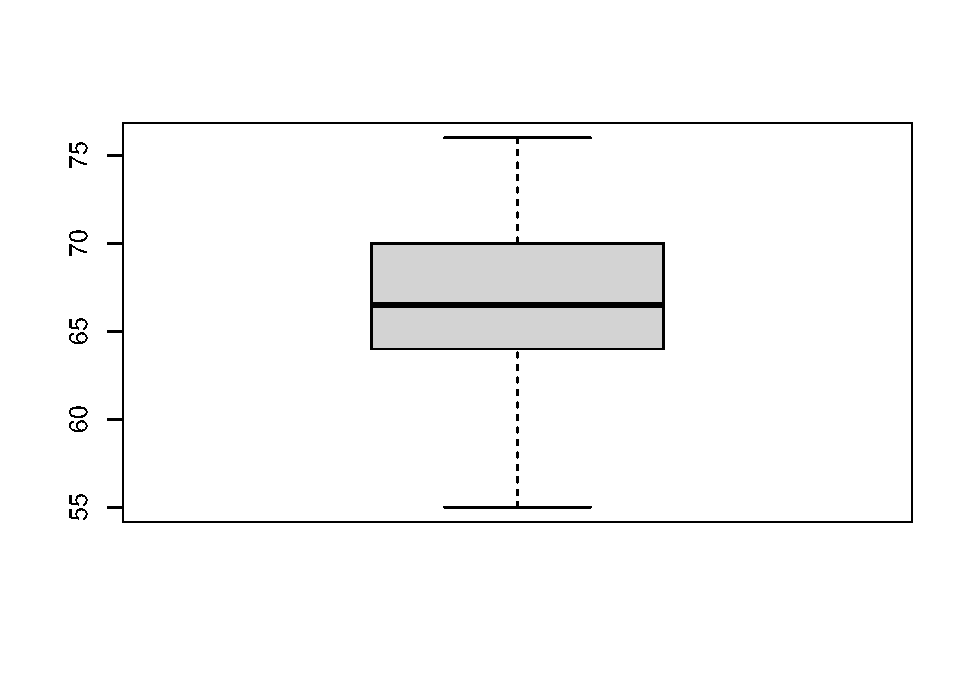
\includegraphics{_main_files/figure-latex/unnamed-chunk-77-1.pdf}

\hypertarget{continuous-data---histograms}{%
\subsection{Continuous Data - Histograms}\label{continuous-data---histograms}}

Continuous data, can also be broken into \textbf{bins} and plotted as a \textbf{histogram}. The \texttt{hist()} function will attempt to find the optimum number of bins for you, but you can specify a different number with the \texttt{breaks} argument.

\begin{Shaded}
\begin{Highlighting}[]
\FunctionTok{hist}\NormalTok{(data}\SpecialCharTok{$}\NormalTok{Height\_inches, }\AttributeTok{main =} \StringTok{"Histogram of Height"}\NormalTok{, }\AttributeTok{xlab =} \StringTok{"Height (in)"}\NormalTok{)}
\end{Highlighting}
\end{Shaded}

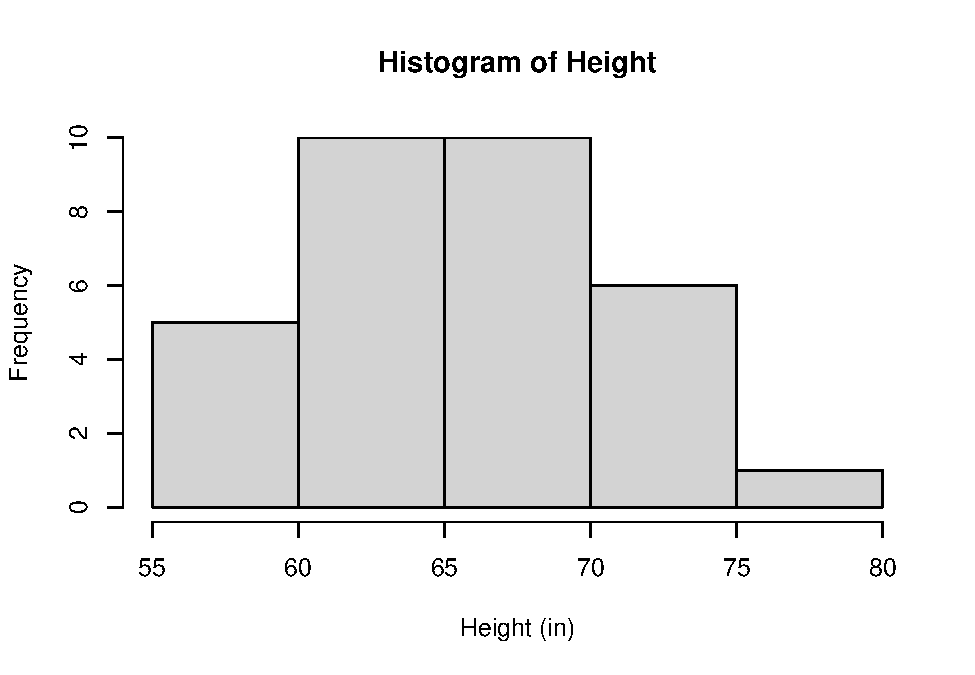
\includegraphics{_main_files/figure-latex/unnamed-chunk-78-1.pdf}

\hypertarget{categorical-data}{%
\subsection{Categorical Data}\label{categorical-data}}

Categorical data is already in discrete units. In general with categorical data, we want to count the \textbf{frequency} of unique values. There are many ways to do this, but one of the easiest is the \texttt{table()} function. Saving the results of the table to an object, \texttt{birth\_freq}, allows you to save and print the results at any time.

\begin{Shaded}
\begin{Highlighting}[]
\NormalTok{birth\_freq }\OtherTok{\textless{}{-}} \FunctionTok{table}\NormalTok{(data}\SpecialCharTok{$}\NormalTok{Birth\_Month)}

\NormalTok{birth\_freq}
\end{Highlighting}
\end{Shaded}

\begin{verbatim}
## 
##     April    August  December  February   January      July      June     March 
##         4         2         3         1         3         2         3         2 
##       May  November   October September 
##         4         4         2         2
\end{verbatim}

We can also visualize our tabulated results using a \textbf{barplot} as below.

\begin{Shaded}
\begin{Highlighting}[]
\FunctionTok{barplot}\NormalTok{(birth\_freq)}
\end{Highlighting}
\end{Shaded}

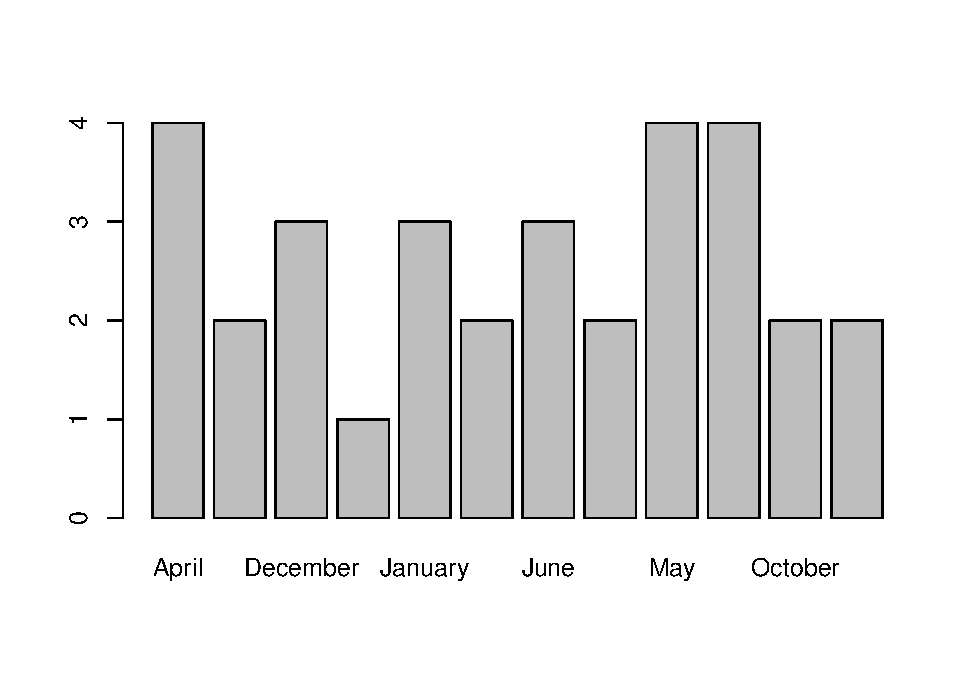
\includegraphics{_main_files/figure-latex/unnamed-chunk-80-1.pdf}

\hypertarget{glossary-2}{%
\section*{Glossary}\label{glossary-2}}
\addcontentsline{toc}{section}{Glossary}

\hypertarget{appendix-3b-additional-lessons-content-to-transfer-over-1}{%
\chapter*{Appendix 3b: Additional lessons / content to transfer over:}\label{appendix-3b-additional-lessons-content-to-transfer-over-1}}
\addcontentsline{toc}{chapter}{Appendix 3b: Additional lessons / content to transfer over:}

\hypertarget{comparing-data}{%
\section*{Comparing Data}\label{comparing-data}}
\addcontentsline{toc}{section}{Comparing Data}

\textbf{NEEDS A LOT OF WORK}

\hypertarget{data-distributions}{%
\section*{Data Distributions}\label{data-distributions}}
\addcontentsline{toc}{section}{Data Distributions}

\hypertarget{normal-distributions}{%
\subsection{Normal Distributions}\label{normal-distributions}}

First we'll generate a normal distribution with the \texttt{rnorm()} function. This takes 3 arguments: \texttt{n,\ mean,\ sd}, which you can see filled in below. While we could print out a list of all these values, it's not easy to \emph{understand} a list of numbers

\begin{Shaded}
\begin{Highlighting}[]
\NormalTok{normal\_dist }\OtherTok{\textless{}{-}} \FunctionTok{rnorm}\NormalTok{(}\AttributeTok{n =} \DecValTok{100}\NormalTok{, }\DocumentationTok{\#\# 100 samples}
                     \AttributeTok{mean =} \DecValTok{10}\NormalTok{, }\DocumentationTok{\#\# with a mean of 10}
                     \AttributeTok{sd =} \DecValTok{1} \DocumentationTok{\#\# and a standard deviation of 1}
\NormalTok{                     )}


\NormalTok{normal\_dist}
\end{Highlighting}
\end{Shaded}

\begin{verbatim}
##   [1] 11.537843  9.577027 11.444075 10.518058  9.752622  9.381794  9.283329
##   [8] 11.997276 10.383081 10.716883  9.871463 10.575796  9.803151  8.695750
##  [15]  9.346073  9.349846 10.108626 11.711685 10.674153 11.827317 11.779177
##  [22] 10.896859 12.545381 11.943484 10.964451  9.924096  9.439721 10.084466
##  [29] 10.287442  9.352893 10.636215  8.703583 10.935781 10.969983  8.645146
##  [36] 11.430844 11.295499 10.003588  8.291503  9.189448 11.316452 11.729021
##  [43] 11.006216 10.525947 10.863133  9.884728  8.801202 10.653382  9.648026
##  [50]  9.906731  7.851274  9.809432  9.968136  8.717939  9.882488 11.077242
##  [57] 10.287510  9.558057  9.327232 10.197740  7.510276 10.527043  9.925029
##  [64]  9.986464 10.820894  9.069265 10.166528  8.990858 11.031247 10.943931
##  [71]  8.493954  8.986688 10.595989  8.882771 10.572699 10.811687 10.045714
##  [78]  8.082443 10.578480 10.122678 10.514887  9.696846  9.871598  9.787594
##  [85] 10.141834  9.217790 10.534329 10.177832 10.412341 10.193418 10.332295
##  [92]  9.273755  9.637714  9.729498  9.926673 10.746631 10.008932  9.251834
##  [99] 12.293185  9.264603
\end{verbatim}

Another better way to look at data would be to \textbf{visualize} or \textbf{plot} it. One way to to that is with a \textbf{histogram}, which groups \textbf{continuous values} into \textbf{bins}, then plots the \textbf{frequency} for each bin.

In R, we use the \texttt{hist()} function to plot a histogram of data. We can (try to) control the number of bins with the \texttt{breaks} argument, but note that it doesn't always match up. The \texttt{hist()} function will adjust based on the distribution of the data.

\begin{Shaded}
\begin{Highlighting}[]
\FunctionTok{hist}\NormalTok{(normal\_dist,}\AttributeTok{breaks =} \DecValTok{5}\NormalTok{)}
\end{Highlighting}
\end{Shaded}

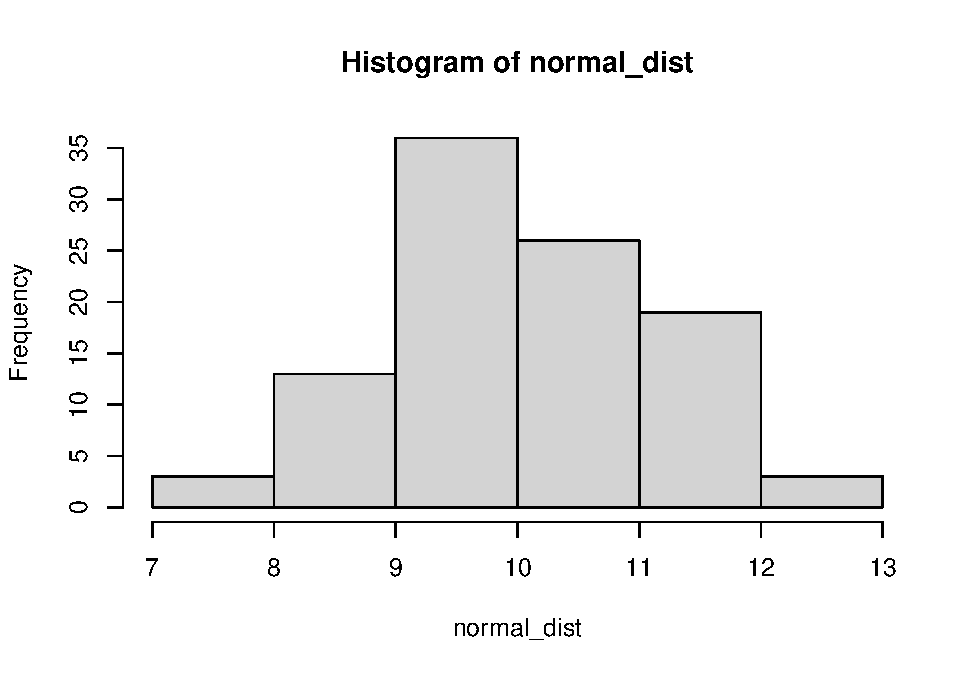
\includegraphics{_main_files/figure-latex/norm_dist_plot-1.pdf}

Another way to visualize this would be with a d

\hypertarget{what-is-normal}{%
\subsection{\texorpdfstring{What \emph{is} normal?}{What is normal?}}\label{what-is-normal}}

\hypertarget{quantitative-summaries}{%
\subsubsection{Quantitative summaries}\label{quantitative-summaries}}

5num summary
* Min, 25th percentile, median, 75th percentile, Max

\begin{Shaded}
\begin{Highlighting}[]
\NormalTok{tab\_normal\_dist }\OtherTok{\textless{}{-}} \FunctionTok{summary}\NormalTok{(normal\_dist)}
\end{Highlighting}
\end{Shaded}

We can print the table in R by calling its name.

\begin{Shaded}
\begin{Highlighting}[]
\NormalTok{tab\_normal\_dist}
\end{Highlighting}
\end{Shaded}

\begin{verbatim}
##    Min. 1st Qu.  Median    Mean 3rd Qu.    Max. 
##   7.510   9.425  10.097  10.120  10.724  12.545
\end{verbatim}

Mean, standard deviation

\hypertarget{meaningful-comparisons}{%
\subsubsection{Meaningful Comparisons}\label{meaningful-comparisons}}

How to compare apples to oranges? Standardize the units / standardize the data

\begin{Shaded}
\begin{Highlighting}[]
\NormalTok{data1 }\OtherTok{\textless{}{-}} \FunctionTok{rnorm}\NormalTok{(}\AttributeTok{n=}\DecValTok{1000}\NormalTok{, }
              \AttributeTok{mean =} \DecValTok{100}\NormalTok{,}
              \AttributeTok{sd =} \DecValTok{10}\NormalTok{)}

\NormalTok{data2 }\OtherTok{\textless{}{-}} \FunctionTok{rnorm}\NormalTok{(}\AttributeTok{n=}\DecValTok{1000}\NormalTok{,}
               \AttributeTok{mean =} \DecValTok{60}\NormalTok{, }
               \AttributeTok{sd =} \DecValTok{25}\NormalTok{)}
\end{Highlighting}
\end{Shaded}

Are these the same distribution?

Any issues??

\begin{Shaded}
\begin{Highlighting}[]
\FunctionTok{layout}\NormalTok{(}\FunctionTok{matrix}\NormalTok{(}\DecValTok{1}\SpecialCharTok{:}\DecValTok{2}\NormalTok{, }\AttributeTok{ncol =} \DecValTok{2}\NormalTok{))}
\FunctionTok{hist}\NormalTok{(data1)}
\FunctionTok{hist}\NormalTok{(data2)}
\end{Highlighting}
\end{Shaded}

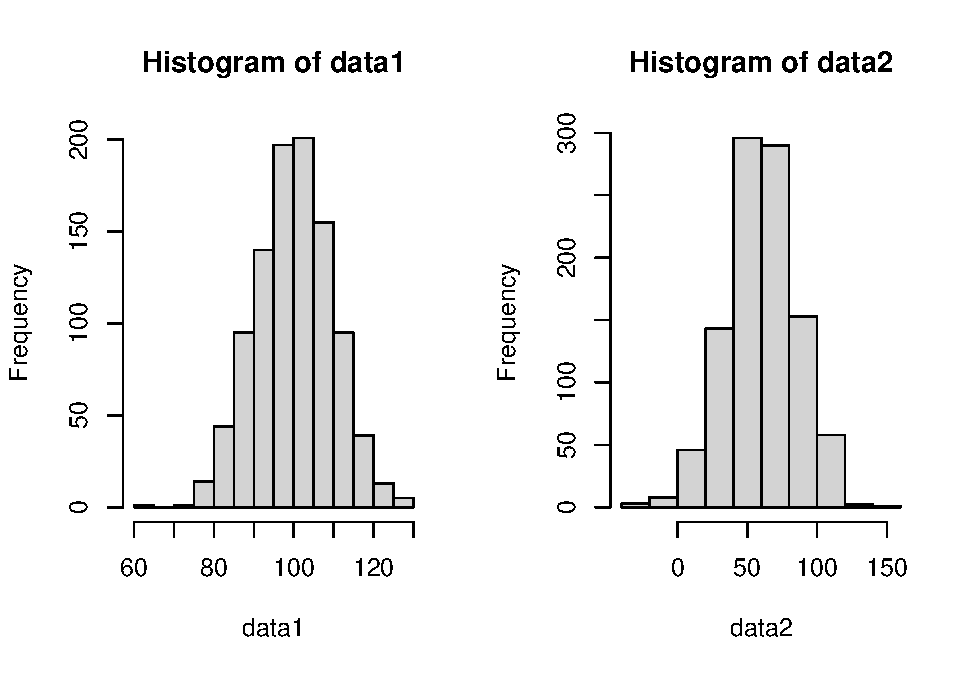
\includegraphics{_main_files/figure-latex/rnorm_hist_comp-1.pdf}

\begin{Shaded}
\begin{Highlighting}[]
\NormalTok{total\_range }\OtherTok{\textless{}{-}} \FunctionTok{range}\NormalTok{(data1, data2)}
\end{Highlighting}
\end{Shaded}

Are they the same?

\begin{Shaded}
\begin{Highlighting}[]
\FunctionTok{layout}\NormalTok{(}\FunctionTok{matrix}\NormalTok{(}\DecValTok{1}\SpecialCharTok{:}\DecValTok{2}\NormalTok{, }\AttributeTok{ncol =} \DecValTok{2}\NormalTok{))}
\FunctionTok{hist}\NormalTok{(data1, }\AttributeTok{xlim =}\NormalTok{ total\_range)}
\FunctionTok{hist}\NormalTok{(data2, }\AttributeTok{xlim =}\NormalTok{ total\_range)}
\end{Highlighting}
\end{Shaded}

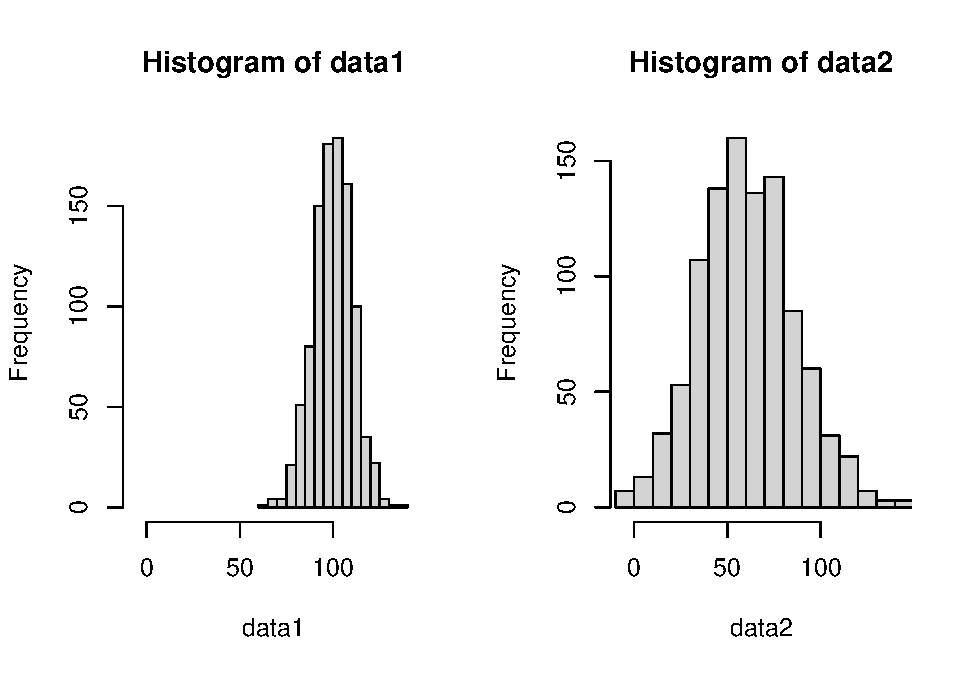
\includegraphics{_main_files/figure-latex/rnorm_hist_comp_true-1.pdf}

Numerically / tabularly

Often times its important to tables of \textbf{summary statistics}

\begin{Shaded}
\begin{Highlighting}[]
\NormalTok{norm\_comp\_tab }\OtherTok{\textless{}{-}} \FunctionTok{rbind}\NormalTok{(}\FunctionTok{summary}\NormalTok{(data1),}
                       \FunctionTok{summary}\NormalTok{(data2))}

\NormalTok{norm\_comp\_tab}
\end{Highlighting}
\end{Shaded}

\begin{verbatim}
##           Min.  1st Qu.   Median     Mean   3rd Qu.     Max.
## [1,]  67.50282 92.94738 99.85491 99.83723 106.34225 127.6897
## [2,] -11.47190 44.40308 60.78438 61.91661  79.79141 142.9623
\end{verbatim}

Making the table a little nicer. Also an example of \textbf{conditional programming}.

\begin{Shaded}
\begin{Highlighting}[]
\FunctionTok{rownames}\NormalTok{(norm\_comp\_tab) }\DocumentationTok{\#\# they\textquotesingle{}re null}
\end{Highlighting}
\end{Shaded}

\begin{verbatim}
## NULL
\end{verbatim}

\begin{Shaded}
\begin{Highlighting}[]
\ControlFlowTok{if}\NormalTok{(}\FunctionTok{is.null}\NormalTok{(}\FunctionTok{rownames}\NormalTok{(norm\_comp\_tab)))\{}
  \FunctionTok{rownames}\NormalTok{(norm\_comp\_tab) }\OtherTok{\textless{}{-}} \FunctionTok{c}\NormalTok{(}\StringTok{"data1"}\NormalTok{, }\StringTok{"data2"}\NormalTok{)}
\NormalTok{\}}
\end{Highlighting}
\end{Shaded}

When working with \textbf{Rmarkdown} we can take advantage of \texttt{knitr} and \texttt{pandoc} to nice looking tables even easier.

\begin{Shaded}
\begin{Highlighting}[]
\NormalTok{knitr}\SpecialCharTok{::}\FunctionTok{kable}\NormalTok{(norm\_comp\_tab)}
\end{Highlighting}
\end{Shaded}

\begin{tabular}{l|r|r|r|r|r|r}
\hline
  & Min. & 1st Qu. & Median & Mean & 3rd Qu. & Max.\\
\hline
data1 & 67.50282 & 92.94738 & 99.85491 & 99.83723 & 106.34225 & 127.6897\\
\hline
data2 & -11.47190 & 44.40308 & 60.78438 & 61.91661 & 79.79141 & 142.9623\\
\hline
\end{tabular}

\textbf{How} transform the data

Simple transformation (multiply all values by 100)
* to convert units
* other examples?

Complex transformations
* log-transformation (\emph{DEE: not a fan})
* z-scores (\emph{DEE: a better option})

\textbf{Why} transform the data?
* Real world applications?
* Is it always appropriate to transform data?

\hypertarget{skews}{%
\subsection{Skews}\label{skews}}

What to do if the data are \textbf{not} normal?

\hypertarget{statisitcal-testing-of-simple-data-sets}{%
\section*{Statisitcal testing of simple data sets}\label{statisitcal-testing-of-simple-data-sets}}
\addcontentsline{toc}{section}{Statisitcal testing of simple data sets}

\hypertarget{t-tests-anova-chi2}{%
\subsection{t-tests, ANOVA, chi2}\label{t-tests-anova-chi2}}

\hypertarget{relationships-between-variables-in-simple-data-sets}{%
\section*{Relationships between variables in simple data sets}\label{relationships-between-variables-in-simple-data-sets}}
\addcontentsline{toc}{section}{Relationships between variables in simple data sets}

\hypertarget{correlation-linear-regression}{%
\subsection{Correlation, Linear Regression}\label{correlation-linear-regression}}

\hypertarget{simple-lm}{%
\subsubsection{Simple LM}\label{simple-lm}}

\hypertarget{complex-lm}{%
\subsubsection{Complex LM}\label{complex-lm}}

\hypertarget{genearlized-linear-model}{%
\subsection{Genearlized Linear Model}\label{genearlized-linear-model}}

For now, I have 3 main chapters for each of the main sections:
* Basics of data science / R
* Applications/critiques using IPUMS data
* Student-driven projects

Each of these \textbf{Chapters} contains multiple sections. We'll likely want to break these sections out into their own \texttt{.Rmd} files as they get fleshed out. For now, I'll try to keep the abundance of files limited.

\textbf{NOTE:} As these actually get filled out, we will probably want to insert different \texttt{part}s to the book (EG, the content of Unit 1 is covered in \texttt{Part\ I}).
* Declare parts with \texttt{\#\ (PART)\ Part\ I\ \{-\}} immediately before the first chapter \texttt{\#} it contains.

\textbf{Topics to include:}
* What is data?
* Everything can be data
* How do we interpret data
* Tables
* Plots
* Univariate distributions
* What can they tell us
* Multi-modality in distributions
* Categorical vs continuous data
* Don't need to get ahead of this yet
* Add in a grouping category - multi state/multi-national dataset
* Ttest / anova

\textbf{Type of Data:}
Age distributions
Specifically generate a dataset with old/young folks over-represented to highlight a bimodal distribution

Start with single state/country
Add a second state/country to demo ttest
Add more to demo anova

Alternatively, income by education level - may be more interesting/relevant to college students (or depressing)

\hypertarget{intro-to-rrstudio}{%
\section*{Intro to R/RStudio}\label{intro-to-rrstudio}}
\addcontentsline{toc}{section}{Intro to R/RStudio}

\hypertarget{reading-data-distributions}{%
\section*{Reading Data / Distributions}\label{reading-data-distributions}}
\addcontentsline{toc}{section}{Reading Data / Distributions}

\hypertarget{what-is-a-normal-distribution}{%
\subsection{\texorpdfstring{What \emph{is} a \textbf{normal distribution}}{What is a normal distribution}}\label{what-is-a-normal-distribution}}

\hypertarget{how-normal-is-it}{%
\subsubsection{How normal is it?}\label{how-normal-is-it}}

show increasingly unclear examples of normal vs not

introduce tests of normality

\hypertarget{measuring-normality---single-sample}{%
\subsubsection{Measuring normality - single sample}\label{measuring-normality---single-sample}}

reinforce {[}concept of statistical{]} \textbf{normality}

is a value from a sample? - one way ttest
something about tails

\hypertarget{comparing-normality---two-saples}{%
\subsubsection{comparing normality - two saples}\label{comparing-normality---two-saples}}

standard / two-way t test

\hypertarget{comparing-more-than-two---anova}{%
\subsubsection{comparing more than two - ANOVA}\label{comparing-more-than-two---anova}}

\hypertarget{glossary-3}{%
\section*{Glossary}\label{glossary-3}}
\addcontentsline{toc}{section}{Glossary}

Data
Quantitative
Qualitative
Discrete
Continuous
Nominal
Ordinal

\hypertarget{dev-appendix-styling-with-rmd}{%
\chapter*{dev-Appendix : Styling with RMD}\label{dev-appendix-styling-with-rmd}}
\addcontentsline{toc}{chapter}{dev-Appendix : Styling with RMD}

For now, this chapter is a bit of a placeholder. I'm not sure what/how
the \texttt{references.Rmd} file actually fits in to the code/construction (it
looks automatic) so I want to keep that in place and need a section to
note that.

I also want a more centralized reference point to put any example code I
find helpful while working in R/bookdown. This section could get really
unruly really fast, but oh well.

\hypertarget{navigating-the-bookdown}{%
\section*{Navigating the bookdown}\label{navigating-the-bookdown}}
\addcontentsline{toc}{section}{Navigating the bookdown}

All chapter files need a 2 digit prefix (except \texttt{index.Rmd}) which
dictates the chapter order. Note, this is not automatic and a little
tedious to re-do.

\begin{itemize}
\item
  \texttt{index.Rmd} is a required file and treated as file
  \texttt{00}.
\item
  Chapters \emph{should} be numbered for ease of sorting but custom
  orders are possible by specifying filenames somewhere \texttt{in\ a\ certain\ file...but\ i\textquotesingle{}m\ not\ sure\ where}.
\end{itemize}

Remember each Rmd file contains one and only one chapter, and a chapter
is defined by the first-level heading \texttt{\#}.
* Unlike usual Rmd files, chapters DO not contain a YAML header
* Note that \texttt{index.Rmd} has its own YMAL for the title page and some bookwide parameters.

\hypertarget{include-images}{%
\section*{Include Images}\label{include-images}}
\addcontentsline{toc}{section}{Include Images}

\hypertarget{figures-in-a-folder}{%
\subsection{Figures in a folder}\label{figures-in-a-folder}}

Embed figures from a folder.

For this, it's usually best to use a code-chunk and \texttt{knitr}. There are a
number of graphical paramerters you can set (or ignore) \texttt{out.width} will
scale your image accordingly - irrespective of unit/display \texttt{fig.align}
should be ``left'', ``right'', or ``center'' \texttt{fig.cap} allows you to provide
``mouse over'' captions for the image. \texttt{echo=FALSE} is important if you
ONLY want the image (IE the result of the code). If you want the code
itself to show, (IE, or echo) set \texttt{echo=TRUE}.

\begin{figure}

{\centering 
\includegraphics[width=0.5\linewidth]{imgs/ipums_i_logo} 

}

\caption{the ipums logo}\label{fig:unnamed-chunk-88}
\end{figure}

\hypertarget{fancy-renders}{%
\subsection{Fancy renders}\label{fancy-renders}}

Embed html renders (EG, fancy tables (IPUMS\_var\_desc), or any shiny app)
with \texttt{webshot} R package and \texttt{phantomJS}.

\begin{Shaded}
\begin{Highlighting}[]
\FunctionTok{install.packages}\NormalTok{(}\StringTok{"webshot"}\NormalTok{)}
\NormalTok{webshot}\SpecialCharTok{::}\FunctionTok{install\_phantomjs}\NormalTok{()}
\end{Highlighting}
\end{Shaded}

\hypertarget{tips}{%
\section*{Tips}\label{tips}}
\addcontentsline{toc}{section}{Tips}

\begin{itemize}
\tightlist
\item
  Each section (chapters) gets \textbf{AUTOMATIC NUMBERING}

  \begin{itemize}
  \tightlist
  \item
    Use \texttt{\{-\}} or \texttt{\{.unnumbered\}} to keep a section out of the auto-list. These will still be listed in the TOC
  \item
    To hide the heading from the TOC you can also use \{.unlisted\}
  \end{itemize}
\end{itemize}

\hypertarget{basic-fonts}{%
\section*{Basic Fonts}\label{basic-fonts}}
\addcontentsline{toc}{section}{Basic Fonts}

In a list:

\begin{itemize}
\item
  \emph{italics}
\item
  \textbf{bold}
\item
  \texttt{code}
\item
  \(equations\)
\end{itemize}

In \emph{a sentence} \textbf{with differently} \texttt{formated\ fonts} and maths \$ a + b
= c? \$.

\hypertarget{more-on-math}{%
\subsection{More on Math}\label{more-on-math}}

Randal Pruim features an extensive list of common math expression on
their \href{https://rpruim.github.io/s341/S19/from-class/MathinRmd.html}{github
page}. Here
are some quick notes:

In-line equations can be written within \texttt{\$} and will be displayed right
there: \(a^2 + b^2 = c^2\). In contrast, you can also add equation-chunks
by using \texttt{\$\$}

This can be coded in-line, \[\sum_{n=1}^{10} n^2\], but will result in a
page break.

\(p\) is unknown but expected to be around 1/3. Standard error will be
approximated

\[
SE = \sqrt(\frac{p(1-p)}{n}) \approx \sqrt{\frac{1/3 (1 - 1/3)} {300}} = 0.027
\]

\hypertarget{linking-and-crossrefs}{%
\section*{Linking and Crossrefs}\label{linking-and-crossrefs}}
\addcontentsline{toc}{section}{Linking and Crossrefs}

There are a few different options here:

\begin{itemize}
\item
  Footnotes
\item
  Hyperlinks
\item
  autocite?
\end{itemize}

\hypertarget{footntes}{%
\subsection{Footntes}\label{footntes}}

You can also use math in footnotes like this\footnote{where we mention \(p = \frac{a}{b}\)}. Footnotes
are helpful because they either open to a new page, where you can
re-link to where you left off. Or they display as a literal footnote,
depending on your file format.

We will approximate standard error to 0.027\footnote{\(p\) is unknown but expected to be around 1/3. Standard
  error will be approximated

  \[
  SE = \sqrt(\frac{p(1-p)}{n}) \approx \sqrt{\frac{1/3 (1 - 1/3)} {300}} = 0.027
  \]}

Anything that maintains the indent following the html tag (square
brackets) will be included in the footnote and \textbf{excluded} from the
actual rendered text. This could be helpful to easily provide more
information without breaking the narrative; however, it has the drawback
that footnotes are dispersed throughout the document.

\textbf{NOTE:} Footnote labels can be any character string, but for our own
sakes, it makes sense to follow a standard, descriptive, format.

To compile this example to PDF, you need XeLaTeX. You are recommended to
install TinyTeX (which includes XeLaTeX): \url{https://yihui.name/tinytex/}.

\hypertarget{hyperlinks}{%
\subsection{Hyperlinks}\label{hyperlinks}}

In short, if you \textbf{label} it, you can link to it. So it's good practice to
\textbf{LABEL EVERYTHING DESCRIPTIVELY} in case you it later. There are a couple of differnt styles of labeling depending on what you want to link to. You already saw above how to link to a website (URL).

\begin{itemize}
\tightlist
\item
  code chunks that produce figures can be referenced via \texttt{@\textbackslash{}ref(fig:{[}LABEL{]})}
\end{itemize}

\hypertarget{link-to-chapters}{%
\subsubsection{Link to chapters}\label{link-to-chapters}}

You can label chapter, section, or any level of header (\texttt{\#\#}) using by including the label in curly brackets after the section.
* e.g., we can reference @ref(unit1\_ch1) using the following:
+ \texttt{\textbackslash{}@ref(unit1\_ch1)}

\textbf{NOTE:} If you do not manually label sections, they will get automatic labels anyway, which are hard to reference, so best to just declare them.

\hypertarget{link-to-figures-tables-or-code-chunks}{%
\subsubsection{Link to figures, tables, or code chunks}\label{link-to-figures-tables-or-code-chunks}}

You can link to figures or tables created by R code, or the R code itself, as long as they are labeled.
\textbf{Be careful!!} if labels are not descriptive and informative, it might be hard to find them later.
* We should decide on some conventions for this!*

Whatever the output (figure, table, etc), the label follows the r at the very first line of the code chunk:
* \texttt{\{r\ an\_example\}\textasciigrave{}\ \ \ *}\{r an\_example, fig.cap = ``Example that include additional code chunk parameters''\}`

To include the link in text, use the \texttt{\textbackslash{}@ref()}.

To link to the code itself, we simply call the label (just like linking to a section header).
* \texttt{\textbackslash{}@ref(basic\_code)} Link to some basic code @ref(basic\_code)

If the output is a figure, you will also need to preface the label with \texttt{fig:}
* \texttt{\textbackslash{}@ref(fig:height\_boxplot)}. Is the code that produces this link to a figure @ref(fig:height\_boxplot)

In order to reference a nicely formatted table, made with \texttt{knitr::kable()}, use the following:
* \texttt{\textbackslash{}@ref(tab:height\_table)}. In order to reference \emph{this table} @ref(tab:height\_table)

\hypertarget{link-to-websites}{%
\subsubsection{Link to websites}\label{link-to-websites}}

linking to external websites is easy, just include the \href{https://ehrlichd.github.io/ipumsEDbook}{text-to-be-hyperlinked}

This is actuall the exact same as linking to a local .jpg or similar.

\hypertarget{citations}{%
\subsection{Citations}\label{citations}}

There do appera to be tools for citations, but I'm not super familiar with them so this section will grow as I learn more.

\hypertarget{citing-r-packages}{%
\subsubsection{Citing R packages}\label{citing-r-packages}}

You can easily gather a list of all R packages used in a project using \texttt{knitr::write\_bib()}.
By using square brackets and the \texttt{@} sign, along with the package name? or maybe the github repo? I'm not entirely sure, see below

Quick example from demo/index (may not work without write\_bib() though):
we are using the \textbf{bookdown} package \citep{R-bookdown} in this sample book,
which was built on top of R Markdown and \textbf{knitr} \citep{xie2015}.

\begin{itemize}
\tightlist
\item
  This infor should be written to the References files, though i'm not sure if it will work
\end{itemize}

\hypertarget{glossary-4}{%
\chapter{Glossary}\label{glossary-4}}

\hypertarget{unit-1}{%
\section{Unit 1}\label{unit-1}}

\hypertarget{chapter-1}{%
\subsection{Chapter 1}\label{chapter-1}}

\textbf{Random Sampling:}
\textbf{Stratified Random Sampling:}
\textbf{Statistical bias}

\hypertarget{aoendix-1}{%
\section{Aoendix 1}\label{aoendix-1}}

\hypertarget{intro-to-r}{%
\subsection{Intro to R}\label{intro-to-r}}

\hypertarget{advanced-methods}{%
\chapter*{Advanced Methods}\label{advanced-methods}}
\addcontentsline{toc}{chapter}{Advanced Methods}

  \bibliography{book.bib,packages.bib}

\end{document}
